\documentclass[11pt]{beamer}
\usepackage{graphicx}
\usepackage[export]{adjustbox}  % max width/height in includegraphics
\usepackage{xcolor}
\usepackage{ifthen}
\usepackage{fontspec}
\usepackage{textcomp}
%\usepackage[T5,T1]{fontenc}
\usepackage{caption}

\usepackage{verse}
\newcommand{\attrib}[1]{%
\nopagebreak{\raggedleft\footnotesize #1\par}}
\renewcommand{\poemtitlefont}{\normalfont\large\itshape\centering}

\usetheme[hideothersubsections]{Goettingen}
\usecolortheme{seahorse}
%%% \usetheme{Montpellier}
%%% \usecolortheme{dolphin}
\setbeamercovered{invisible}
\setbeamertemplate{navigation symbols}{\insertslidenavigationsymbol}
\setbeamertemplate{page number in head/foot}{}
\setbeamertemplate{blocks}[rounded][shadow=false]
% \setbeamerfont{section in sidebar}{size=\fontsize{4}{3}\selectfont}
% \setbeamerfont{subsection in sidebar}{size=\fontsize{4}{3}\selectfont}
% \setbeamerfont{subsubsection in sidebar}{size=\fontsize{4}{2}\selectfont}

\usepackage{microtype}
% \DisableLigatures[f]{encoding = *, family = *}

% \usefonttheme{professionalfonts} % using non standard fonts for beamer
\usepackage{tgheros}
\usefonttheme{serif}
\usepackage{XCharter}

\AtBeginSection[]{
  \begin{frame}
    \vfill
    \centering
    \begin{beamercolorbox}[sep=8pt,center,shadow=true,rounded=true]{title}
    \usebeamerfont{title}\insertsectionhead\par%
    \ifthenelse{\equal{\thisSectionName}{Bonus}}{}{
        \usebeamerfont{subtitle}\thisSectionName\par%
    }
    \end{beamercolorbox}
    \begin{center}
    \ifthenelse{\equal{\thisSectionName}{Colleges and Universities}}{
        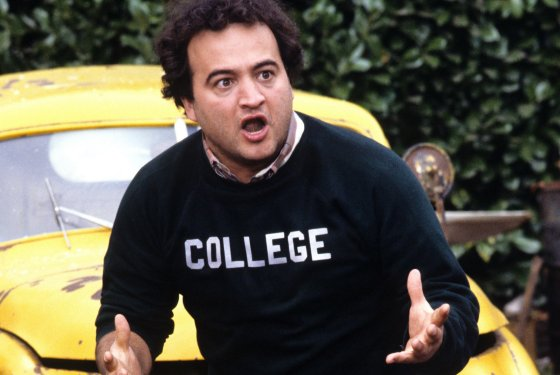
\includegraphics[max height = 0.3\textheight]{Images/belushicollege.jpg}
    }{}

    Please mute yourselves!
    \end{center}

    \ifthenelse{\equal{\thisSectionName}{Bonus}}
    {
        Get ready for some \emph{devilishly} hard questions!

        \vspace*{1em}
        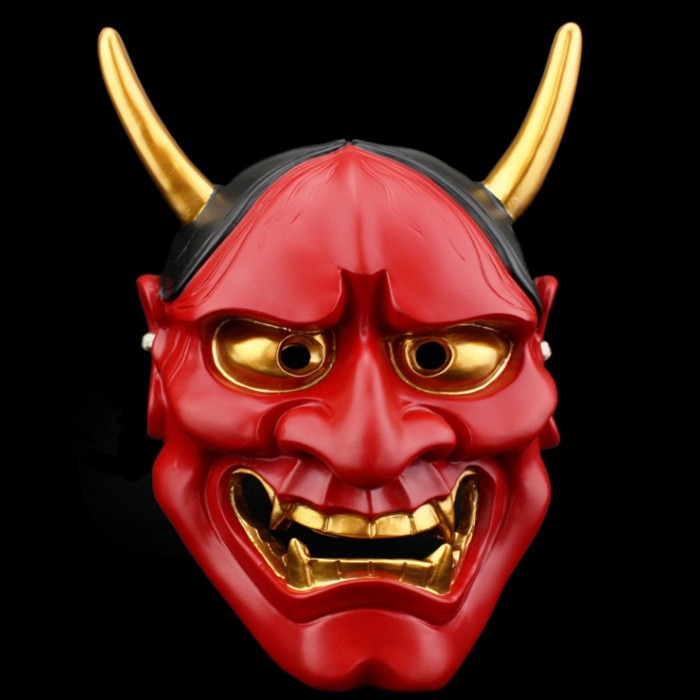
\includegraphics[max width=0.5\textwidth,
           max height=0.4\textheight]{Images/devil.jpg}
    }{}

    \vfill
  \end{frame}
}

\AtBeginSubsection[]{
  \begin{frame}
    \vfill
    \centering
    \begin{beamercolorbox}[sep=8pt,center,shadow=true,rounded=true]{title}
    \usebeamerfont{title}\insertsectionhead\par%
    \usebeamerfont{subtitle}\insertsubsectionhead\par%
    \end{beamercolorbox}
    \ifthenelse{\equal{\subsecname}{Answers}} {
        \begin{center}
        Unmute yourselves!
        \end{center}
    }
    \vfill
  \end{frame}
}
\begin{document}

\title{Welcome to Curfew Trivia I / Quarantine Trivia X!}
\date{}

\begin{frame}
\titlepage{}
\begin{center}

\includegraphics[max width=0.9\textwidth,
    max height=0.4\textheight]{Images/triviatitleframelogo.png}
\end{center}
\end{frame}

\begingroup{}
\begin{frame}{}
Since this is Game 10, we'd like to look back over a few of the more ``interesting''
questions from the last nine games.
\end{frame}
\begin{frame}{}
First, we failed to distinguish between beignets and zeppole.

\begin{figure}
\captionsetup{labelformat=empty}
\centering
\begin{minipage}{.5\textwidth}
  \centering
  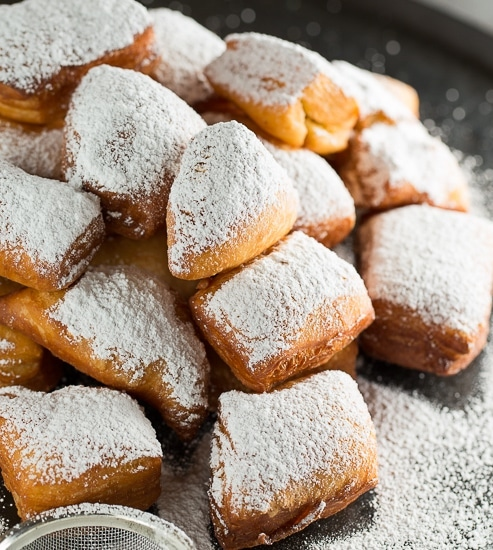
\includegraphics[height=.4\textheight]{Images/beignets.jpg}
  \captionof{figure}{Beignets (maybe?)}
\end{minipage}%
\begin{minipage}{.5\textwidth}
  \centering
  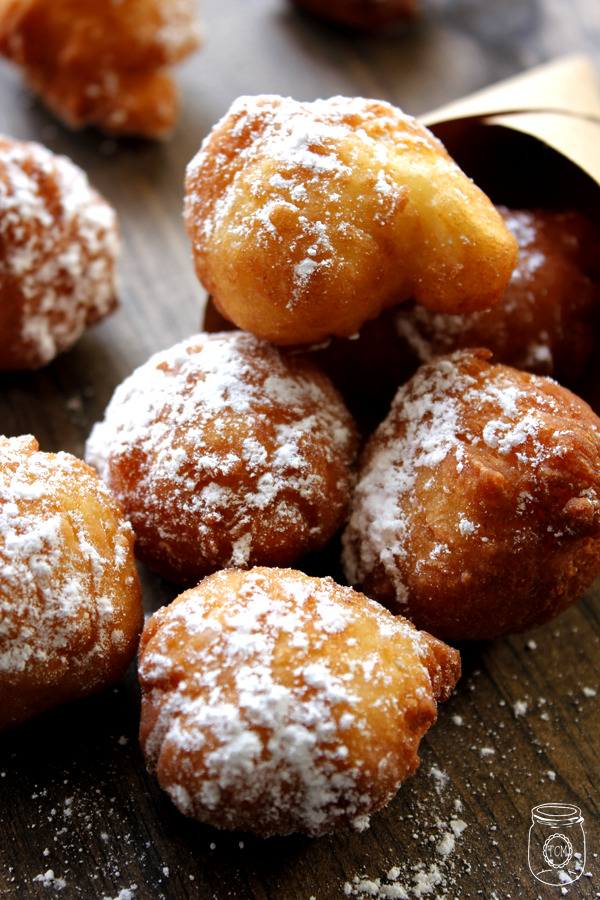
\includegraphics[height=.4\textheight]{Images/zeppole.jpg}
  \captionof{figure}{Zeppole (could be?)}
\end{minipage}
\end{figure}
\end{frame}
\begin{frame}{}
\medskip{}
Then, we introduced you to the poetry of Emily Dickson:
\pause{}
\vspace*{0.5in}
\settowidth{\versewidth}{Because I could not stop for meth}
\begin{verse}[\versewidth]
Because I could not stop for meth --- \\
I had it delivered --- \ldots{}
\end{verse}
\attrib{Emily Dickson}
\end{frame}
\begin{frame}{}
\medskip{}
We took a political stance on the meaning of the word ``Ireland''.
\begin{center}

\includegraphics[max width=0.9\textwidth,max height=0.5\textheight
]{Images/ireland.png}
\end{center}
\end{frame}
\begin{frame}{}
\medskip{}
And finally, we displayed cuneiform backwards, which we know confused everyone.
\end{frame}
\begin{frame}
So for all of these mistakes, we wish to say \ldots{}
\pause{}
\begin{center}
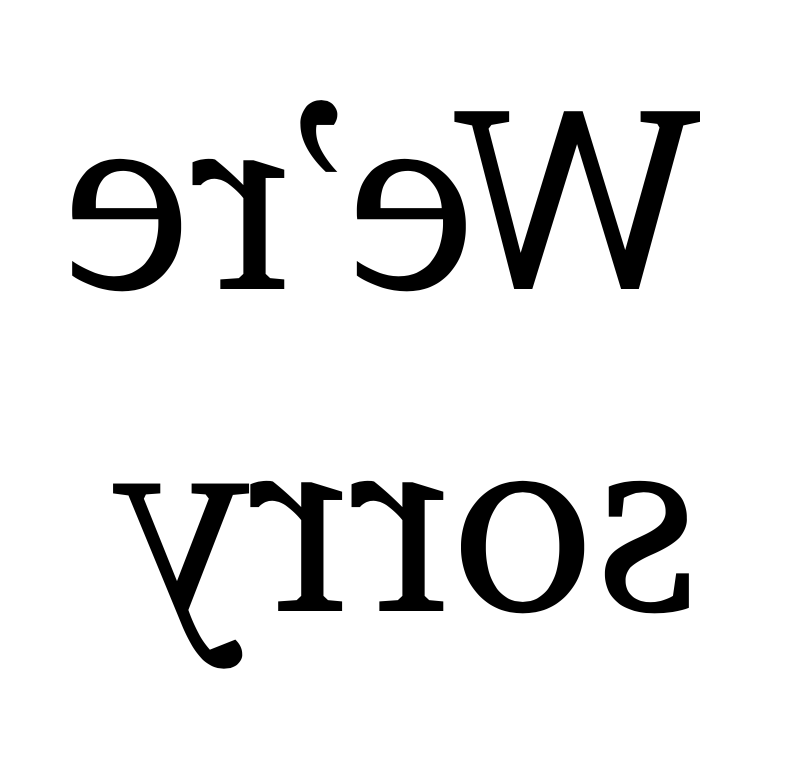
\includegraphics[max width=0.9\textwidth,max height=0.5\textheight
    ]{Images/cuneiform.png}
\end{center}

\end{frame}
\endgroup{}

\begin{frame}{}
\medskip{}
So now let's see what's in store for this week \ldots{}
\end{frame}


\begingroup{}
\begin{frame}[t]{Categories}
This week, you'll be answering questions in the following categories:
\begin{enumerate}
\item Quotations
\item East Asia
\item Musical Instruments
\item Outer Space
\item Saturday Night Live
\item Special Words from Various Fields
\item Streets, Highways and Boulevards
\item The Biggest and the Most
\item The Wild West
\item Who Originated the Role?
\end{enumerate}
\end{frame}
\endgroup{}

\begingroup{}
\begin{frame}
\vfill{}
\begin{beamercolorbox}[sep=8pt,center,shadow=true,rounded=true]{title}
\usebeamerfont{title}Good luck everyone! And have fun!
\end{beamercolorbox}
\vfill{}
\end{frame}
\endgroup{}
\def\thisSectionName{Quotations}
\section{Round 1}
\subsection*{Q1}
\begin{frame}[t]{Round 1 --- Quotations --- \mbox{Question 1}}
\vspace{-0.5em}
\begin{block}{Question}
``Veni vidi vici.''
\end{block}
\end{frame}
\subsection*{Q2}
\begin{frame}[t]{Round 1 --- Quotations --- \mbox{Question 2}}
\vspace{-0.5em}
\begin{block}{Question}
``To be prepared for war is one of the most effectual means of preserving peace.''
\end{block}
\end{frame}
\subsection*{Q3}
\begin{frame}[t]{Round 1 --- Quotations --- \mbox{Question 3}}
\vspace{-0.5em}
\begin{block}{Question}
``When you come to a fork in the road, take it!''
\end{block}
\end{frame}
\subsection*{Q4}
\begin{frame}[t]{Round 1 --- Quotations --- \mbox{Question 4}}
\vspace{-0.5em}
\begin{block}{Question}
``Be the change that you wish to see in the world.''
\end{block}
\end{frame}
\subsection*{Q5}
\begin{frame}[t]{Round 1 --- Quotations --- \mbox{Question 5}}
\vspace{-0.5em}
\begin{block}{Question}
``The reports of my death are greatly exaggerated.''
\end{block}
\end{frame}
\subsection*{Q6}
\begin{frame}[t]{Round 1 --- Quotations --- \mbox{Question 6}}
\vspace{-0.5em}
\begin{block}{Question}
``I am the straw that stirs the drink'' has been attributed to which athlete (who has denied saying it)?
\end{block}
\end{frame}
\subsection*{Q7}
\begin{frame}[t]{Round 1 --- Quotations --- \mbox{Question 7}}
\vspace{-0.5em}
\begin{block}{Question}
``Always forgive your enemies; nothing annoys them so much.''
\end{block}
\end{frame}
\subsection*{Q8}
\begin{frame}[t]{Round 1 --- Quotations --- \mbox{Question 8}}
\vspace{-0.5em}
\begin{block}{Question}
``When you are courting a nice girl an hour seems like a second. When you sit on a red-hot cinder a second seems like an hour.''
\end{block}
\end{frame}
\subsection*{Q9}
\begin{frame}[t]{Round 1 --- Quotations --- \mbox{Question 9}}
\vspace{-0.5em}
\begin{block}{Question}
``If I were two-faced, would I be wearing this one?''
\end{block}
\end{frame}
\subsection*{Q10}
\begin{frame}[t]{Round 1 --- Quotations --- \mbox{Question 10}}
\vspace{-0.5em}
\begin{block}{Question}
Which Shakespeare character says, ``If you prick us, do we not bleed? If you tickle us, do we not laugh?''
\end{block}
\end{frame}
\subsection{Answers}
\begin{frame}[t]{Round 1 --- Quotations --- \mbox{Answer 1}}
\vspace{-0.5em}
\begin{block}{Question}
``Veni vidi vici.''
\end{block}

\visible<2->{
    \begin{columns}[T,totalwidth=\linewidth]
    \begin{column}{0.32\linewidth}
    \begin{block}{Answer}
    Julius Caesar
    \end{block}
    \end{column}
    \begin{column}{0.65\linewidth}
    \begin{center}
    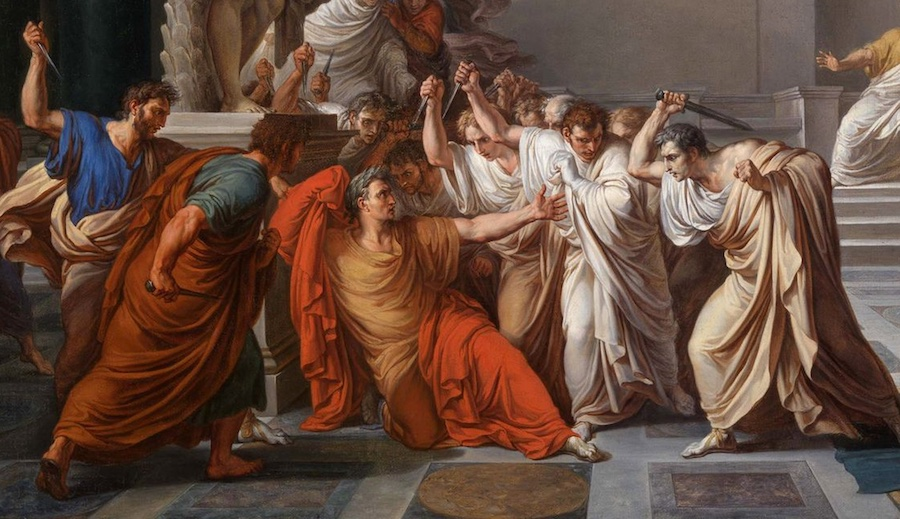
\includegraphics[max width=0.95\textwidth,
        max height=0.58000\textheight]{{Images/caesar}.jpg}
    \end{center}
    \end{column}
    \end{columns}
}
\end{frame}
\begin{frame}[t]{Round 1 --- Quotations --- \mbox{Answer 2}}
\vspace{-0.5em}
\begin{block}{Question}
``To be prepared for war is one of the most effectual means of preserving peace.''
\end{block}

\visible<2->{
    \begin{columns}[T,totalwidth=\linewidth]
    \begin{column}{0.32\linewidth}
    \begin{block}{Answer}
    George Washington
    \end{block}
    \end{column}
    \begin{column}{0.65\linewidth}
    \begin{center}
    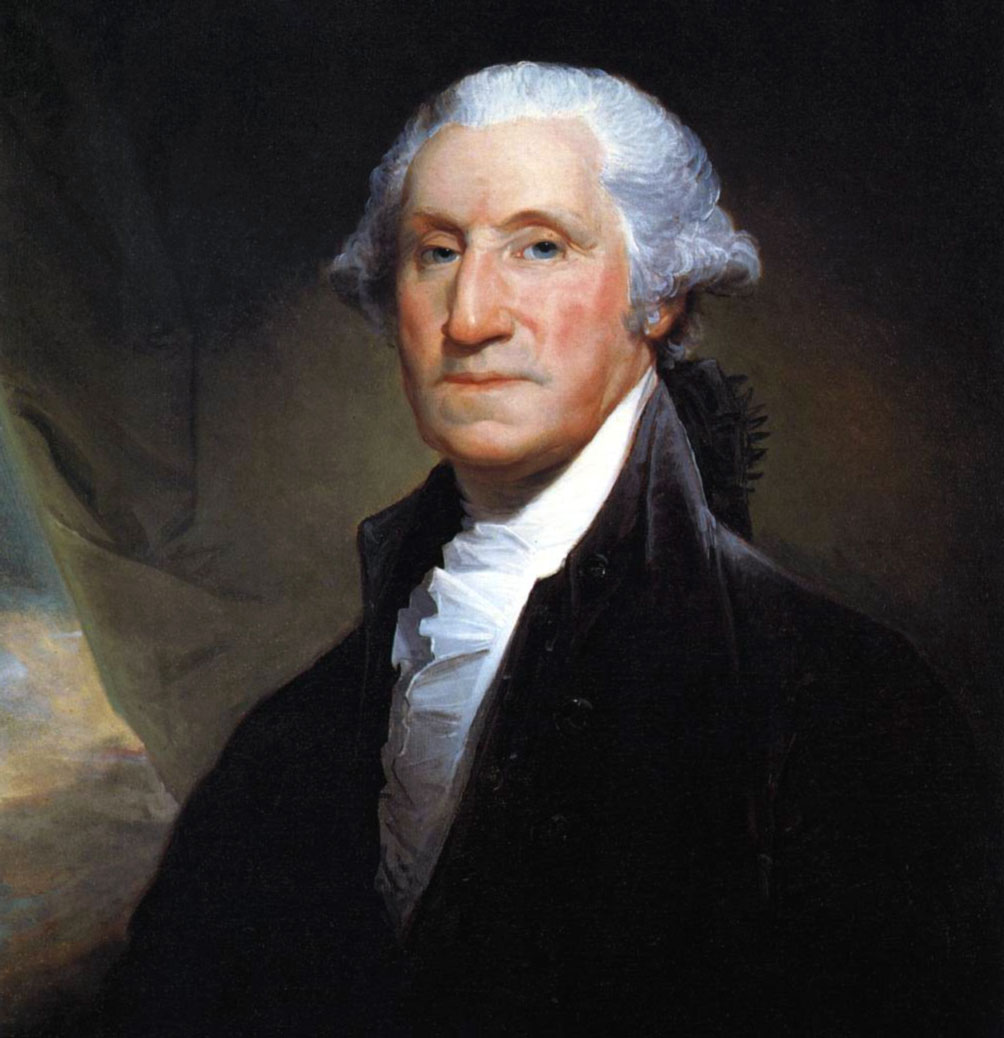
\includegraphics[max width=0.95\textwidth,
        max height=0.54000\textheight]{{Images/washington}.jpg}
    \end{center}
    \end{column}
    \end{columns}
}
\end{frame}
\begin{frame}[t]{Round 1 --- Quotations --- \mbox{Answer 3}}
\vspace{-0.5em}
\begin{block}{Question}
``When you come to a fork in the road, take it!''
\end{block}

\visible<2->{
    \begin{columns}[T,totalwidth=\linewidth]
    \begin{column}{0.32\linewidth}
    \begin{block}{Answer}
    Yogi Berra
    \end{block}
    \end{column}
    \begin{column}{0.65\linewidth}
    \begin{center}
    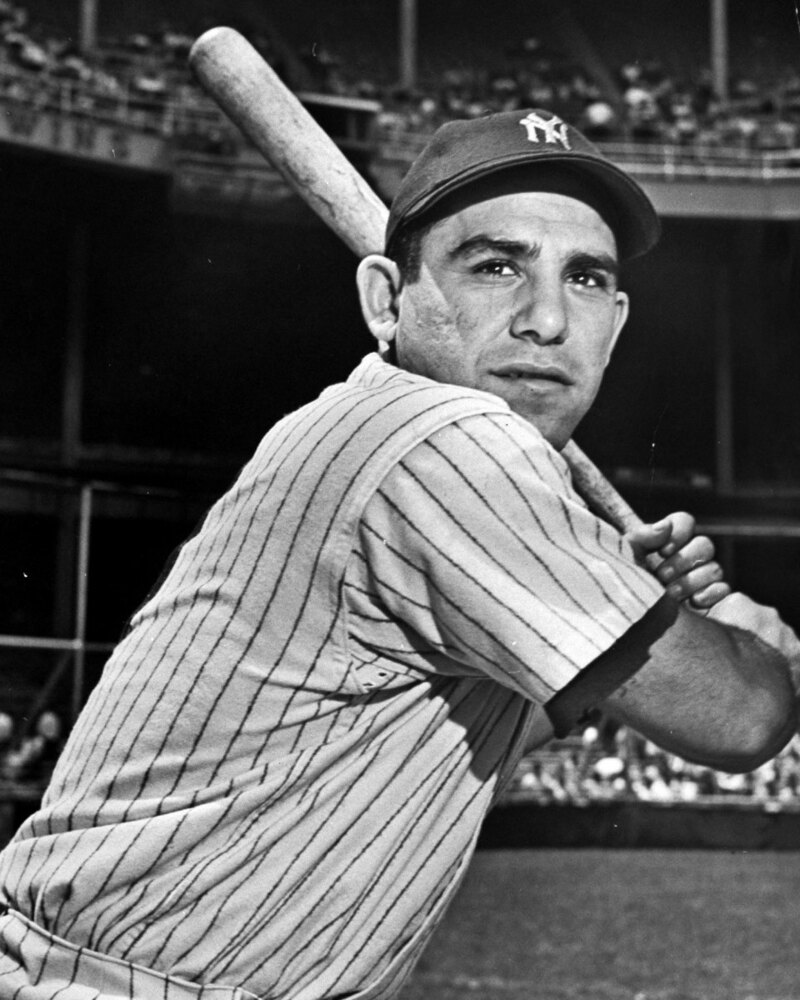
\includegraphics[max width=0.95\textwidth,
        max height=0.58000\textheight]{{Images/berra}.jpg}
    \end{center}
    \end{column}
    \end{columns}
}
\end{frame}
\begin{frame}[t]{Round 1 --- Quotations --- \mbox{Answer 4}}
\vspace{-0.5em}
\begin{block}{Question}
``Be the change that you wish to see in the world.''
\end{block}

\visible<2->{
    \begin{columns}[T,totalwidth=\linewidth]
    \begin{column}{0.32\linewidth}
    \begin{block}{Answer}
    Mahatma Gandhi
    \end{block}
    \end{column}
    \begin{column}{0.65\linewidth}
    \begin{center}
    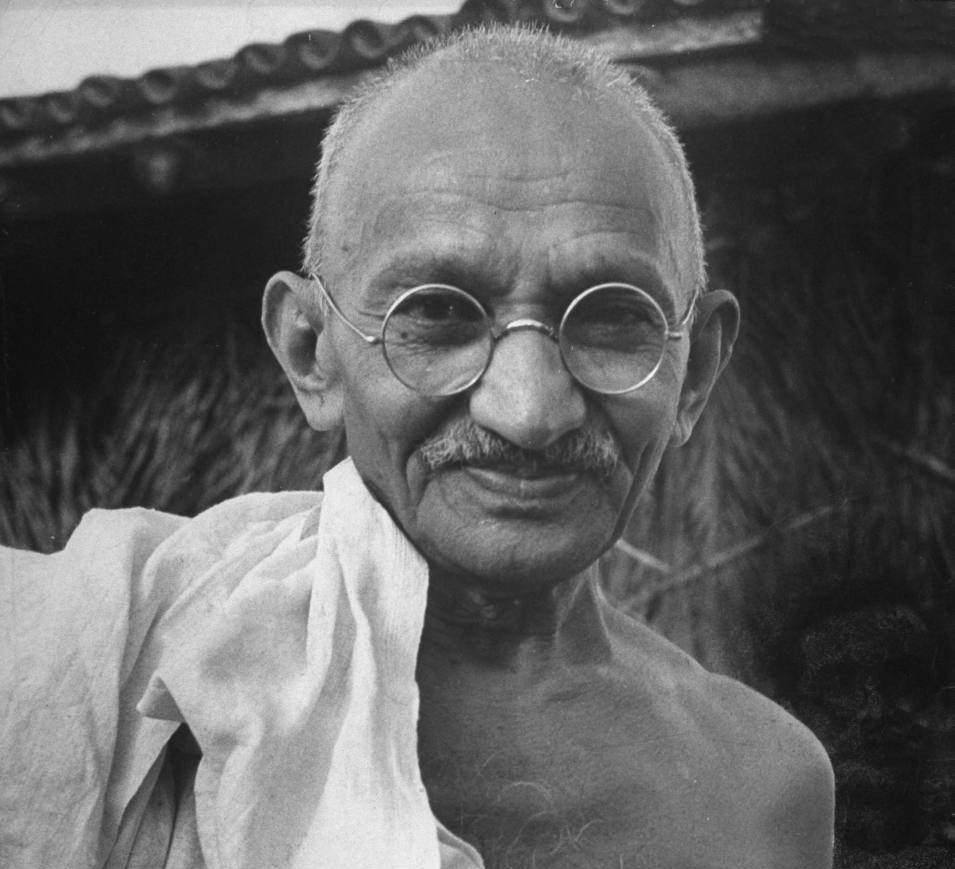
\includegraphics[max width=0.95\textwidth,
        max height=0.54000\textheight]{{Images/gandhi}.jpg}
    \end{center}
    \end{column}
    \end{columns}
}
\end{frame}
\begin{frame}[t]{Round 1 --- Quotations --- \mbox{Answer 5}}
\vspace{-0.5em}
\begin{block}{Question}
``The reports of my death are greatly exaggerated.''
\end{block}

\visible<2->{
    \begin{columns}[T,totalwidth=\linewidth]
    \begin{column}{0.32\linewidth}
    \begin{block}{Answer}
    Mark Twain
    \end{block}
    \end{column}
    \begin{column}{0.65\linewidth}
    \begin{center}
    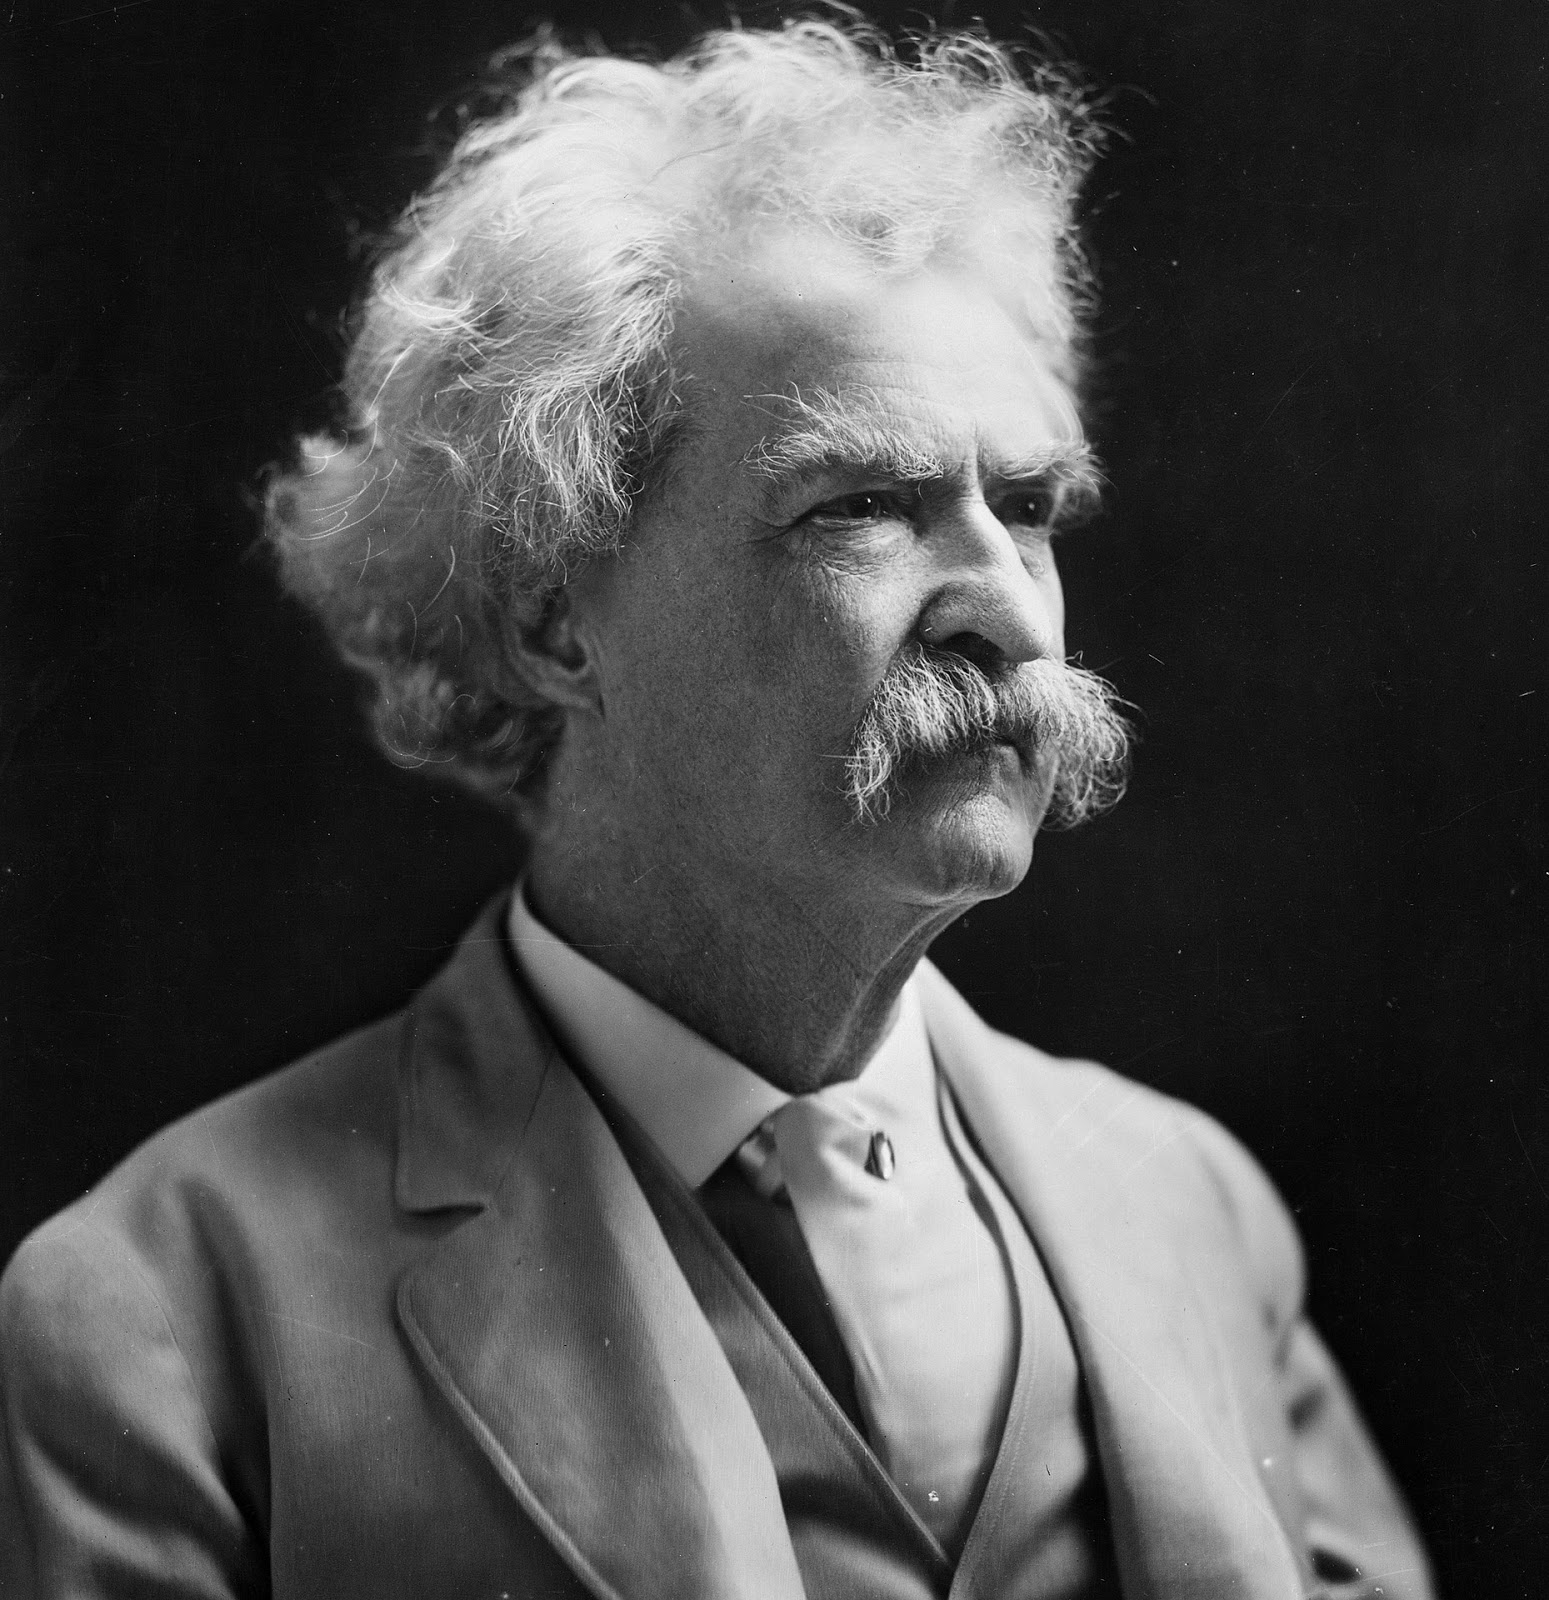
\includegraphics[max width=0.95\textwidth,
        max height=0.54000\textheight]{{Images/twain}.jpg}
    \end{center}
    \end{column}
    \end{columns}
}
\end{frame}
\begin{frame}[t]{Round 1 --- Quotations --- \mbox{Answer 6}}
\vspace{-0.5em}
\begin{block}{Question}
``I am the straw that stirs the drink'' has been attributed to which athlete (who has denied saying it)?
\end{block}

\visible<2->{
    \begin{columns}[T,totalwidth=\linewidth]
    \begin{column}{0.32\linewidth}
    \begin{block}{Answer}
    Reggie Jackson
    \end{block}
    \end{column}
    \begin{column}{0.65\linewidth}
    \begin{center}
    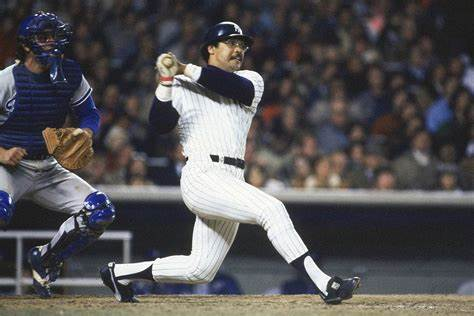
\includegraphics[max width=0.95\textwidth,
        max height=0.50000\textheight]{{Images/reggie}.jpeg}
    \end{center}
    \end{column}
    \end{columns}
}
\end{frame}
\begin{frame}[t]{Round 1 --- Quotations --- \mbox{Answer 7}}
\vspace{-0.5em}
\begin{block}{Question}
``Always forgive your enemies; nothing annoys them so much.''
\end{block}

\visible<2->{
    \begin{columns}[T,totalwidth=\linewidth]
    \begin{column}{0.32\linewidth}
    \begin{block}{Answer}
    Oscar Wilde
    \end{block}
    \end{column}
    \begin{column}{0.65\linewidth}
    \begin{center}
    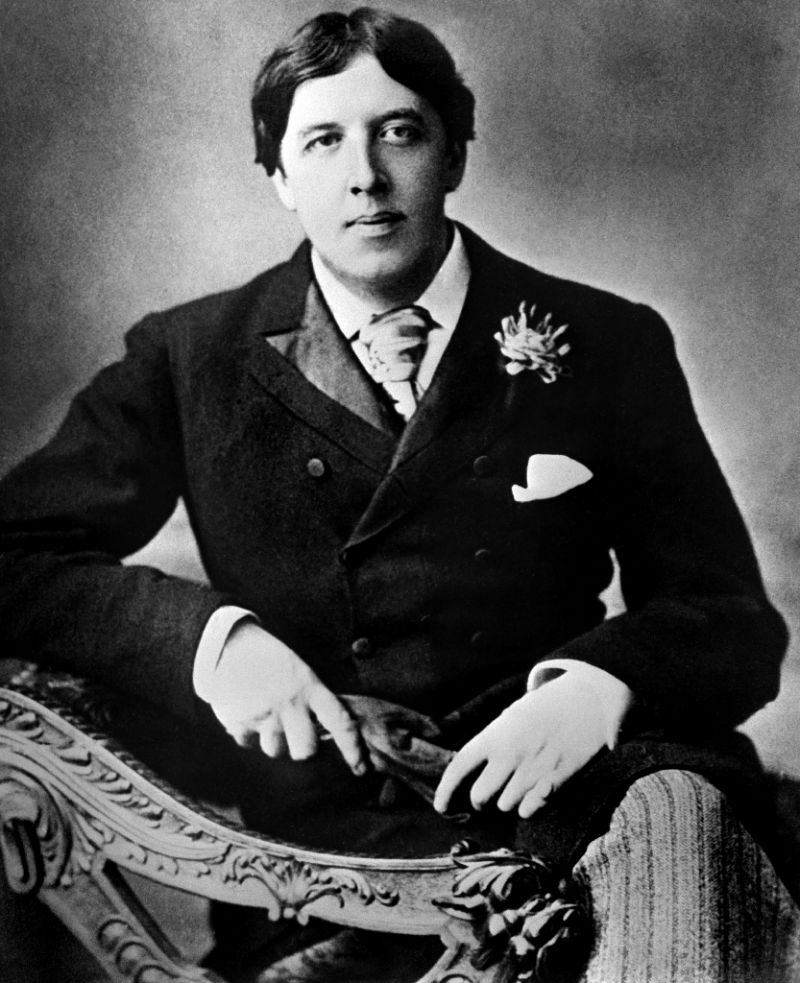
\includegraphics[max width=0.95\textwidth,
        max height=0.54000\textheight]{{Images/wilde}.jpg}
    \end{center}
    \end{column}
    \end{columns}
}
\end{frame}
\begin{frame}[t]{Round 1 --- Quotations --- \mbox{Answer 8}}
\vspace{-0.5em}
\begin{block}{Question}
``When you are courting a nice girl an hour seems like a second. When you sit on a red-hot cinder a second seems like an hour.''
\end{block}

\visible<2->{
    \begin{columns}[T,totalwidth=\linewidth]
    \begin{column}{0.32\linewidth}
    \begin{block}{Answer}
    Albert Einstein (on relativity)
    \end{block}
    \end{column}
    \begin{column}{0.65\linewidth}
    \begin{center}
    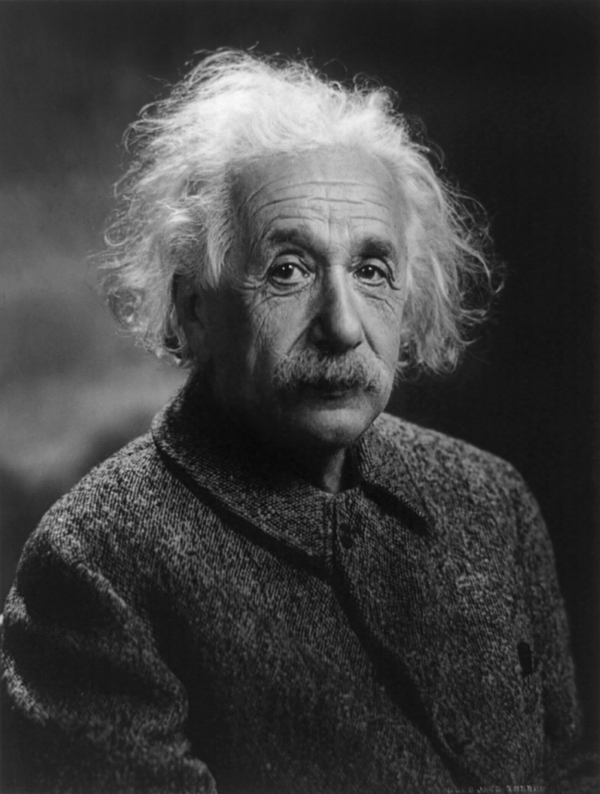
\includegraphics[max width=0.95\textwidth,
        max height=0.50000\textheight]{{Images/einstein}.jpg}
    \end{center}
    \end{column}
    \end{columns}
}
\end{frame}
\begin{frame}[t]{Round 1 --- Quotations --- \mbox{Answer 9}}
\vspace{-0.5em}
\begin{block}{Question}
``If I were two-faced, would I be wearing this one?''
\end{block}

\visible<2->{
    \begin{columns}[T,totalwidth=\linewidth]
    \begin{column}{0.32\linewidth}
    \begin{block}{Answer}
    Abraham Lincoln
    \end{block}
    \end{column}
    \begin{column}{0.65\linewidth}
    \begin{center}
    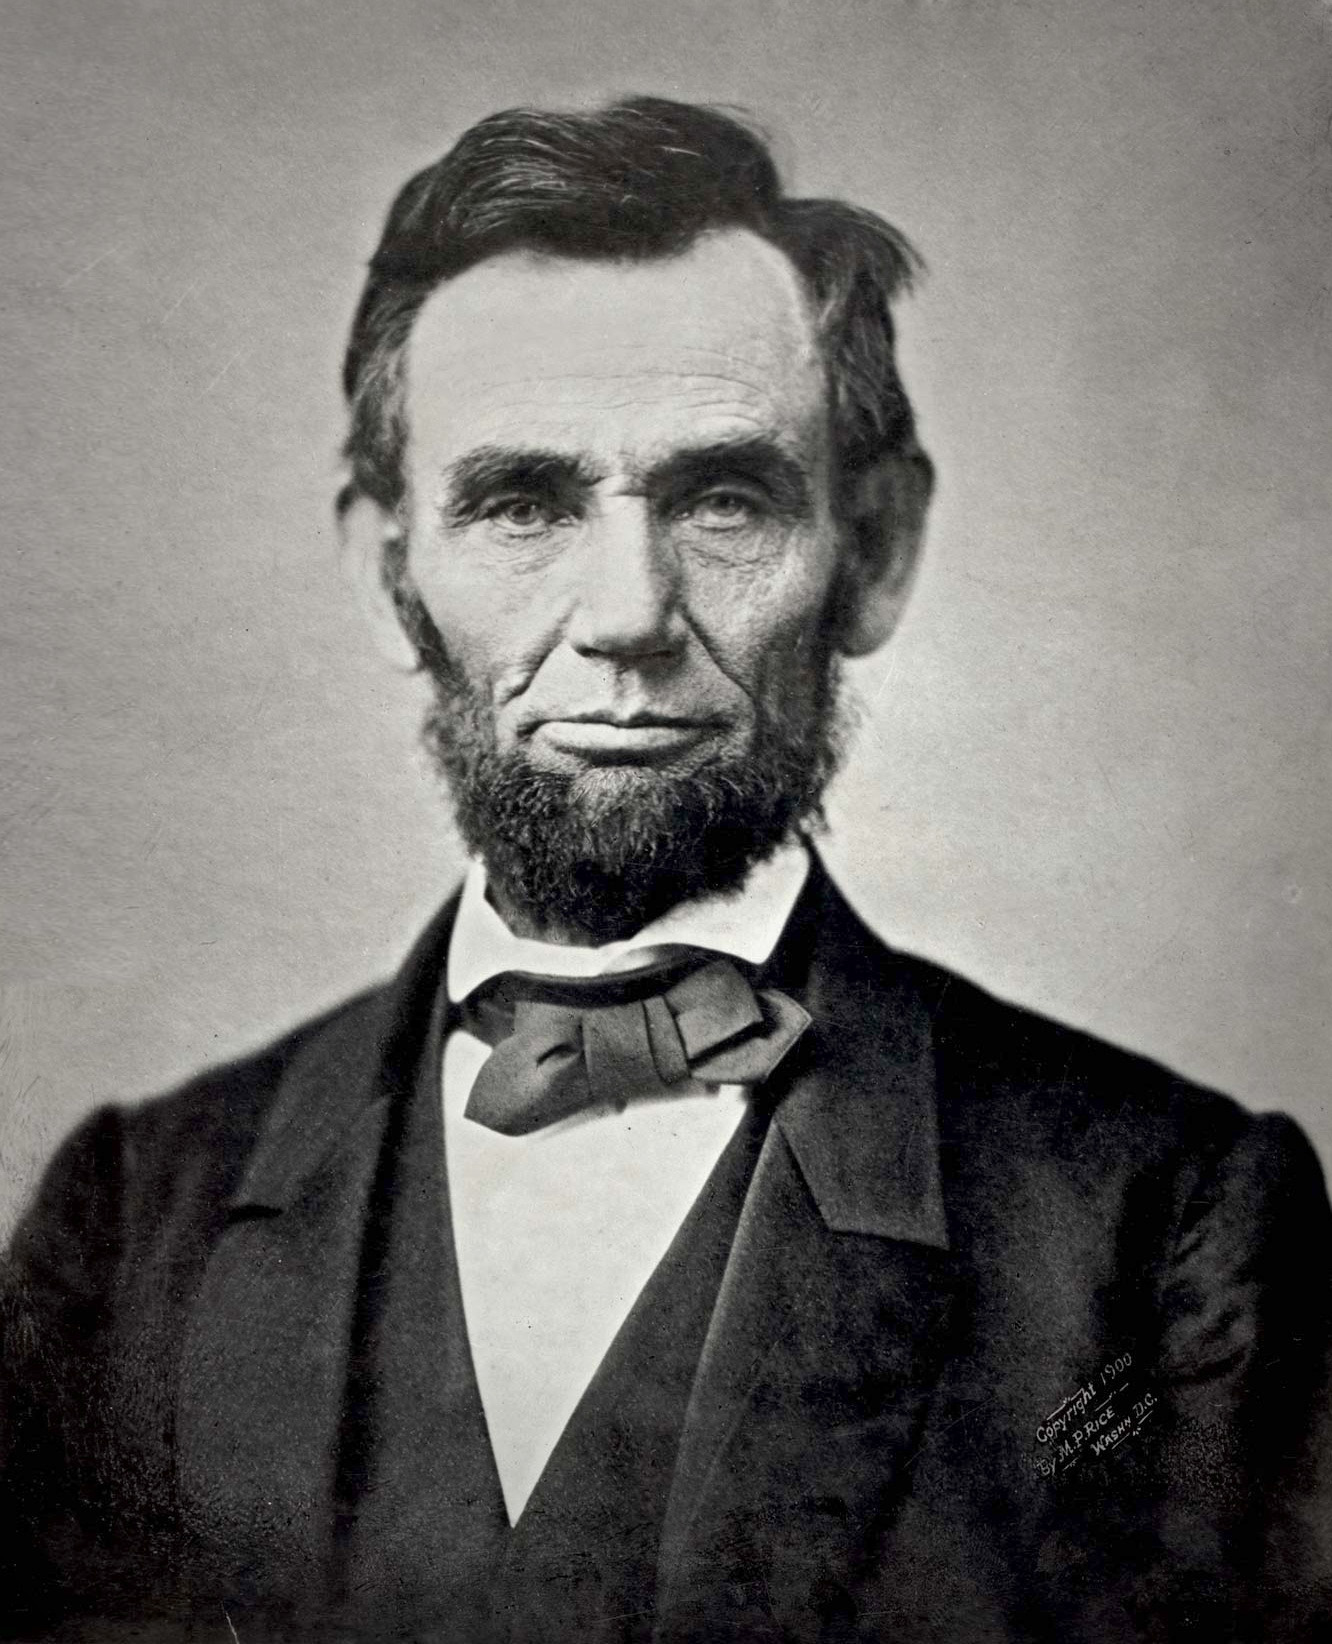
\includegraphics[max width=0.95\textwidth,
        max height=0.54000\textheight]{{Images/lincoln}.jpg}
    \end{center}
    \end{column}
    \end{columns}
}
\end{frame}
\begin{frame}[t]{Round 1 --- Quotations --- \mbox{Answer 10}}
\vspace{-0.5em}
\begin{block}{Question}
Which Shakespeare character says, ``If you prick us, do we not bleed? If you tickle us, do we not laugh?''
\end{block}

\visible<2->{
    \begin{columns}[T,totalwidth=\linewidth]
    \begin{column}{0.32\linewidth}
    \begin{block}{Answer}
    Shylock (in \emph{The Merchant of Venice})
    \end{block}
    \end{column}
    \begin{column}{0.65\linewidth}
    \begin{center}
    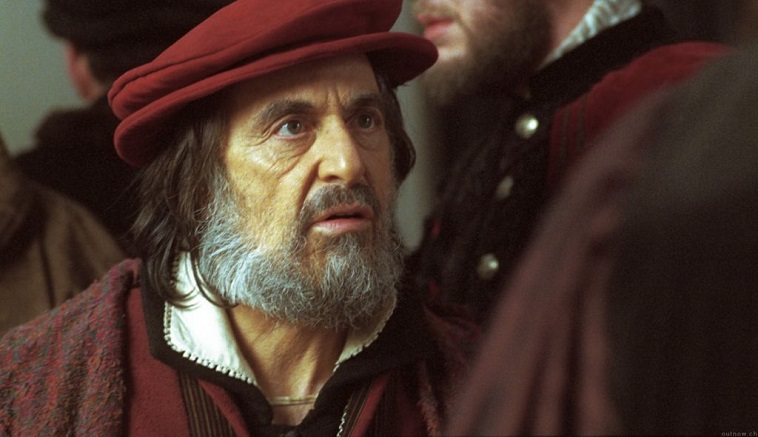
\includegraphics[max width=0.95\textwidth,
        max height=0.50000\textheight]{{Images/shylock}.jpg}
    \end{center}
    \end{column}
    \end{columns}
}
\end{frame}
\def\thisSectionName{East Asia}
\section{Round 2}
\subsection*{Q1}
\begin{frame}[t]{Round 2 --- East Asia --- \mbox{Question 1}}
\vspace{-0.5em}
\begin{block}{Question}
What is the name of the Vietnamese Lunar New Year?
\end{block}
\end{frame}
\subsection*{Q2}
\begin{frame}[t]{Round 2 --- East Asia --- \mbox{Question 2}}
\vspace{-0.5em}
\begin{columns}[T,totalwidth=\linewidth]
\begin{column}{0.32\linewidth}
\begin{block}{Question}
Pictured here (the golden spires) is the oldest Buddhist pagoda in the world.  In which country is it located?
\end{block}
\end{column}
\begin{column}{0.65\linewidth}
\begin{center}
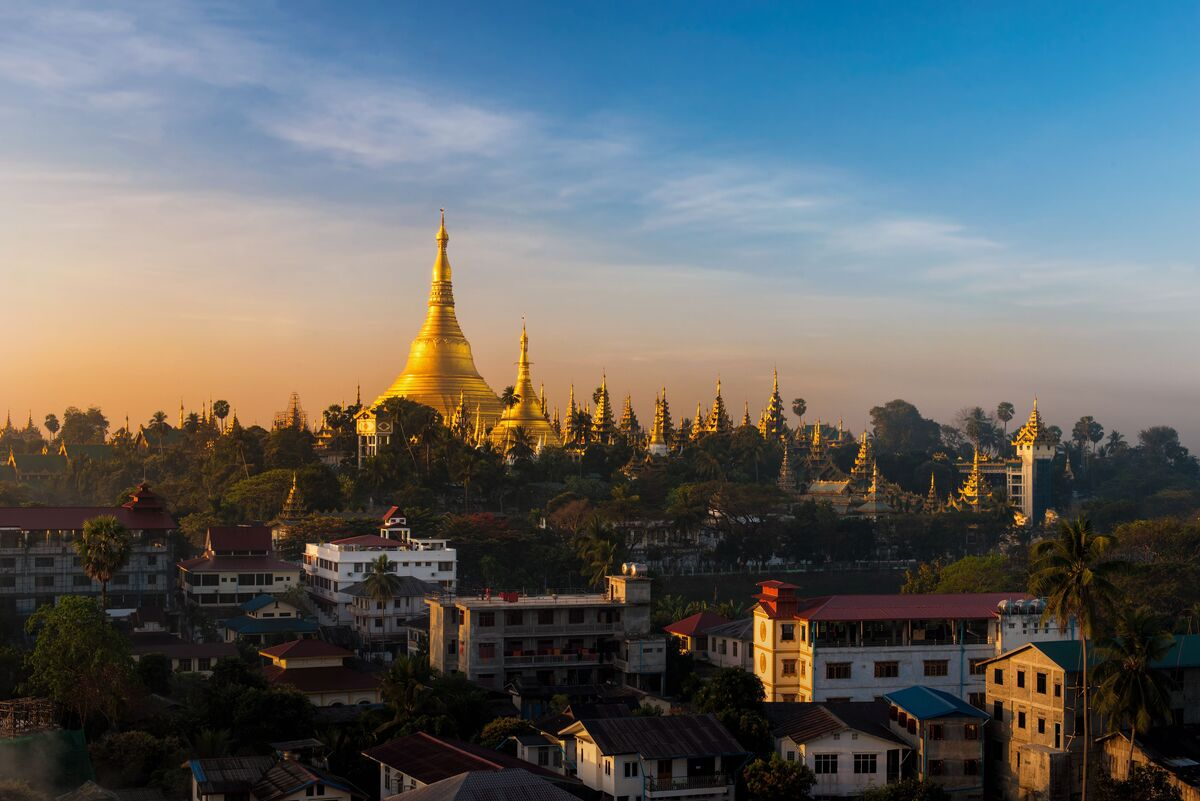
\includegraphics[max width=0.95\textwidth,max height=0.7\textheight]{{Images/yangon}.jpg}
\end{center}
\end{column}
\end{columns}
\end{frame}
\subsection*{Q3}
\begin{frame}[t]{Round 2 --- East Asia --- \mbox{Question 3}}
\vspace{-0.5em}
\begin{block}{Question}
What is the capital of Laos?
\end{block}
\end{frame}
\subsection*{Q4}
\begin{frame}[t]{Round 2 --- East Asia --- \mbox{Question 4}}
\vspace{-0.5em}
\begin{block}{Question}
By population, which Asian metropolitan area is the largest metropolitan area in the world?
\end{block}
\end{frame}
\subsection*{Q5}
\begin{frame}[t]{Round 2 --- East Asia --- \mbox{Question 5}}
\vspace{-0.5em}
\begin{block}{Question}
In Japan, food from which chain has become a popular Christmas Eve dinner, with customers placing orders weeks in advance to avoid missing out?
\end{block}
\end{frame}
\subsection*{Q6}
\begin{frame}[t]{Round 2 --- East Asia --- \mbox{Question 6}}
\vspace{-0.5em}
\begin{columns}[T,totalwidth=\linewidth]
\begin{column}{0.32\linewidth}
\begin{block}{Question}
Which country or region's flag is pictured here?
\end{block}
\end{column}
\begin{column}{0.65\linewidth}
\begin{center}
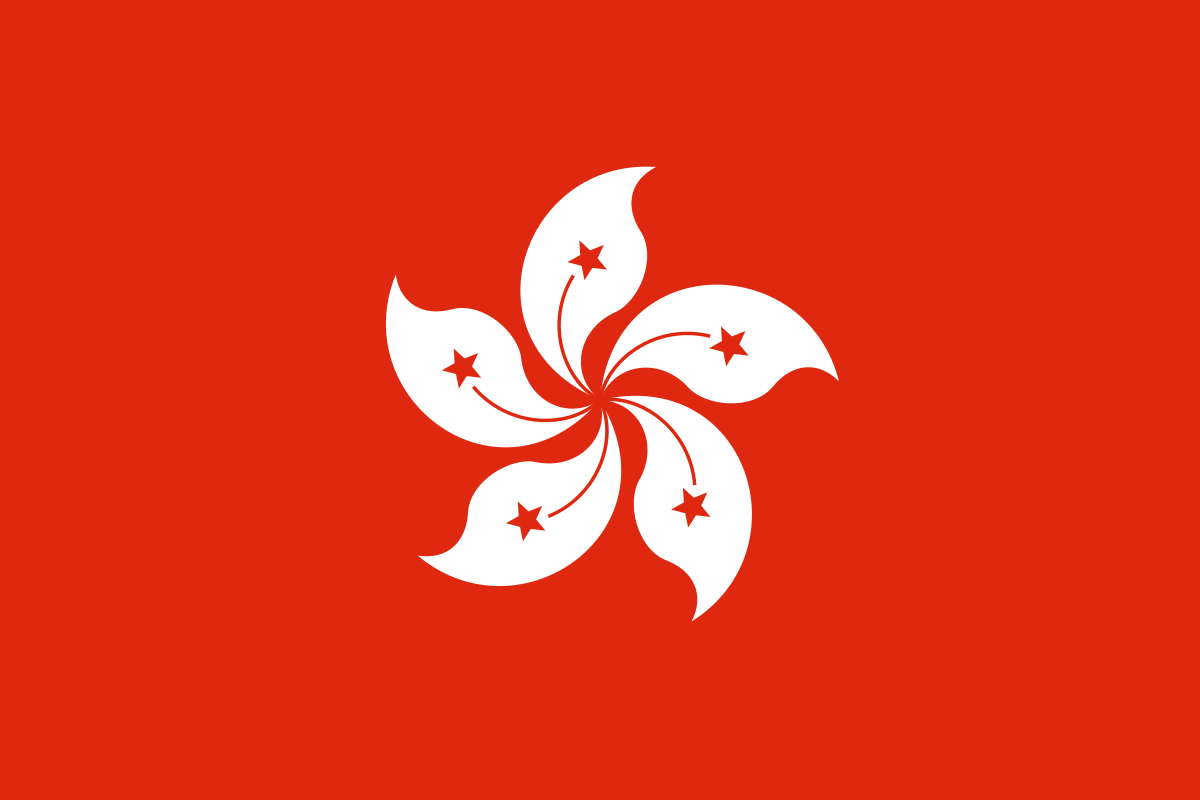
\includegraphics[max width=0.95\textwidth,max height=0.7\textheight]{{Images/hongkong}.png}
\end{center}
\end{column}
\end{columns}
\end{frame}
\subsection*{Q7}
\begin{frame}[t]{Round 2 --- East Asia --- \mbox{Question 7}}
\vspace{-0.5em}
\begin{block}{Question}
How many time zones does China officially have?
\end{block}
\end{frame}
\subsection*{Q8}
\begin{frame}[t]{Round 2 --- East Asia --- \mbox{Question 8}}
\vspace{-0.5em}
\begin{block}{Question}
Angkor Wat in Cambodia was originally constructed as a temple for which religion?
\end{block}
\end{frame}
\subsection*{Q9}
\begin{frame}[t]{Round 2 --- East Asia --- \mbox{Question 9}}
\vspace{-0.5em}
\begin{block}{Question}
What was the name of the network of trade routes that spanned Asia and connected the East and the West, and which Marco Polo traveled along on his famous journey?
\end{block}
\end{frame}
\subsection*{Q10}
\begin{frame}[t]{Round 2 --- East Asia --- \mbox{Question 10}}
\vspace{-0.5em}
\begin{columns}[T,totalwidth=\linewidth]
\begin{column}{0.32\linewidth}
\begin{block}{Question}
What is the name of the traditional Mongolian tent pictured here?
\end{block}
\end{column}
\begin{column}{0.65\linewidth}
\begin{center}
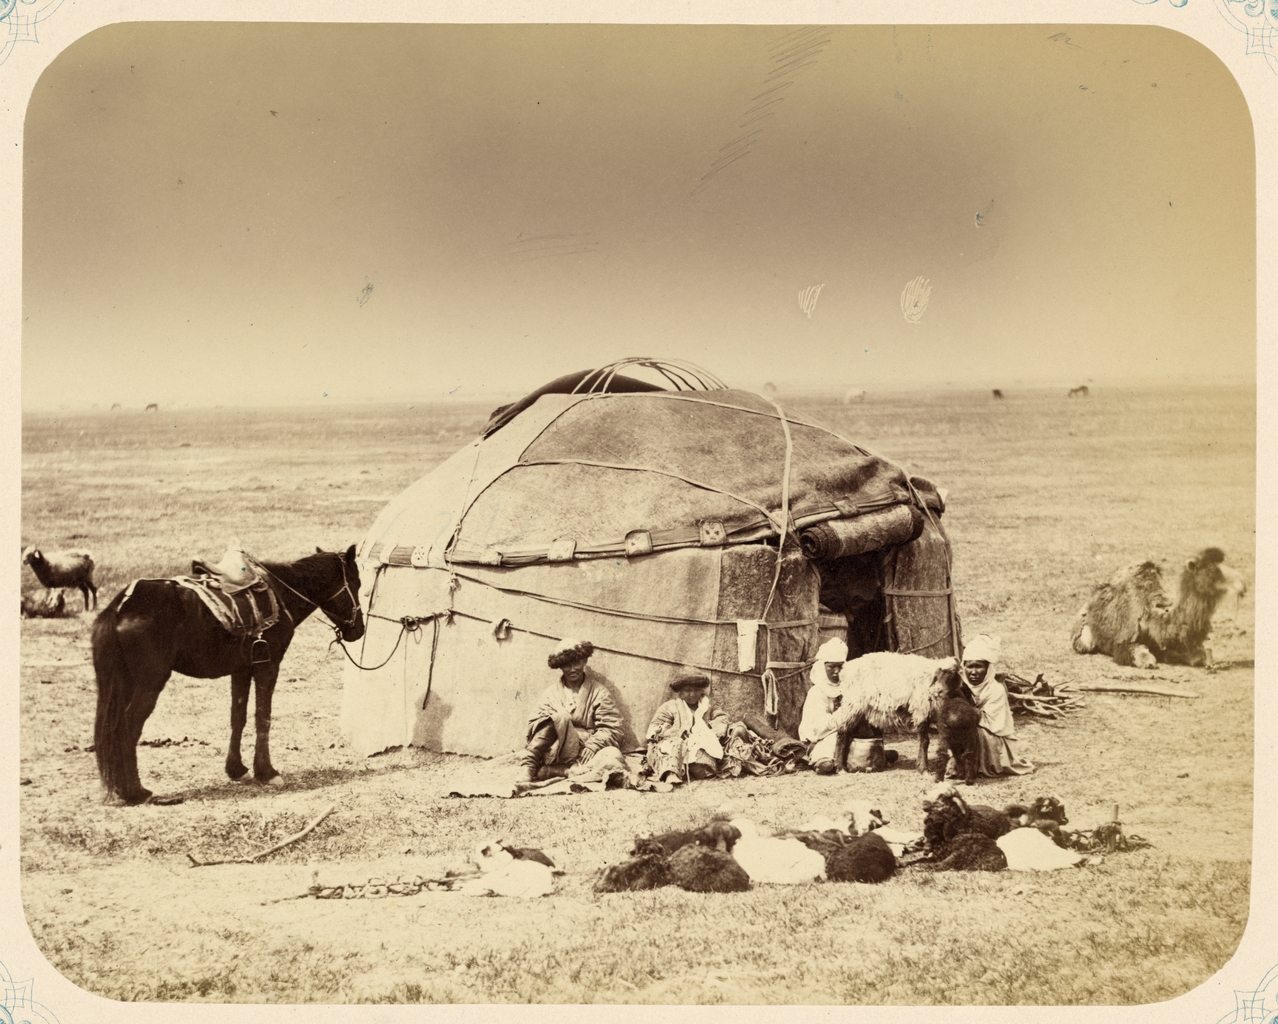
\includegraphics[max width=0.95\textwidth,max height=0.7\textheight]{{Images/yurt}.png}
\end{center}
\end{column}
\end{columns}
\end{frame}
\subsection{Answers}
\begin{frame}[t]{Round 2 --- East Asia --- \mbox{Answer 1}}
\vspace{-0.5em}
\begin{block}{Question}
What is the name of the Vietnamese Lunar New Year?
\end{block}

\visible<2->{
    \begin{columns}[T,totalwidth=\linewidth]
    \begin{column}{0.32\linewidth}
    \begin{block}{Answer}
    T\'{\^{e}}t
    \end{block}
    \end{column}
    \begin{column}{0.65\linewidth}
    \begin{center}
    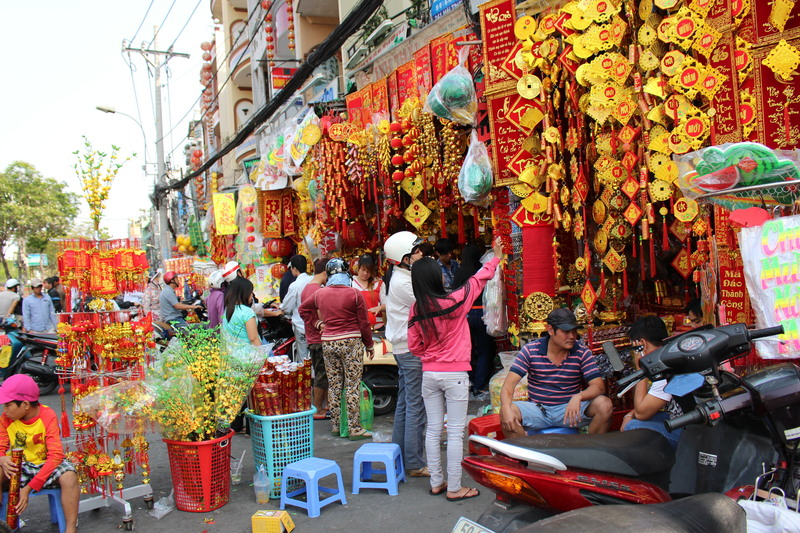
\includegraphics[max width=0.95\textwidth,
        max height=0.58000\textheight]{{Images/tetviet}.jpg}
    \end{center}
    \end{column}
    \end{columns}
}
\end{frame}
\begin{frame}[t]{Round 2 --- East Asia --- \mbox{Answer 2}}
\vspace{-0.5em}
\begin{columns}[T,totalwidth=\linewidth]
\begin{column}{0.32\linewidth}
\begin{block}{Question}
Pictured here (the golden spires) is the oldest Buddhist pagoda in the world.  In which country is it located?
\end{block}
\visible<2->{
    \begin{block}{Answer}
    Myanmar
    \end{block}
}
\end{column}
\begin{column}{0.65\linewidth}
\begin{center}
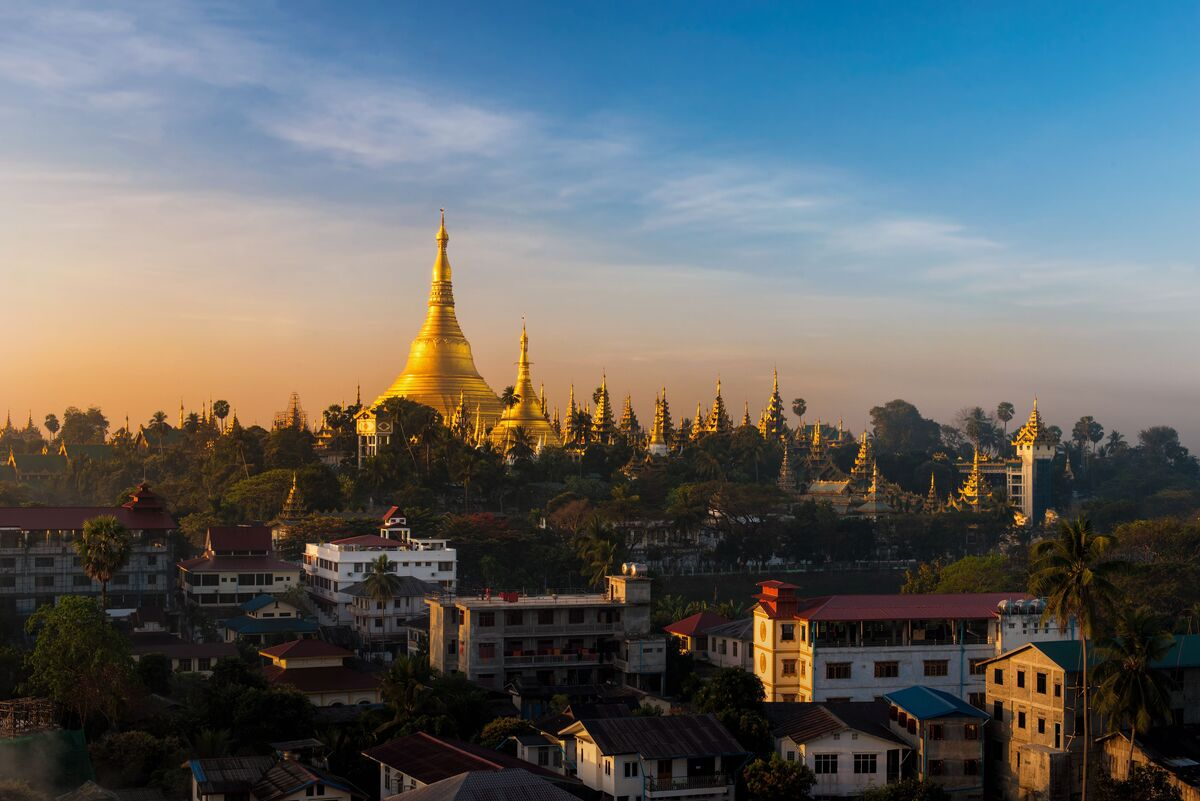
\includegraphics[max width=0.95\textwidth,max height=0.7\textheight]{{Images/yangon}.jpg}
\end{center}
\end{column}
\end{columns}
\end{frame}
\begin{frame}[t]{Round 2 --- East Asia --- \mbox{Answer 3}}
\vspace{-0.5em}
\begin{block}{Question}
What is the capital of Laos?
\end{block}

\visible<2->{
    \begin{columns}[T,totalwidth=\linewidth]
    \begin{column}{0.32\linewidth}
    \begin{block}{Answer}
    Vientiane
    \end{block}
    \end{column}
    \begin{column}{0.65\linewidth}
    \begin{center}
    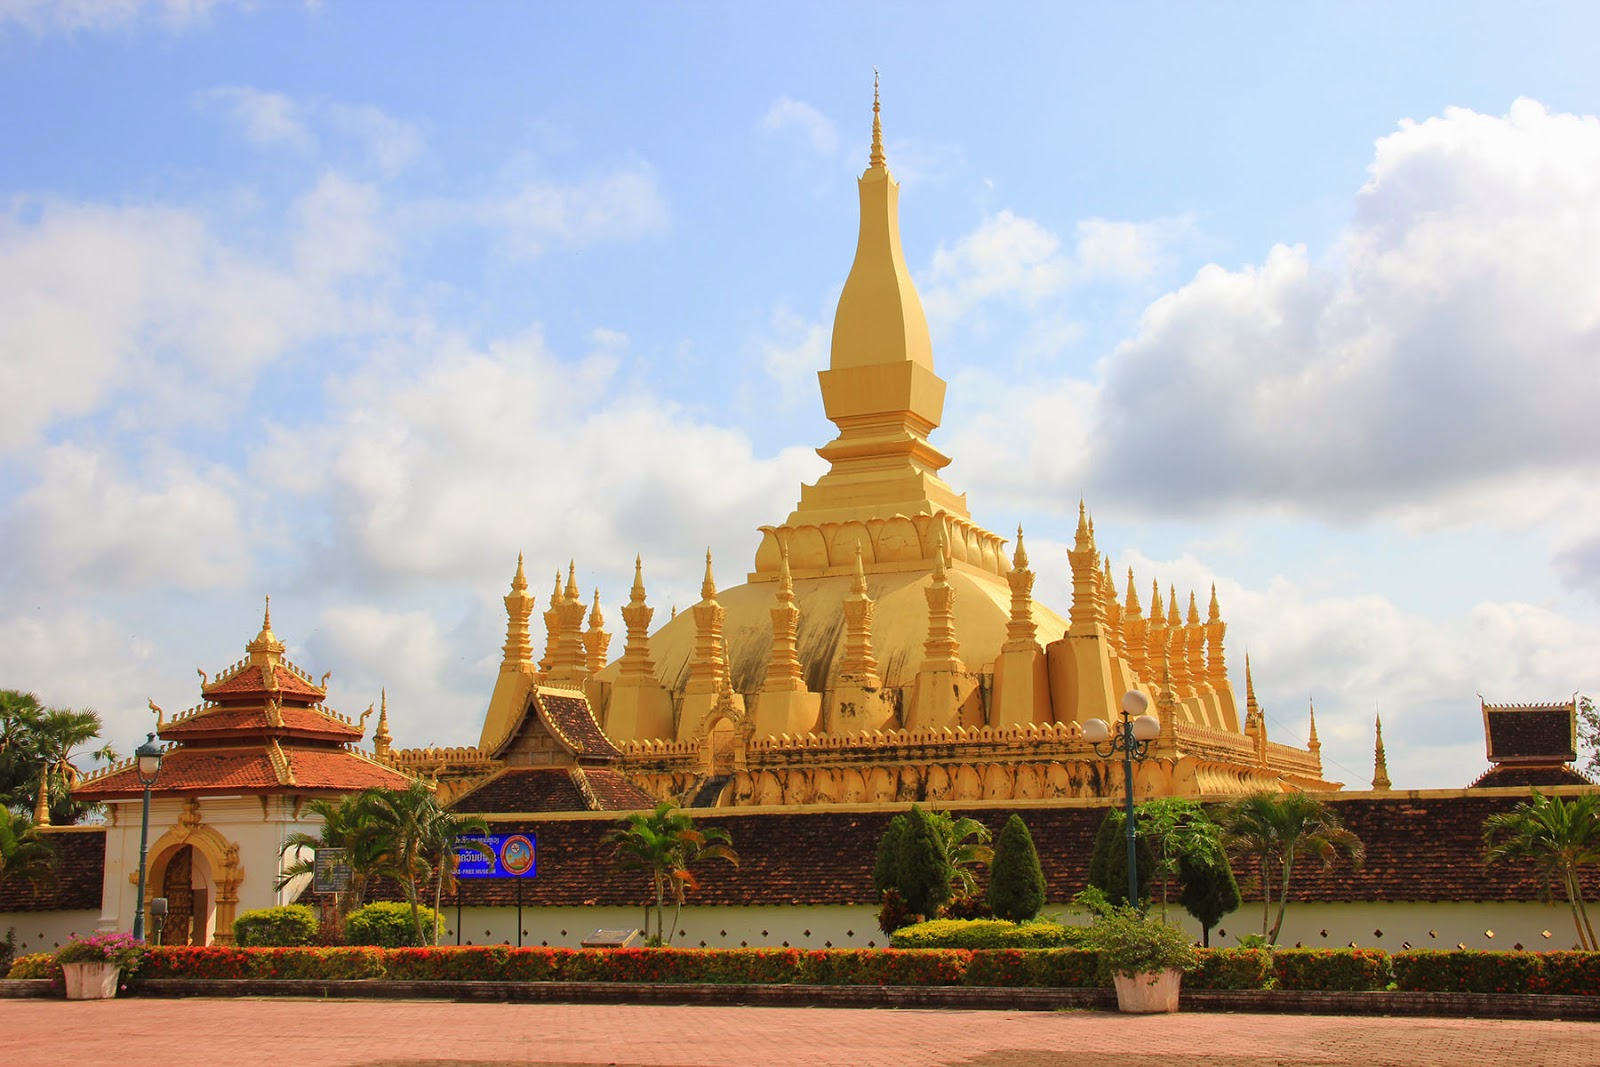
\includegraphics[max width=0.95\textwidth,
        max height=0.58000\textheight]{{Images/vientiane}.jpg}
    \end{center}
    \end{column}
    \end{columns}
}
\end{frame}
\begin{frame}[t]{Round 2 --- East Asia --- \mbox{Answer 4}}
\vspace{-0.5em}
\begin{block}{Question}
By population, which Asian metropolitan area is the largest metropolitan area in the world?
\end{block}

\visible<2->{
    \begin{columns}[T,totalwidth=\linewidth]
    \begin{column}{0.32\linewidth}
    \begin{block}{Answer}
    The Tokyo metropolitan area (33 million people)
    \end{block}
    \end{column}
    \begin{column}{0.65\linewidth}
    \begin{center}
    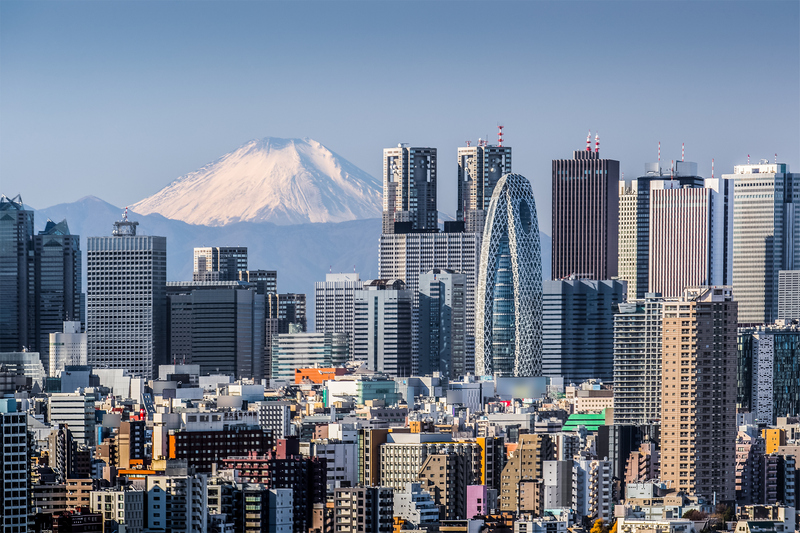
\includegraphics[max width=0.95\textwidth,
        max height=0.54000\textheight]{{Images/tokyo}.jpg}
    \end{center}
    \end{column}
    \end{columns}
}
\end{frame}
\begin{frame}[t]{Round 2 --- East Asia --- \mbox{Answer 5}}
\vspace{-0.5em}
\begin{block}{Question}
In Japan, food from which chain has become a popular Christmas Eve dinner, with customers placing orders weeks in advance to avoid missing out?
\end{block}

\visible<2->{
    \begin{columns}[T,totalwidth=\linewidth]
    \begin{column}{0.32\linewidth}
    \begin{block}{Answer}
    Kentucky Fried Chicken
    \end{block}
    \end{column}
    \begin{column}{0.65\linewidth}
    \begin{center}
    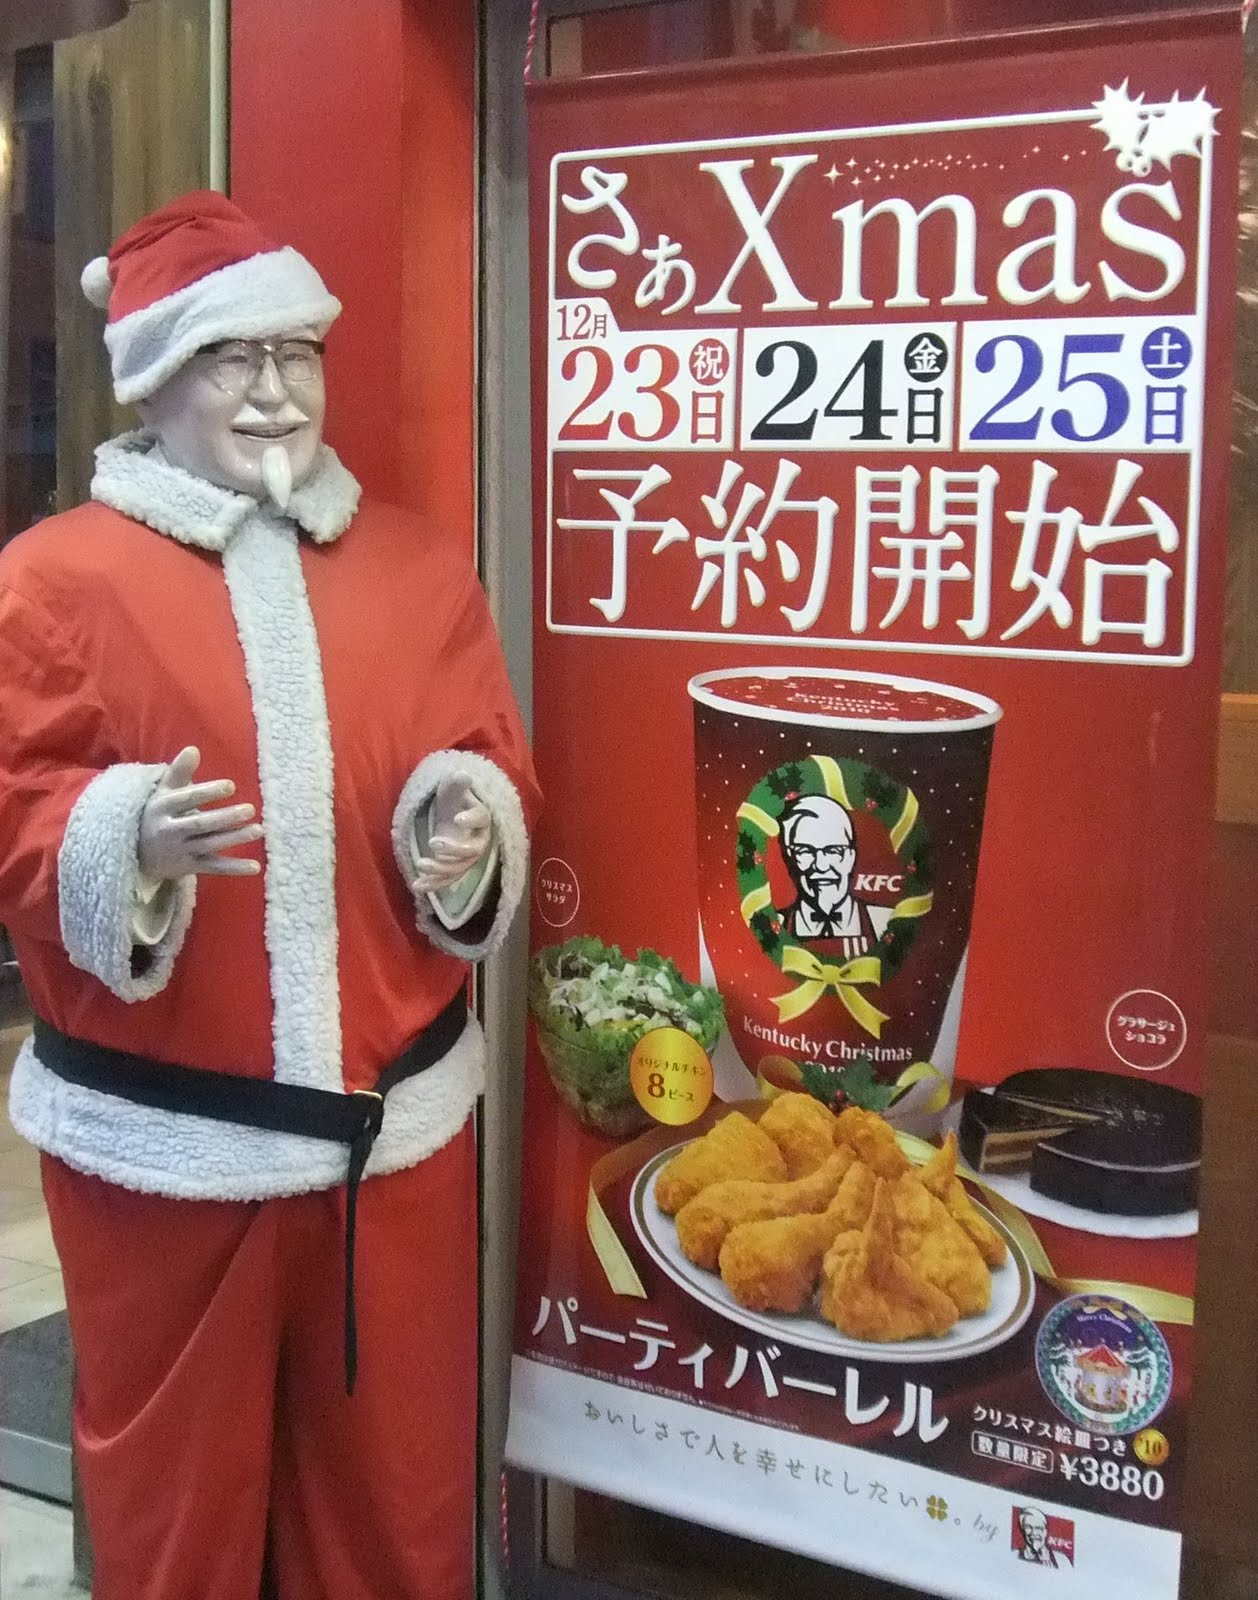
\includegraphics[max width=0.95\textwidth,
        max height=0.50000\textheight]{{Images/kfc}.jpg}
    \end{center}
    \end{column}
    \end{columns}
}
\end{frame}
\begin{frame}[t]{Round 2 --- East Asia --- \mbox{Answer 6}}
\vspace{-0.5em}
\begin{columns}[T,totalwidth=\linewidth]
\begin{column}{0.38\linewidth}
\begin{block}{Question}
Which country or region's flag is pictured here?
\end{block}
\end{column}
\begin{column}{0.6\linewidth}
\begin{center}
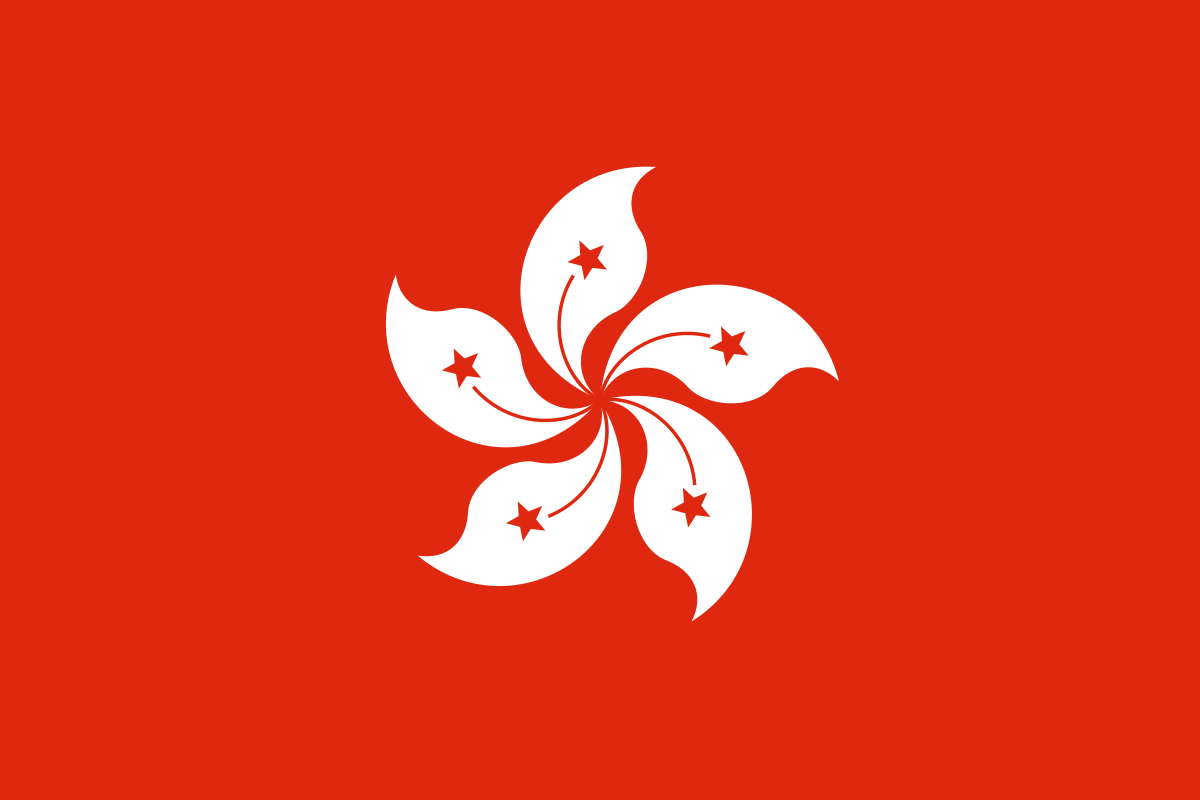
\includegraphics[max width=0.95\textwidth,max height=0.35\textheight]{{Images/hongkong}.png}
\end{center}
\end{column}
\end{columns}

\visible<2->{
    \begin{columns}[T,totalwidth=\linewidth]
    \begin{column}{0.38\linewidth}
    \begin{block}{Answer}
    Hong Kong
    \end{block}
    \end{column}
    \begin{column}{0.6\linewidth}
    \begin{center}
    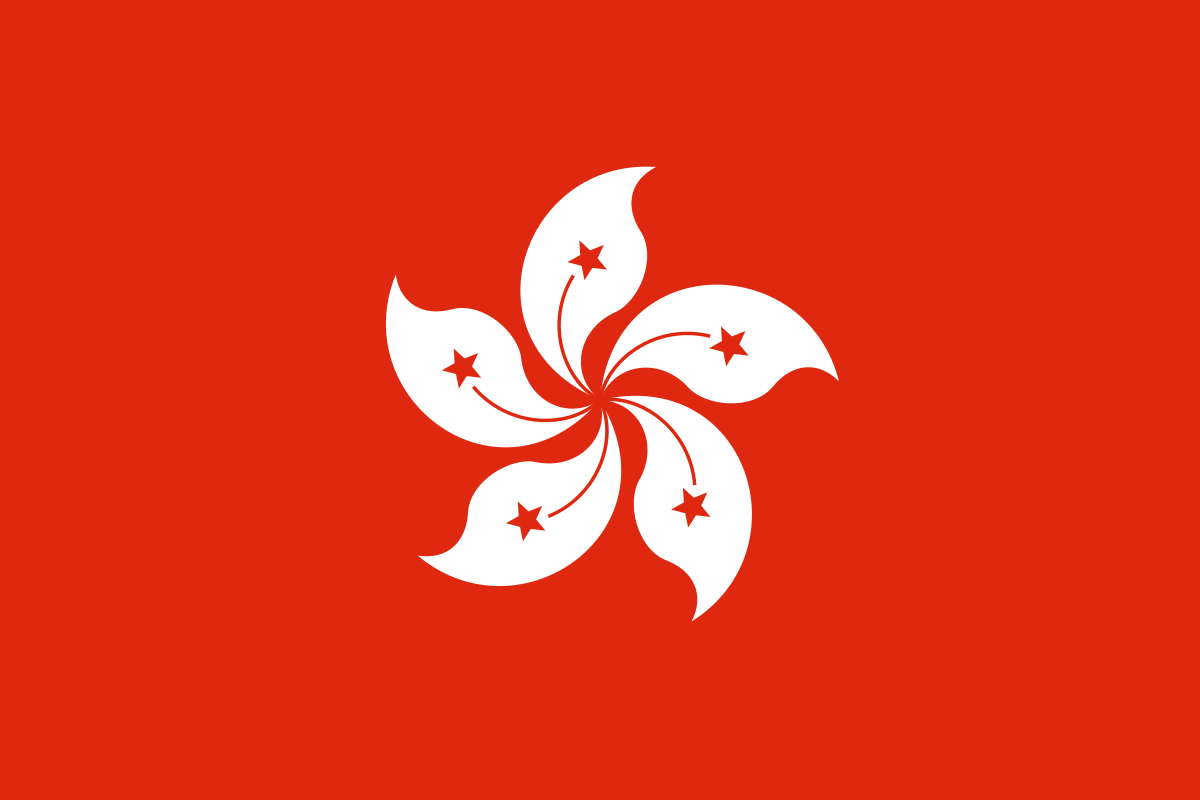
\includegraphics[max width=0.95\textwidth,
        max height=0.34\textheight]{{Images/hongkong}.jpg}
    \end{center}
    \end{column}
    \end{columns}
}
\end{frame}
\begin{frame}[t]{Round 2 --- East Asia --- \mbox{Answer 7}}
\vspace{-0.5em}
\begin{block}{Question}
How many time zones does China officially have?
\end{block}

\visible<2->{
    \begin{columns}[T,totalwidth=\linewidth]
    \begin{column}{0.32\linewidth}
    \begin{block}{Answer}
    One
    \end{block}
    \end{column}
    \begin{column}{0.65\linewidth}
    \begin{center}
    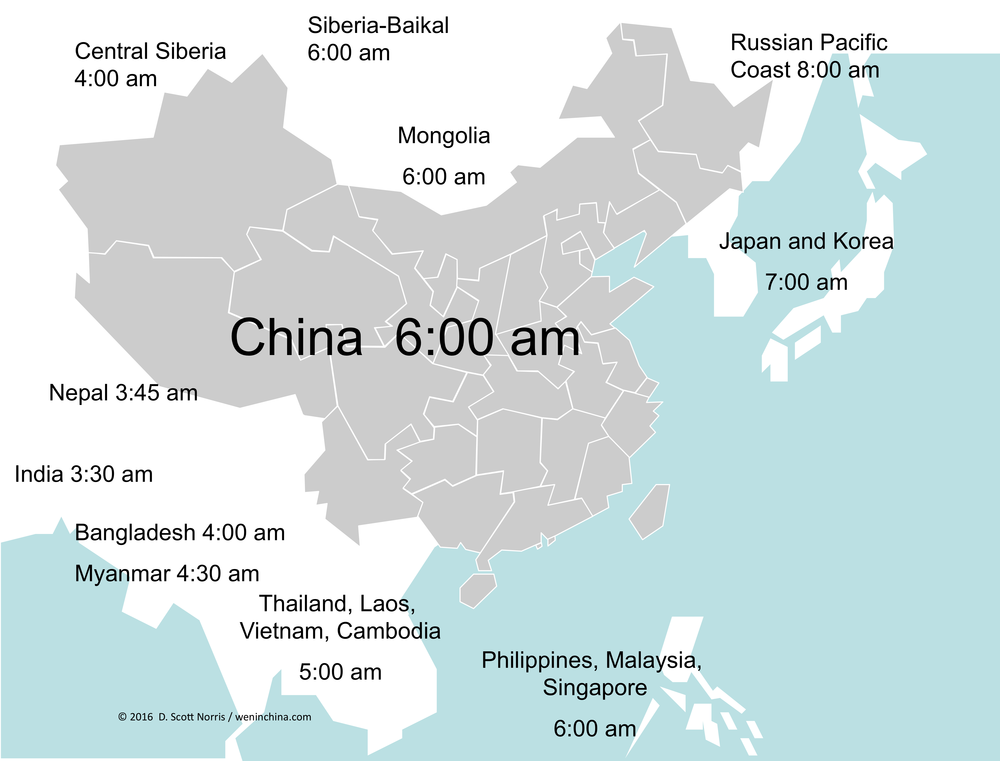
\includegraphics[max width=0.95\textwidth,
        max height=0.58000\textheight]{{Images/chinatime}.png}
    \end{center}
    \end{column}
    \end{columns}
}
\end{frame}
\begin{frame}[t]{Round 2 --- East Asia --- \mbox{Answer 8}}
\vspace{-0.5em}
\begin{block}{Question}
Angkor Wat in Cambodia was originally constructed as a temple for which religion?
\end{block}

\visible<2->{
    \begin{columns}[T,totalwidth=\linewidth]
    \begin{column}{0.32\linewidth}
    \begin{block}{Answer}
    Hinduism
    \end{block}
    \end{column}
    \begin{column}{0.65\linewidth}
    \begin{center}
    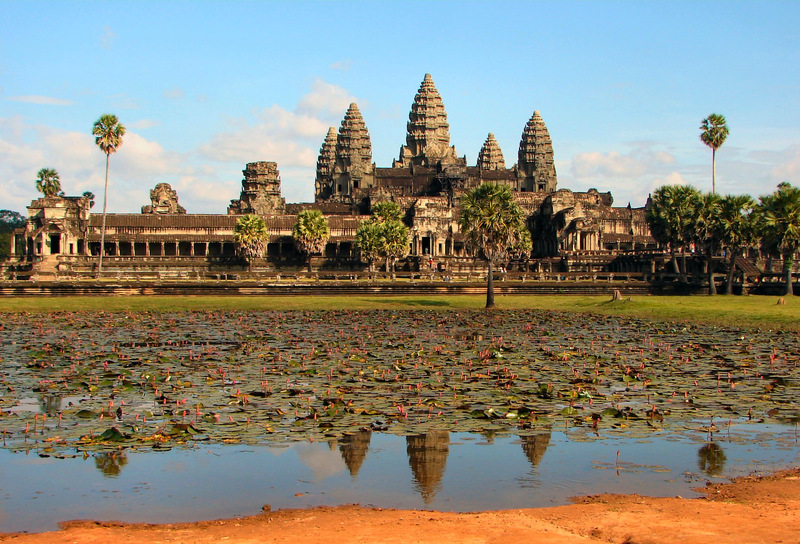
\includegraphics[max width=0.95\textwidth,
        max height=0.54000\textheight]{{Images/angkor}.jpg}
    \end{center}
    \end{column}
    \end{columns}
}
\end{frame}
\begin{frame}[t]{Round 2 --- East Asia --- \mbox{Answer 9}}
\vspace{-0.5em}
\begin{block}{Question}
What was the name of the network of trade routes that spanned Asia and connected the East and the West, and which Marco Polo traveled along on his famous journey?
\end{block}

\visible<2->{
    \begin{columns}[T,totalwidth=\linewidth]
    \begin{column}{0.32\linewidth}
    \begin{block}{Answer}
    The Silk Road
    \end{block}
    \end{column}
    \begin{column}{0.65\linewidth}
    \begin{center}
    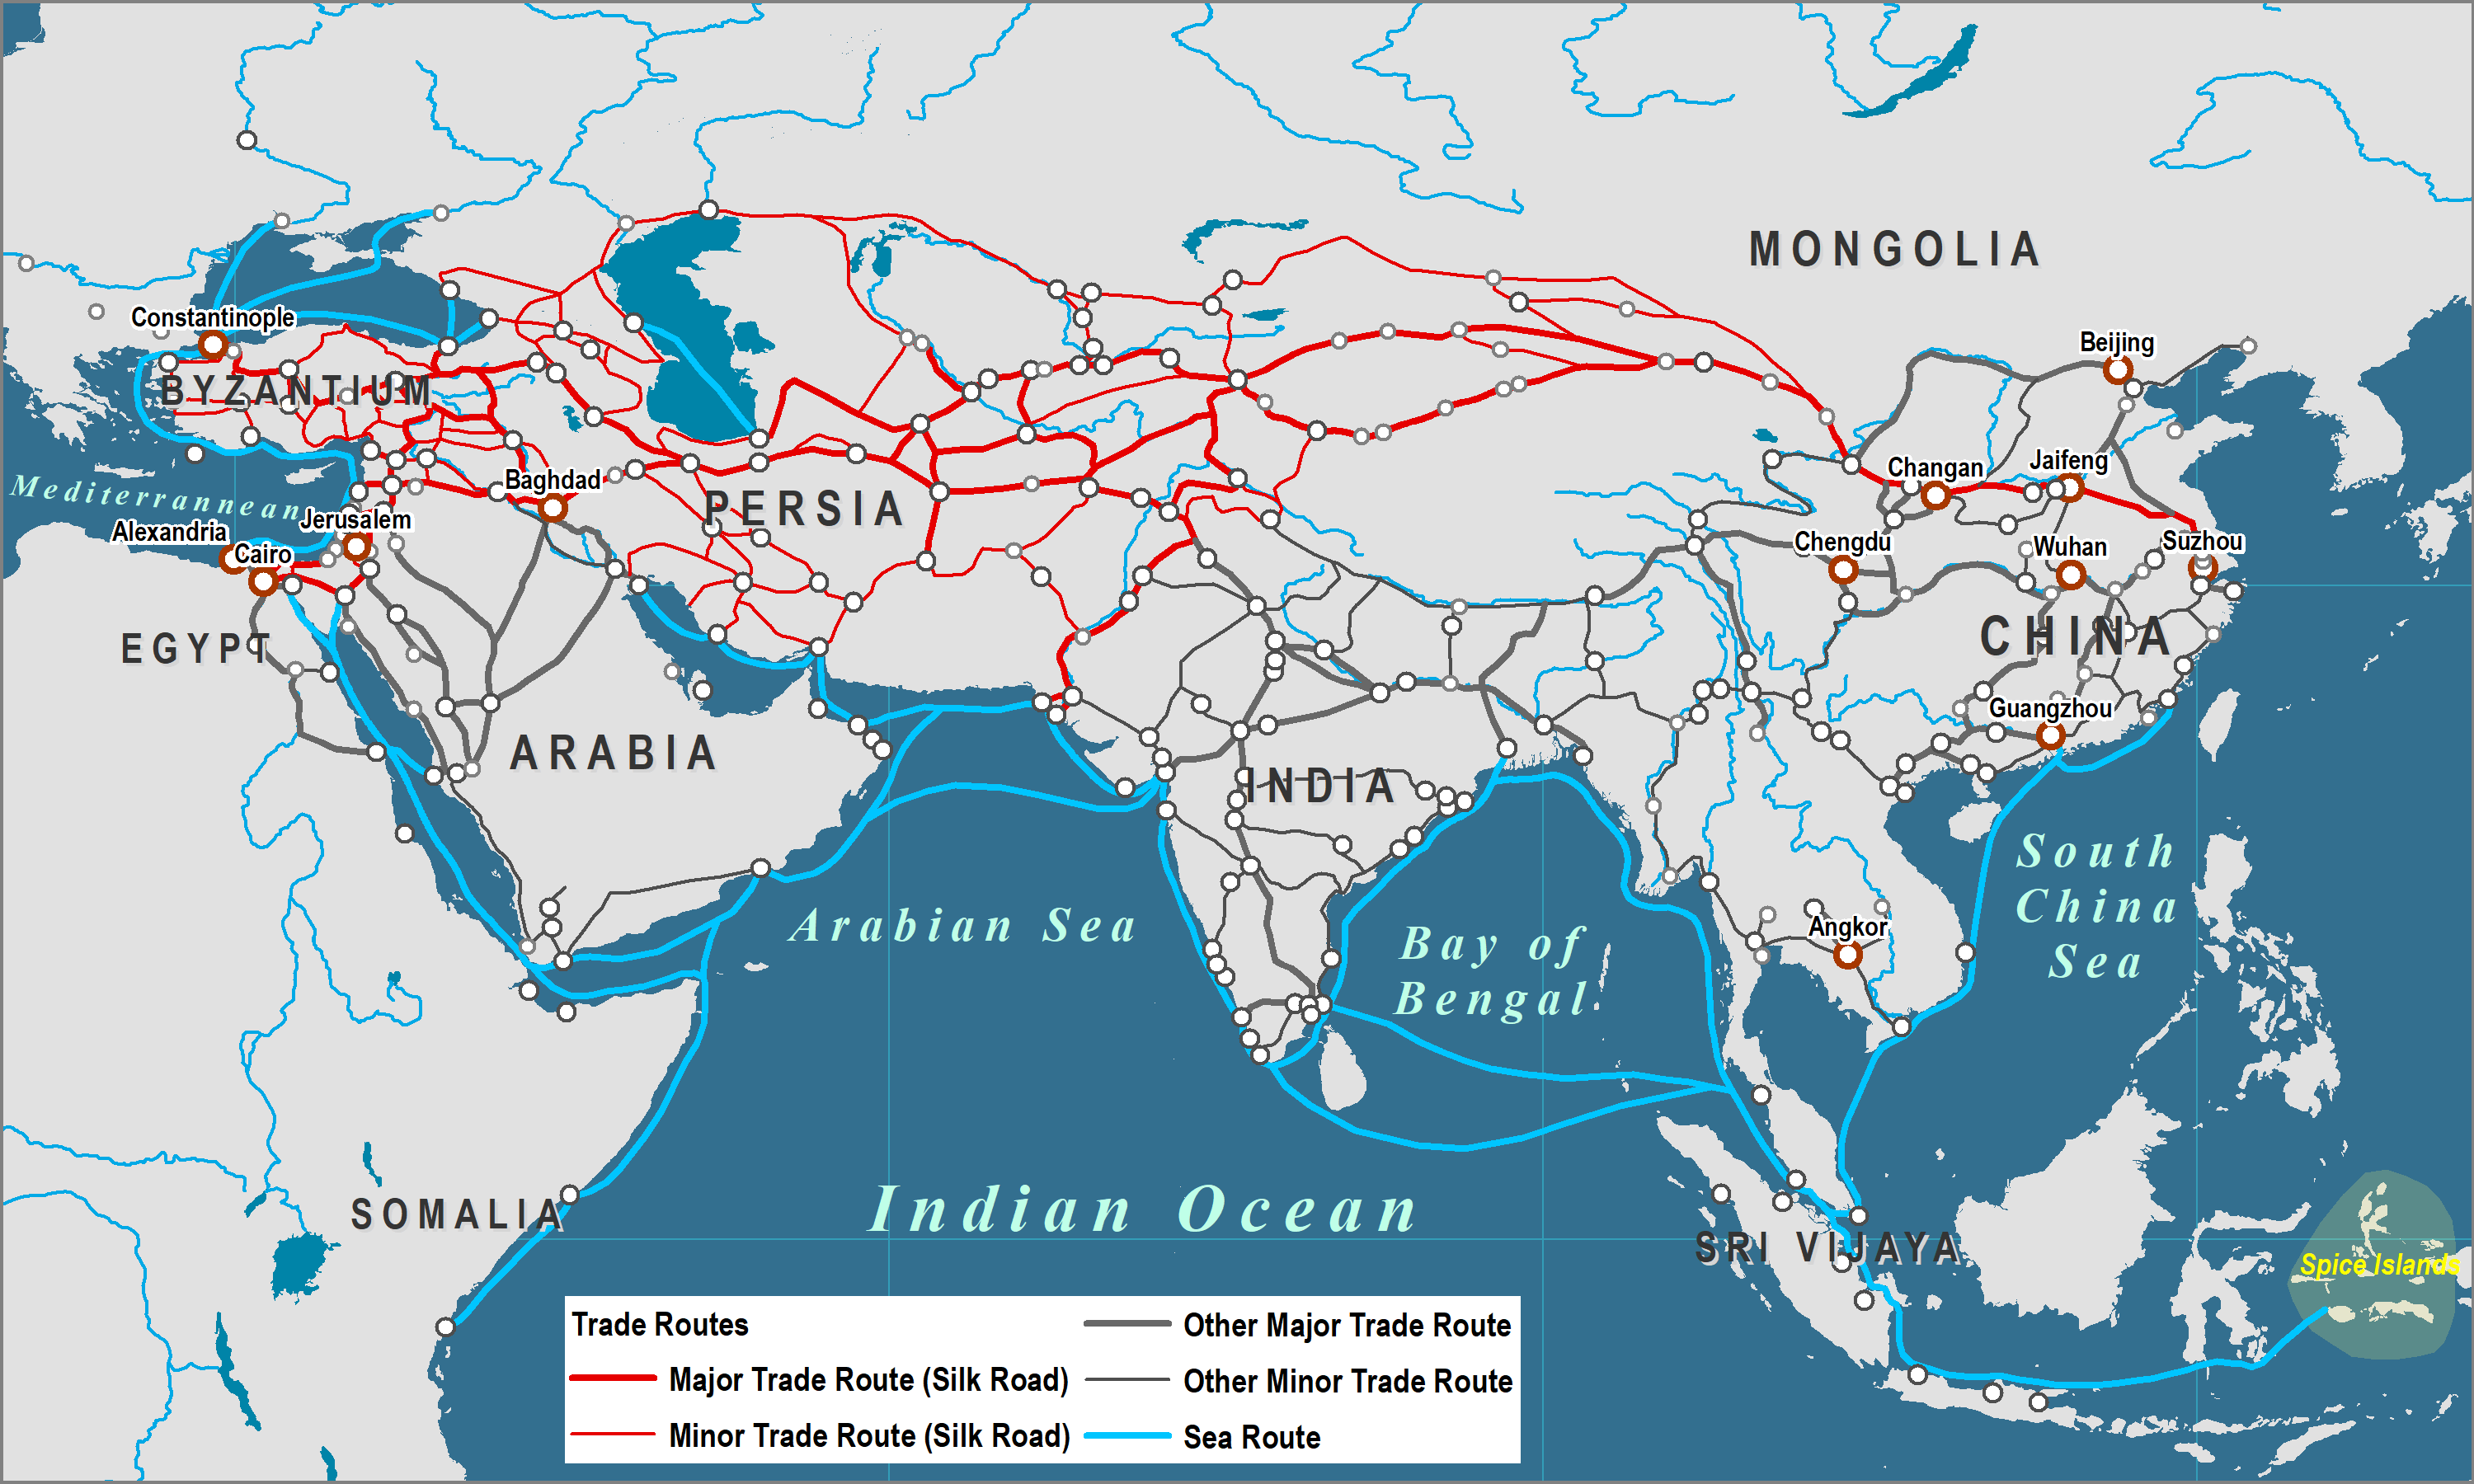
\includegraphics[max width=0.95\textwidth,
        max height=0.46000\textheight]{{Images/silkroad}.png}
    \end{center}
    \end{column}
    \end{columns}
}
\end{frame}
\begin{frame}[t]{Round 2 --- East Asia --- \mbox{Answer 10}}
\vspace{-0.5em}
\begin{columns}[T,totalwidth=\linewidth]
\begin{column}{0.32\linewidth}
\begin{block}{Question}
What is the name of the traditional Mongolian tent pictured here?
\end{block}
\visible<2->{
    \begin{block}{Answer}
    Yurt / Ger
    \end{block}
}
\end{column}
\begin{column}{0.65\linewidth}
\begin{center}
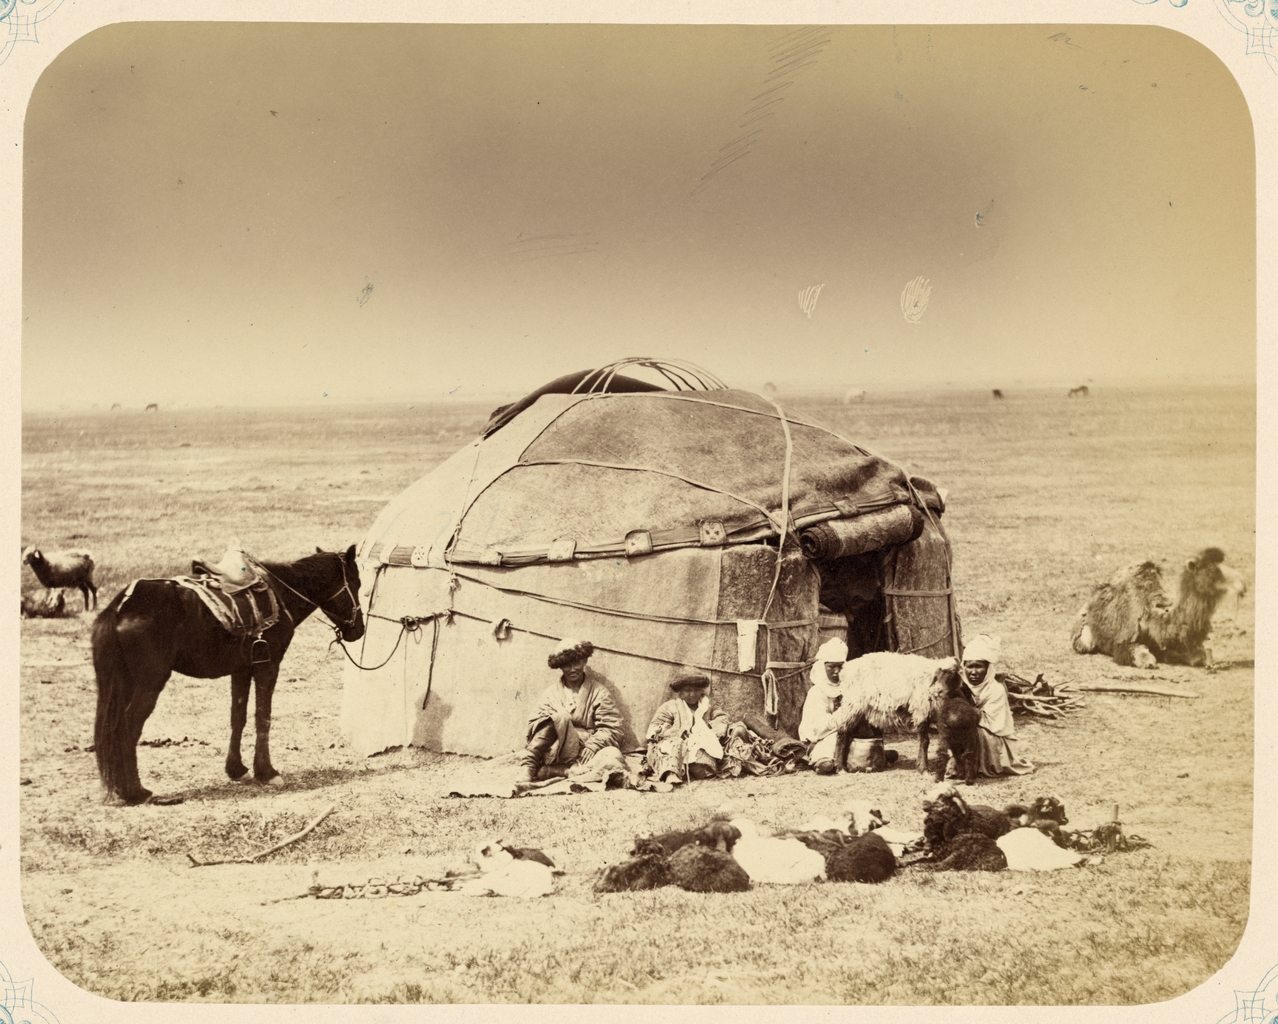
\includegraphics[max width=0.95\textwidth,max height=0.7\textheight]{{Images/yurt}.png}
\end{center}
\end{column}
\end{columns}
\end{frame}
\def\thisSectionName{Musical Instruments}
\section{Round 3}
\subsection*{Q1}
\begin{frame}[t]{Round 3 --- Musical Instruments --- \mbox{Question 1}}
\vspace{-0.5em}
\begin{block}{Question}
Which electronic instrument that is played without contact by the player is featured on the Beach Boys' ``Good Vibrations''?
\end{block}
\end{frame}
\subsection*{Q2}
\begin{frame}[t]{Round 3 --- Musical Instruments --- \mbox{Question 2}}
\vspace{-0.5em}
\begin{block}{Question}
In the Hornbostel-Sachs system of classification of musical instruments, an idiophone is an instrument that produces sound through vibration of which part of the instrument?
\end{block}
\end{frame}
\subsection*{Q3}
\begin{frame}[t]{Round 3 --- Musical Instruments --- \mbox{Question 3}}
\vspace{-0.5em}
\begin{block}{Question}
The Höfner 500/1 Violin Bass, a symmetrical model of bass guitar, was popularized by which famous left-handed bassist, who chose it because it did not look unusual when played lefty?
\end{block}
\end{frame}
\subsection*{Q4}
\begin{frame}[t]{Round 3 --- Musical Instruments --- \mbox{Question 4}}
\vspace{-0.5em}
\begin{columns}[T,totalwidth=\linewidth]
\begin{column}{0.32\linewidth}
\begin{block}{Question}
Pictured here is a drum kit with a large number of pedals on the left side and the drums mostly on the right side. Which band's kit is this? 
\end{block}
\end{column}
\begin{column}{0.65\linewidth}
\begin{center}
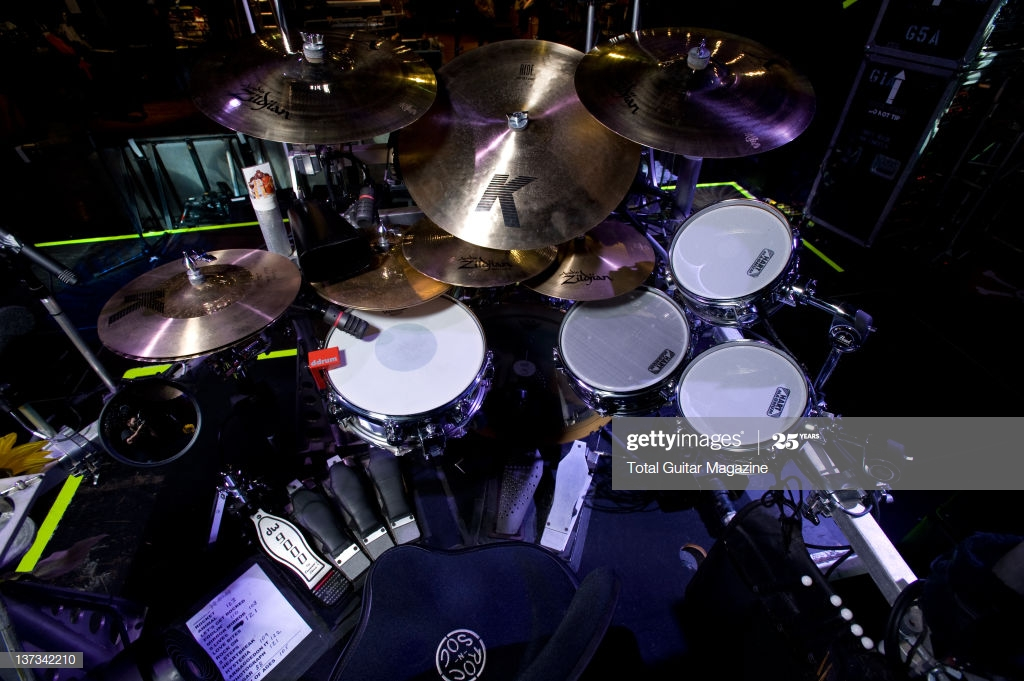
\includegraphics[max width=0.95\textwidth,max height=0.7\textheight]{{Images/defleppard}.jpg}
\end{center}
\end{column}
\end{columns}
\end{frame}
\subsection*{Q5}
\begin{frame}[t]{Round 3 --- Musical Instruments --- \mbox{Question 5}}
\vspace{-0.5em}
\begin{block}{Question}
The sackbut was a Renaissance-era version of what kind of instrument?
\end{block}
\end{frame}
\subsection*{Q6}
\begin{frame}[t]{Round 3 --- Musical Instruments --- \mbox{Question 6}}
\vspace{-0.5em}
\begin{block}{Question}
Generally speaking, which instrument do orchestras use to tune the rest of their instruments?
\end{block}
\end{frame}
\subsection*{Q7}
\begin{frame}[t]{Round 3 --- Musical Instruments --- \mbox{Question 7}}
\vspace{-0.5em}
\begin{block}{Question}
From the wood of which plant are clarinet and saxophone reeds traditionally made?
\end{block}
\end{frame}
\subsection*{Q8}
\begin{frame}[t]{Round 3 --- Musical Instruments --- \mbox{Question 8}}
\vspace{-0.5em}
\begin{block}{Question}
What is the more formal name for kettledrums?
\end{block}
\end{frame}
\subsection*{Q9}
\begin{frame}[t]{Round 3 --- Musical Instruments --- \mbox{Question 9}}
\vspace{-0.5em}
\begin{columns}[T,totalwidth=\linewidth]
\begin{column}{0.32\linewidth}
\begin{block}{Question}
What aptly-named musical instrument are the people here playing?
\end{block}
\end{column}
\begin{column}{0.65\linewidth}
\begin{center}
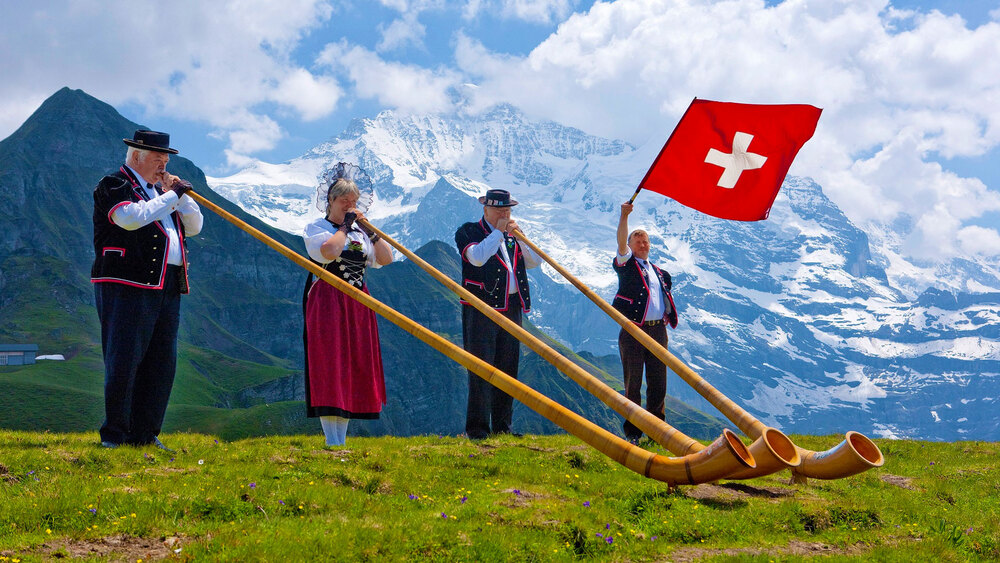
\includegraphics[max width=0.95\textwidth,max height=0.7\textheight]{{Images/alphorn}.jpg}
\end{center}
\end{column}
\end{columns}
\end{frame}
\subsection*{Q10}
\begin{frame}[t]{Round 3 --- Musical Instruments --- \mbox{Question 10}}
\vspace{-0.5em}
\begin{block}{Question}
What is the term that describes a musical instrument on which all twelve notes of the chromatic scale cannot be played?
\end{block}
\end{frame}
\subsection{Answers}
\begin{frame}[t]{Round 3 --- Musical Instruments --- \mbox{Answer 1}}
\vspace{-0.5em}
\begin{block}{Question}
Which electronic instrument that is played without contact by the player is featured on the Beach Boys' ``Good Vibrations''?
\end{block}

\visible<2->{
    \begin{columns}[T,totalwidth=\linewidth]
    \begin{column}{0.32\linewidth}
    \begin{block}{Answer}
    The theremin
    \end{block}
    \end{column}
    \begin{column}{0.65\linewidth}
    \begin{center}
    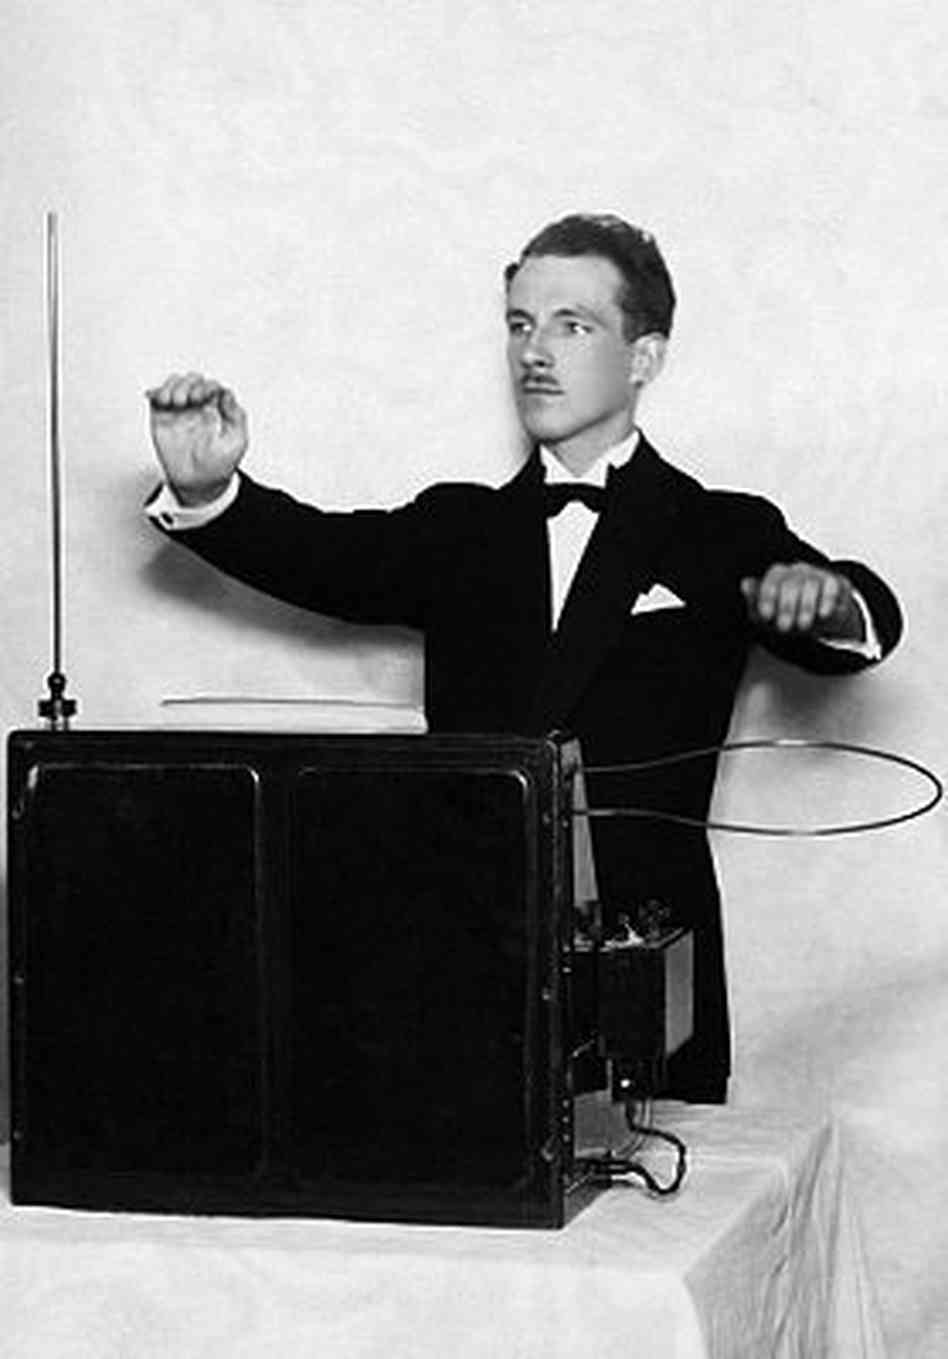
\includegraphics[max width=0.95\textwidth,
        max height=0.50000\textheight]{{Images/theramin}.jpg}
    \end{center}
    \end{column}
    \end{columns}
}
\end{frame}
\begin{frame}[t]{Round 3 --- Musical Instruments --- \mbox{Answer 2}}
\vspace{-0.5em}
\begin{block}{Question}
In the Hornbostel-Sachs system of classification of musical instruments, an idiophone is an instrument that produces sound through vibration of which part of the instrument?
\end{block}

\visible<2->{
    \begin{columns}[T,totalwidth=\linewidth]
    \begin{column}{0.32\linewidth}
    \begin{block}{Answer}
    The instrument's body / frame (e.g., a bell)
    \end{block}
    \end{column}
    \begin{column}{0.65\linewidth}
    \begin{center}
    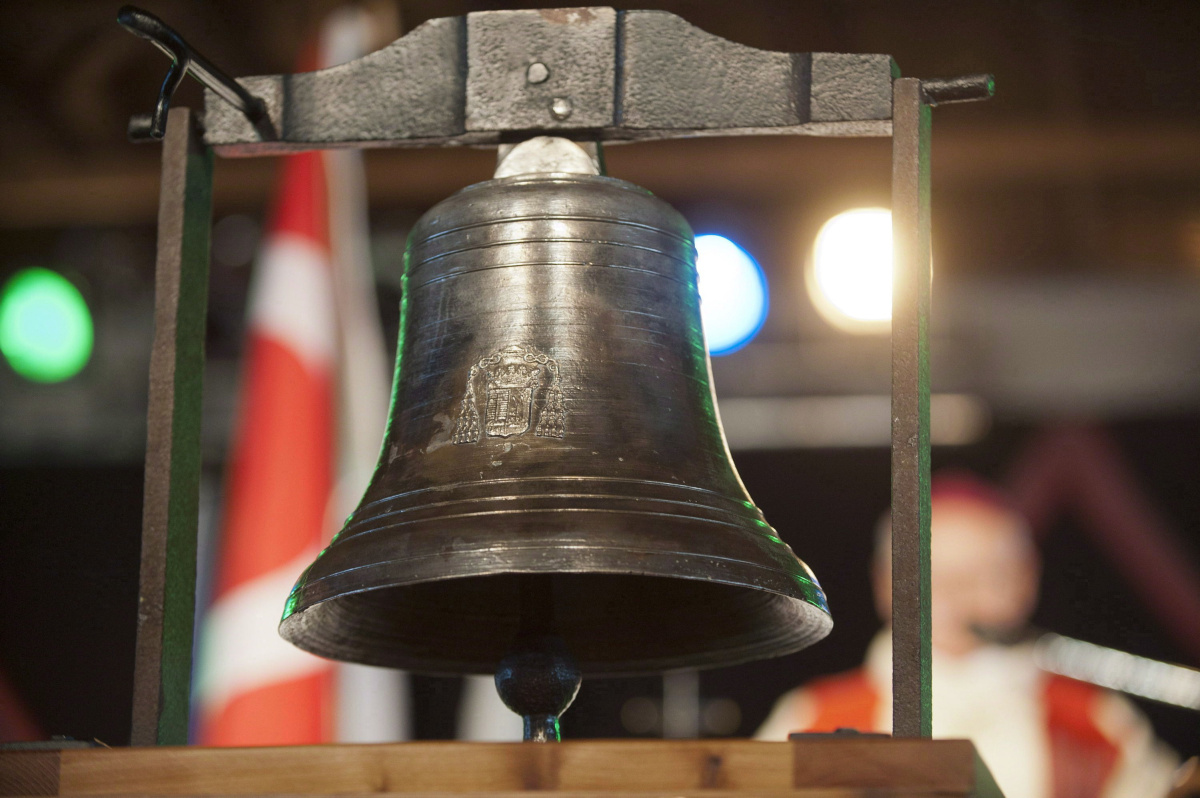
\includegraphics[max width=0.95\textwidth,
        max height=0.46000\textheight]{{Images/bell}.jpg}
    \end{center}
    \end{column}
    \end{columns}
}
\end{frame}
\begin{frame}[t]{Round 3 --- Musical Instruments --- \mbox{Answer 3}}
\vspace{-0.5em}
\begin{block}{Question}
The Höfner 500/1 Violin Bass, a symmetrical model of bass guitar, was popularized by which famous left-handed bassist, who chose it because it did not look unusual when played lefty?
\end{block}

\visible<2->{
    \begin{columns}[T,totalwidth=\linewidth]
    \begin{column}{0.32\linewidth}
    \begin{block}{Answer}
    Paul McCartney
    \end{block}
    \end{column}
    \begin{column}{0.65\linewidth}
    \begin{center}
    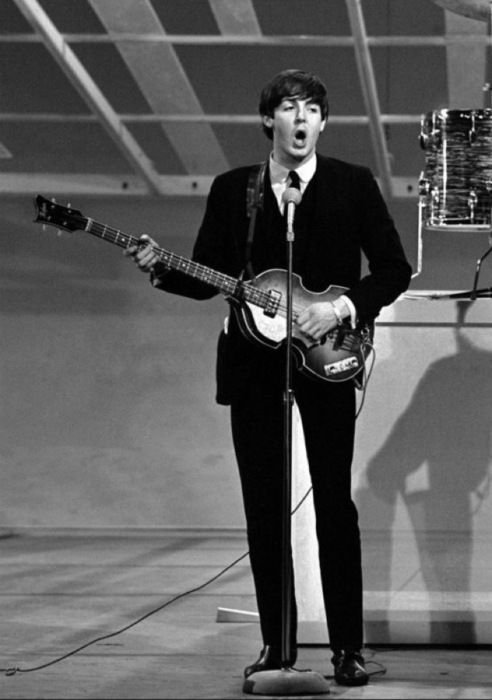
\includegraphics[max width=0.95\textwidth,
        max height=0.46000\textheight]{{Images/hofner}.jpg}
    \end{center}
    \end{column}
    \end{columns}
}
\end{frame}
\begin{frame}[t]{Round 3 --- Musical Instruments --- \mbox{Answer 4}}
\vspace{-0.5em}
\begin{columns}[T,totalwidth=\linewidth]
\begin{column}{0.38\linewidth}
\begin{block}{Question}
Pictured here is a drum kit with a large number of pedals on the left side and the drums mostly on the right side. Which band's kit is this? 
\end{block}
\end{column}
\begin{column}{0.6\linewidth}
\begin{center}
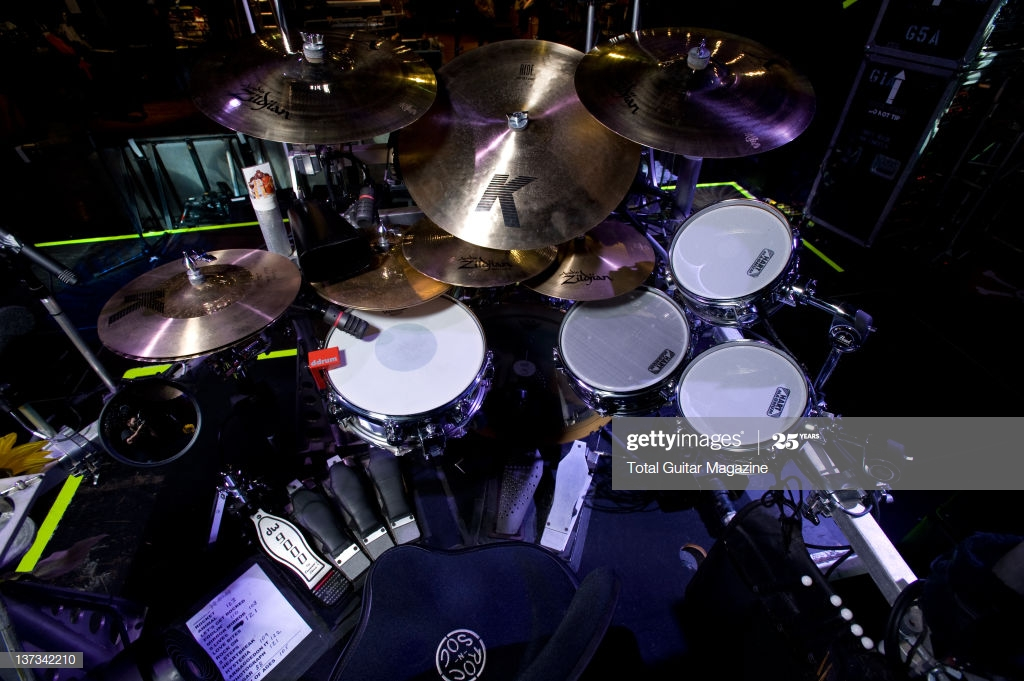
\includegraphics[max width=0.95\textwidth,max height=0.35\textheight]{{Images/defleppard}.jpg}
\end{center}
\end{column}
\end{columns}

\visible<2->{
    \begin{columns}[T,totalwidth=\linewidth]
    \begin{column}{0.38\linewidth}
    \begin{block}{Answer}
    Def Leppard (whose drummer lost his left arm yet continued to play for them)
    \end{block}
    \end{column}
    \begin{column}{0.6\linewidth}
    \begin{center}
    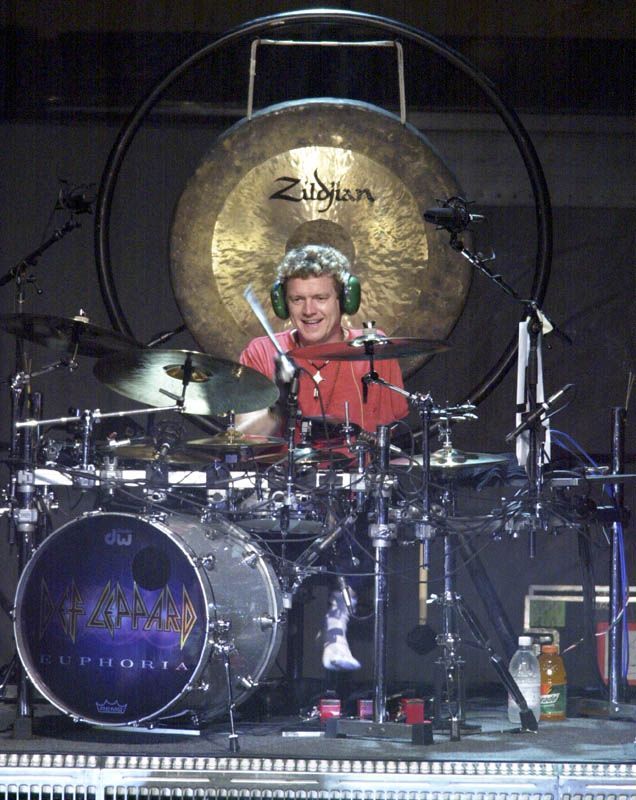
\includegraphics[max width=0.95\textwidth,
        max height=0.34\textheight]{{Images/deflepp}.jpg}
    \end{center}
    \end{column}
    \end{columns}
}
\end{frame}
\begin{frame}[t]{Round 3 --- Musical Instruments --- \mbox{Answer 5}}
\vspace{-0.5em}
\begin{block}{Question}
The sackbut was a Renaissance-era version of what kind of instrument?
\end{block}

\visible<2->{
    \begin{columns}[T,totalwidth=\linewidth]
    \begin{column}{0.32\linewidth}
    \begin{block}{Answer}
    The trombone
    \end{block}
    \end{column}
    \begin{column}{0.65\linewidth}
    \begin{center}
    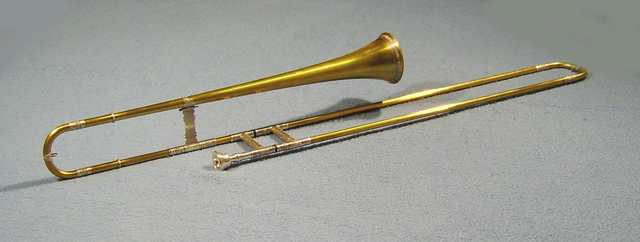
\includegraphics[max width=0.95\textwidth,
        max height=0.54000\textheight]{{Images/sackbut}.jpg}
    \end{center}
    \end{column}
    \end{columns}
}
\end{frame}
\begin{frame}[t]{Round 3 --- Musical Instruments --- \mbox{Answer 6}}
\vspace{-0.5em}
\begin{block}{Question}
Generally speaking, which instrument do orchestras use to tune the rest of their instruments?
\end{block}

\visible<2->{
    \begin{columns}[T,totalwidth=\linewidth]
    \begin{column}{0.32\linewidth}
    \begin{block}{Answer}
    The oboe
    \end{block}
    \end{column}
    \begin{column}{0.65\linewidth}
    \begin{center}
    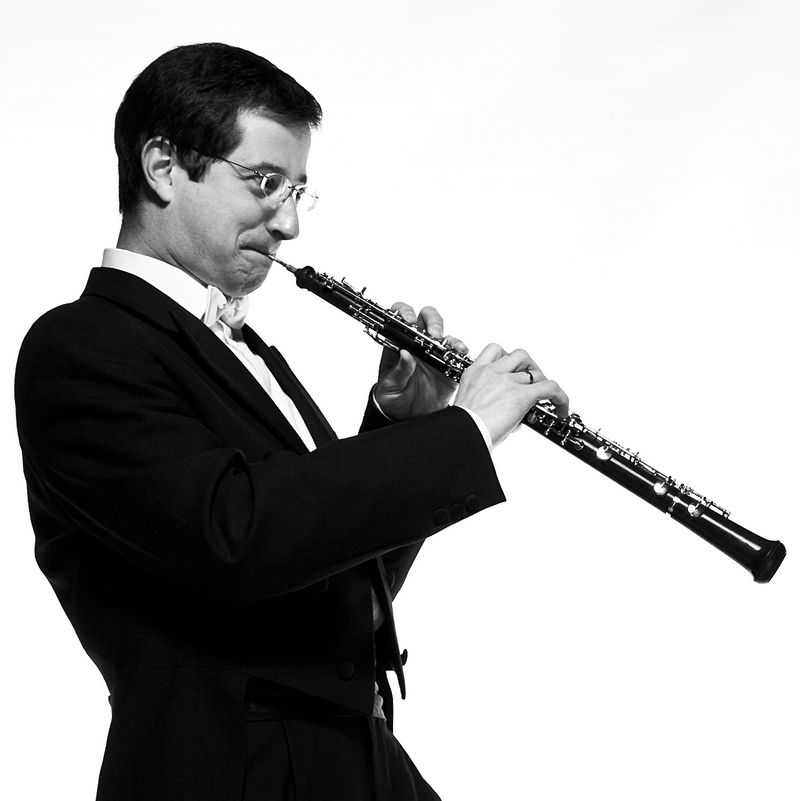
\includegraphics[max width=0.95\textwidth,
        max height=0.54000\textheight]{{Images/oboe}.jpg}
    \end{center}
    \end{column}
    \end{columns}
}
\end{frame}
\begin{frame}[t]{Round 3 --- Musical Instruments --- \mbox{Answer 7}}
\vspace{-0.5em}
\begin{block}{Question}
From the wood of which plant are clarinet and saxophone reeds traditionally made?
\end{block}

\visible<2->{
    \begin{columns}[T,totalwidth=\linewidth]
    \begin{column}{0.32\linewidth}
    \begin{block}{Answer}
    Giant cane / cane / giant reed / elephant grass / Spanish cane / \emph{Arundo donax}
    \end{block}
    \end{column}
    \begin{column}{0.65\linewidth}
    \begin{center}
    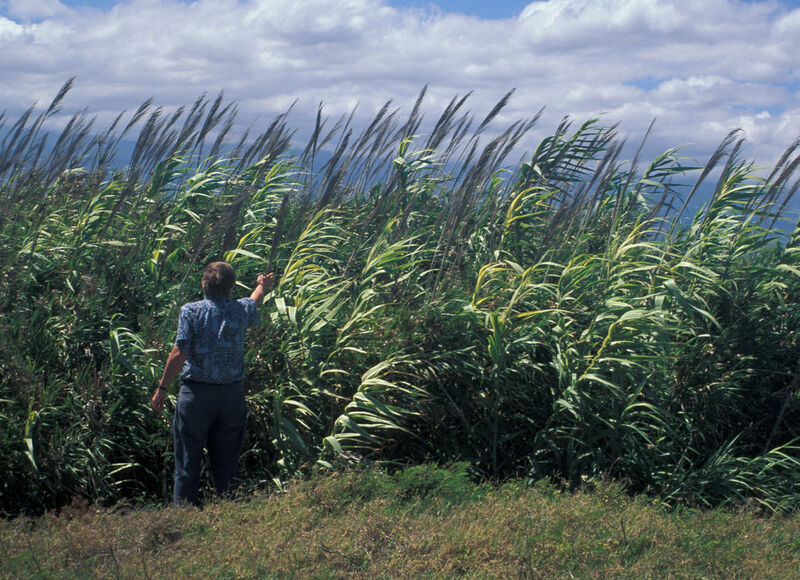
\includegraphics[max width=0.95\textwidth,
        max height=0.54000\textheight]{{Images/reed}.jpg}
    \end{center}
    \end{column}
    \end{columns}
}
\end{frame}
\begin{frame}[t]{Round 3 --- Musical Instruments --- \mbox{Answer 8}}
\vspace{-0.5em}
\begin{block}{Question}
What is the more formal name for kettledrums?
\end{block}

\visible<2->{
    \begin{columns}[T,totalwidth=\linewidth]
    \begin{column}{0.32\linewidth}
    \begin{block}{Answer}
    Timpani
    \end{block}
    \end{column}
    \begin{column}{0.65\linewidth}
    \begin{center}
    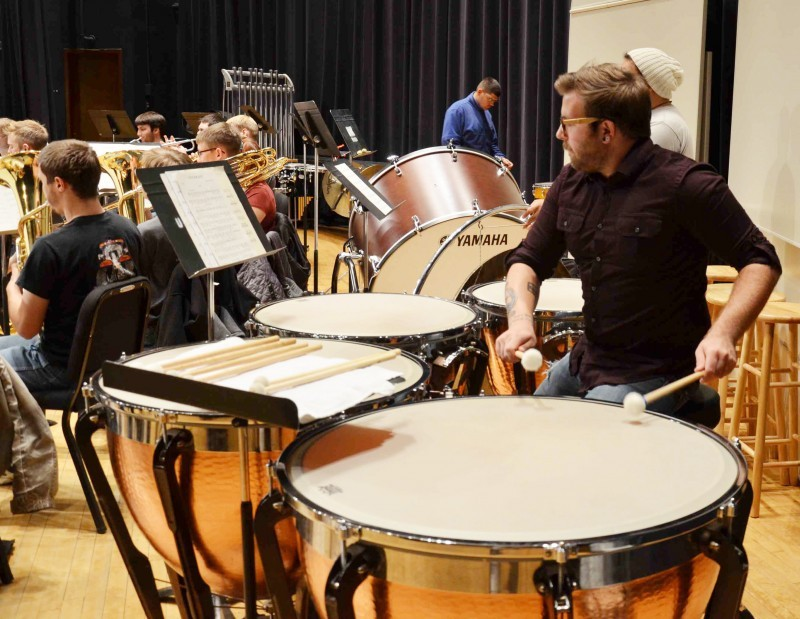
\includegraphics[max width=0.95\textwidth,
        max height=0.58000\textheight]{{Images/timpani}.jpg}
    \end{center}
    \end{column}
    \end{columns}
}
\end{frame}
\begin{frame}[t]{Round 3 --- Musical Instruments --- \mbox{Answer 9}}
\vspace{-0.5em}
\begin{columns}[T,totalwidth=\linewidth]
\begin{column}{0.32\linewidth}
\begin{block}{Question}
What aptly-named musical instrument are the people here playing?
\end{block}
\visible<2->{
    \begin{block}{Answer}
    The alphorn / alpenhorn / alpine horn
    \end{block}
}
\end{column}
\begin{column}{0.65\linewidth}
\begin{center}
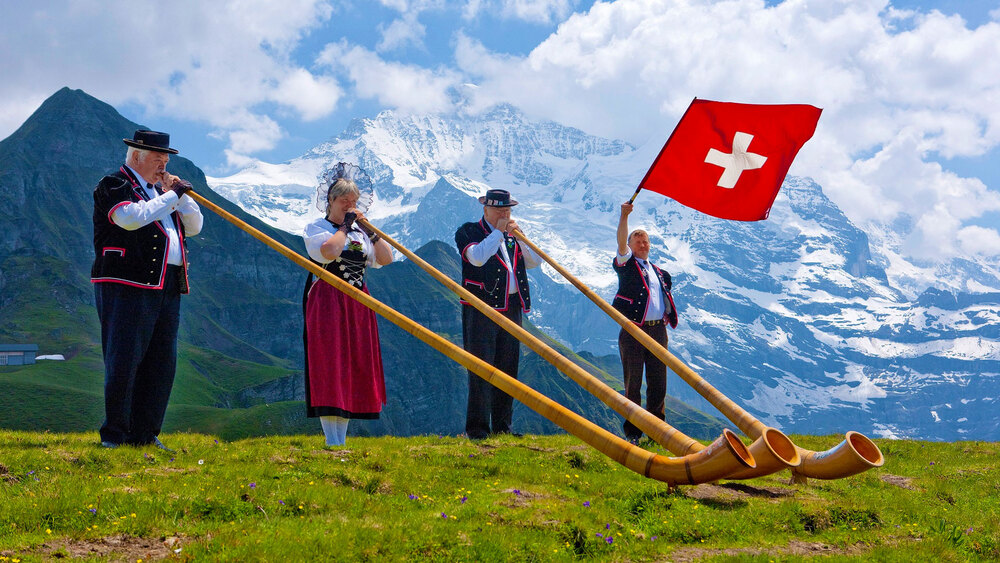
\includegraphics[max width=0.95\textwidth,max height=0.7\textheight]{{Images/alphorn}.jpg}
\end{center}
\end{column}
\end{columns}
\end{frame}
\begin{frame}[t]{Round 3 --- Musical Instruments --- \mbox{Answer 10}}
\vspace{-0.5em}
\begin{block}{Question}
What is the term that describes a musical instrument on which all twelve notes of the chromatic scale cannot be played?
\end{block}

\visible<2->{
    \begin{columns}[T,totalwidth=\linewidth]
    \begin{column}{0.32\linewidth}
    \begin{block}{Answer}
    Diatonic
    \end{block}
    \end{column}
    \begin{column}{0.65\linewidth}
    \begin{center}
    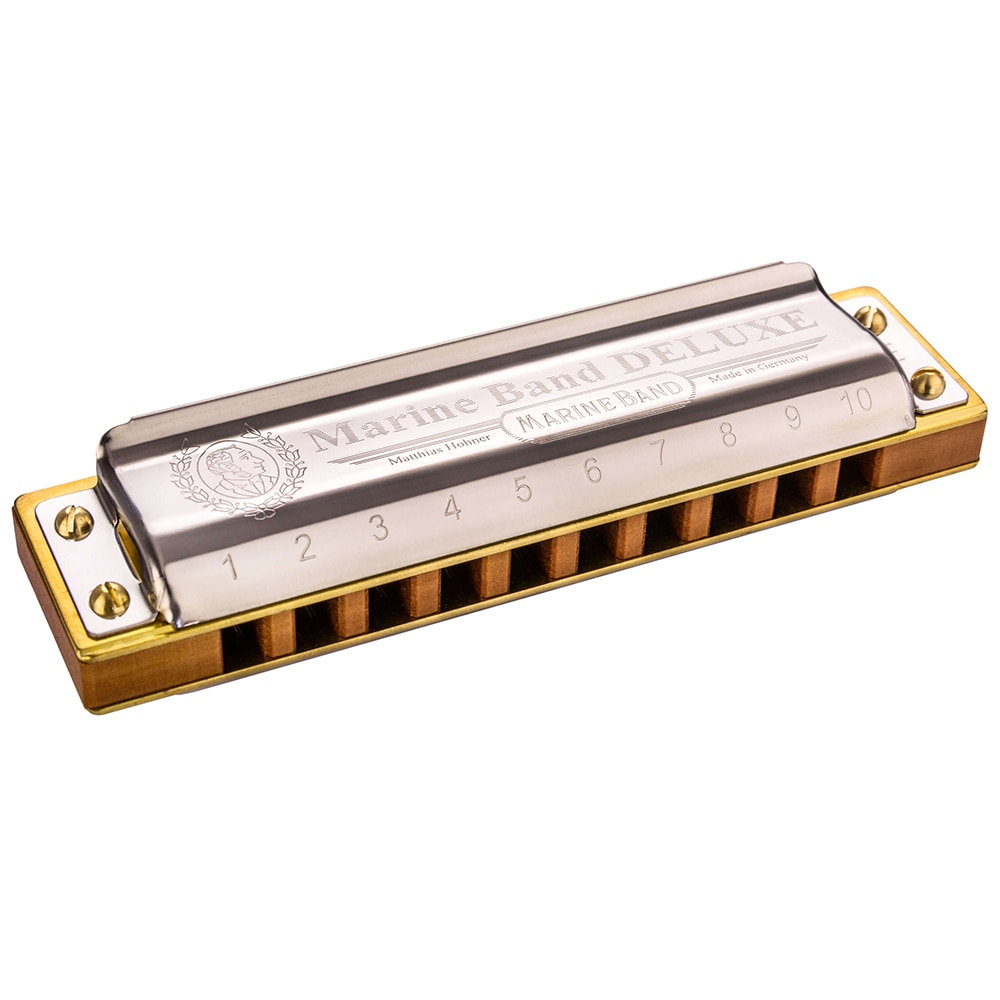
\includegraphics[max width=0.95\textwidth,
        max height=0.50000\textheight]{{Images/harmonica}.jpg}
    \end{center}
    \end{column}
    \end{columns}
}
\end{frame}
\def\thisSectionName{Outer Space}
\section{Round 4}
\subsection*{Q1}
\begin{frame}[t]{Round 4 --- Outer Space --- \mbox{Question 1}}
\vspace{-0.5em}
\begin{block}{Question}
To within a billion years, how old is the universe?
\end{block}
\end{frame}
\subsection*{Q2}
\begin{frame}[t]{Round 4 --- Outer Space --- \mbox{Question 2}}
\vspace{-0.5em}
\begin{block}{Question}
When a planet revolves around a star, approximately what shape does its orbit trace?
\end{block}
\end{frame}
\subsection*{Q3}
\begin{frame}[t]{Round 4 --- Outer Space --- \mbox{Question 3}}
\vspace{-0.5em}
\begin{block}{Question}
Which star is the brightest star in the night sky?
\end{block}
\end{frame}
\subsection*{Q4}
\begin{frame}[t]{Round 4 --- Outer Space --- \mbox{Question 4}}
\vspace{-0.5em}
\begin{block}{Question}
In 5 to 6 billion years, the Sun will have died and will spend the rest of its existence as what kind of star?
\end{block}
\end{frame}
\subsection*{Q5}
\begin{frame}[t]{Round 4 --- Outer Space --- \mbox{Question 5}}
\vspace{-0.5em}
\begin{columns}[T,totalwidth=\linewidth]
\begin{column}{0.32\linewidth}
\begin{block}{Question}
What is this a photograph of?
\end{block}
\end{column}
\begin{column}{0.65\linewidth}
\begin{center}
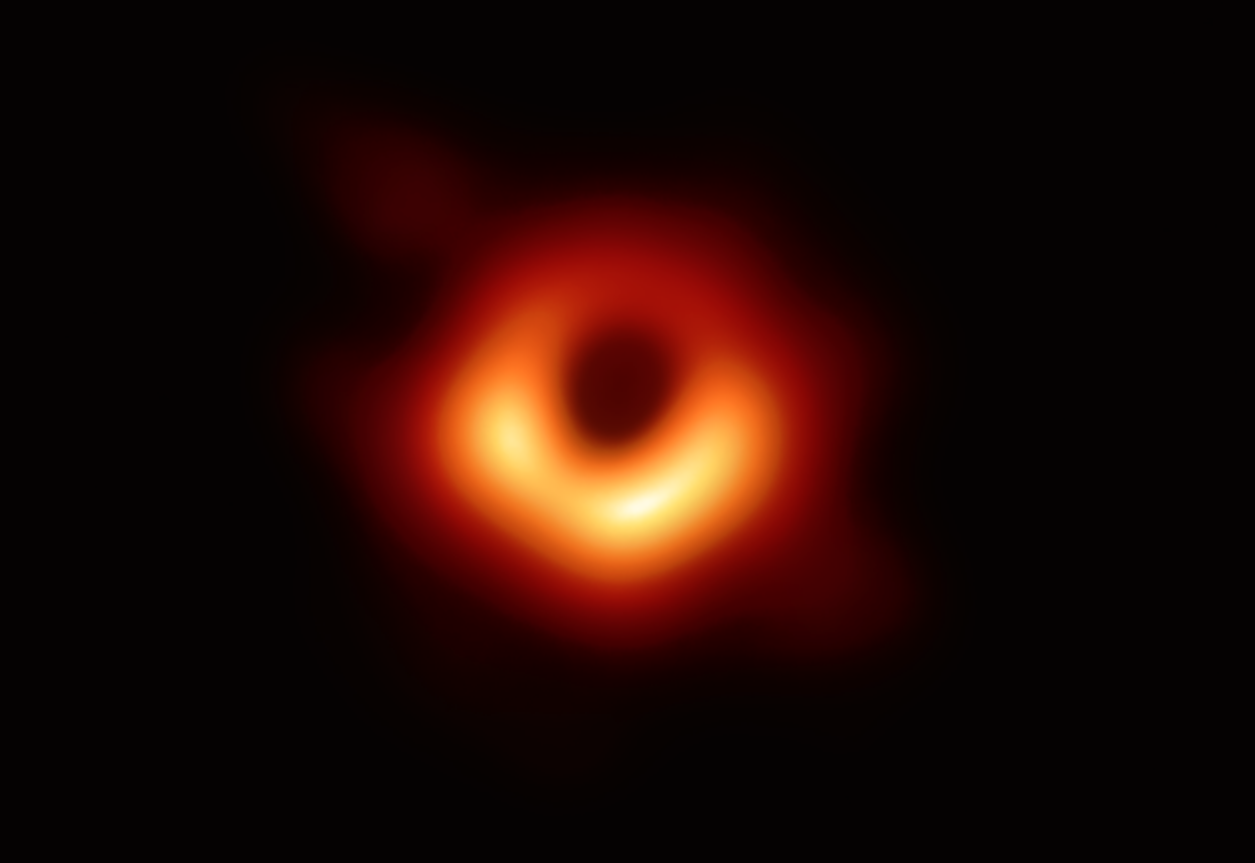
\includegraphics[max width=0.95\textwidth,max height=0.7\textheight]{{Images/blackhole}.png}
\end{center}
\end{column}
\end{columns}
\end{frame}
\subsection*{Q6}
\begin{frame}[t]{Round 4 --- Outer Space --- \mbox{Question 6}}
\vspace{-0.5em}
\begin{block}{Question}
The precession, or rotation of orbit, of which planet lent some of the earliest support to Einstein's theory of general relativity?
\end{block}
\end{frame}
\subsection*{Q7}
\begin{frame}[t]{Round 4 --- Outer Space --- \mbox{Question 7}}
\vspace{-0.5em}
\begin{block}{Question}
Which man-made object is currently farthest from Earth?
\end{block}
\end{frame}
\subsection*{Q8}
\begin{frame}[t]{Round 4 --- Outer Space --- \mbox{Question 8}}
\vspace{-0.5em}
\begin{block}{Question}
First observed in 1610, the moons of which planet were the first extraterrestrial objects discovered that were not principally orbiting the Earth or the Sun?
\end{block}
\end{frame}
\subsection*{Q9}
\begin{frame}[t]{Round 4 --- Outer Space --- \mbox{Question 9}}
\vspace{-0.5em}
\begin{block}{Question}
Which star outside our solar system is the closest star to our solar system?
\end{block}
\end{frame}
\subsection*{Q10}
\begin{frame}[t]{Round 4 --- Outer Space --- \mbox{Question 10}}
\vspace{-0.5em}
\begin{block}{Question}
Who currently holds the record for the most cumulative time spent in outer space?
\end{block}
\end{frame}
\subsection{Answers}
\begin{frame}[t]{Round 4 --- Outer Space --- \mbox{Answer 1}}
\vspace{-0.5em}
\begin{block}{Question}
To within a billion years, how old is the universe?
\end{block}

\visible<2->{
    \begin{columns}[T,totalwidth=\linewidth]
    \begin{column}{0.32\linewidth}
    \begin{block}{Answer}
    13.8 billion years (12.8B-14.8B will be accepted)
    \end{block}
    \end{column}
    \begin{column}{0.65\linewidth}
    \begin{center}
    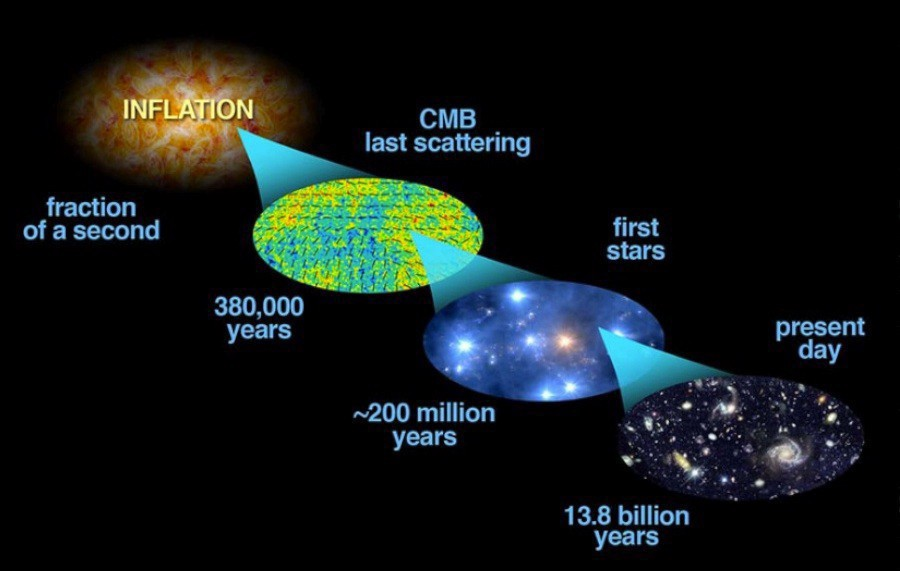
\includegraphics[max width=0.95\textwidth,
        max height=0.54000\textheight]{{Images/universeage}.jpeg}
    \end{center}
    \end{column}
    \end{columns}
}
\end{frame}
\begin{frame}[t]{Round 4 --- Outer Space --- \mbox{Answer 2}}
\vspace{-0.5em}
\begin{block}{Question}
When a planet revolves around a star, approximately what shape does its orbit trace?
\end{block}

\visible<2->{
    \begin{columns}[T,totalwidth=\linewidth]
    \begin{column}{0.32\linewidth}
    \begin{block}{Answer}
    An ellipse
    \end{block}
    \end{column}
    \begin{column}{0.65\linewidth}
    \begin{center}
    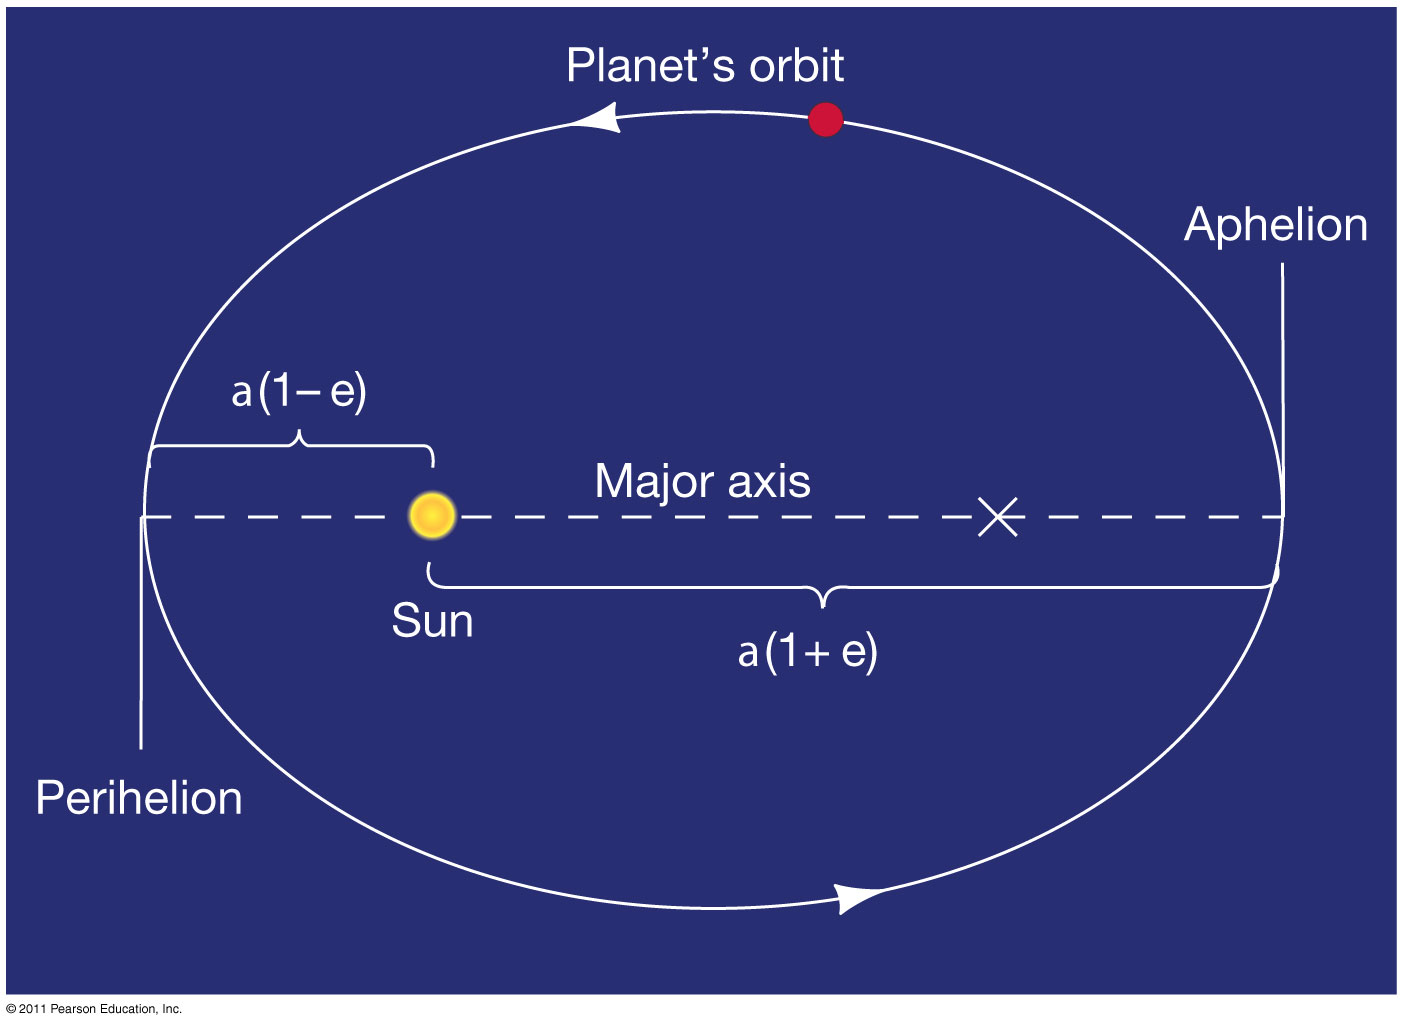
\includegraphics[max width=0.95\textwidth,
        max height=0.54000\textheight]{{Images/ellipse}.jpg}
    \end{center}
    \end{column}
    \end{columns}
}
\end{frame}
\begin{frame}[t]{Round 4 --- Outer Space --- \mbox{Answer 3}}
\vspace{-0.5em}
\begin{block}{Question}
Which star is the brightest star in the night sky?
\end{block}

\visible<2->{
    \begin{columns}[T,totalwidth=\linewidth]
    \begin{column}{0.32\linewidth}
    \begin{block}{Answer}
    Sirius
    \end{block}
    \end{column}
    \begin{column}{0.65\linewidth}
    \begin{center}
    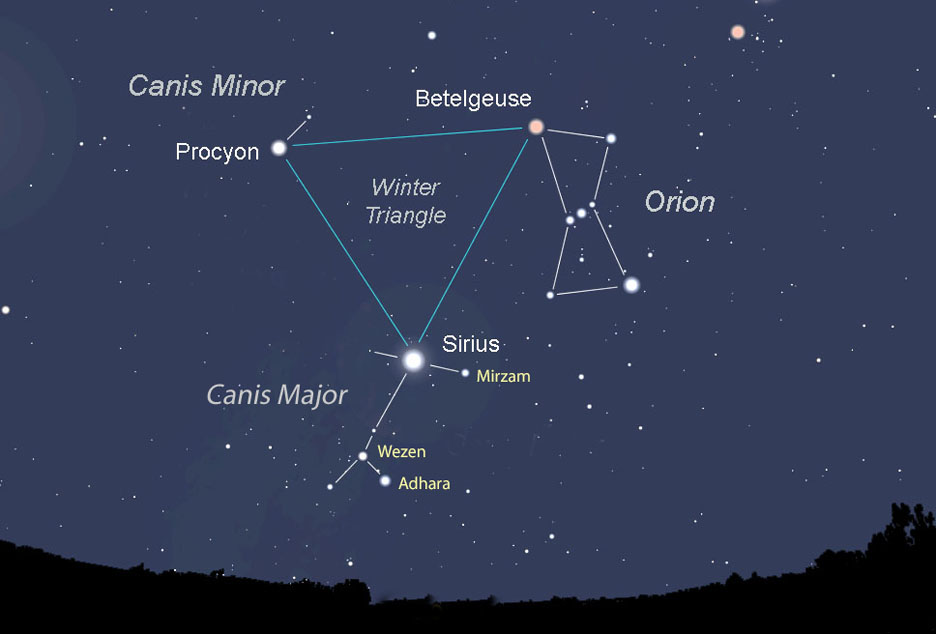
\includegraphics[max width=0.95\textwidth,
        max height=0.58000\textheight]{{Images/sirius}.jpg}
    \end{center}
    \end{column}
    \end{columns}
}
\end{frame}
\begin{frame}[t]{Round 4 --- Outer Space --- \mbox{Answer 4}}
\vspace{-0.5em}
\begin{block}{Question}
In 5 to 6 billion years, the Sun will have died and will spend the rest of its existence as what kind of star?
\end{block}

\visible<2->{
    \begin{columns}[T,totalwidth=\linewidth]
    \begin{column}{0.32\linewidth}
    \begin{block}{Answer}
    A white dwarf
    \end{block}
    \end{column}
    \begin{column}{0.65\linewidth}
    \begin{center}
    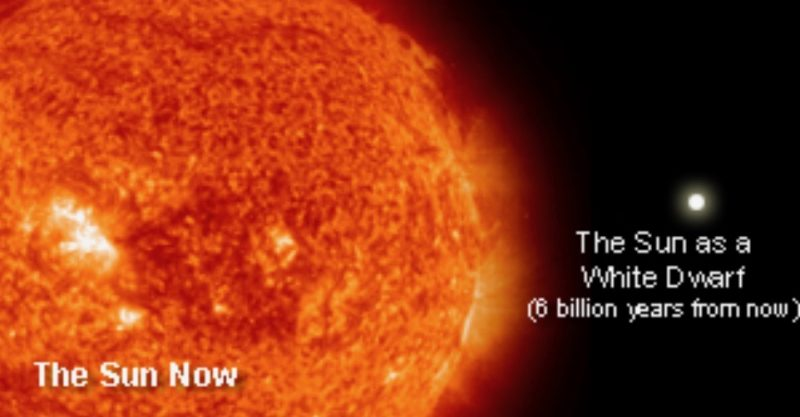
\includegraphics[max width=0.95\textwidth,
        max height=0.50000\textheight]{{Images/whitedwarf}.jpg}
    \end{center}
    \end{column}
    \end{columns}
}
\end{frame}
\begin{frame}[t]{Round 4 --- Outer Space --- \mbox{Answer 5}}
\vspace{-0.5em}
\begin{columns}[T,totalwidth=\linewidth]
\begin{column}{0.32\linewidth}
\begin{block}{Question}
What is this a photograph of?
\end{block}
\visible<2->{
    \begin{block}{Answer}
    A black hole
    \end{block}
}
\end{column}
\begin{column}{0.65\linewidth}
\begin{center}
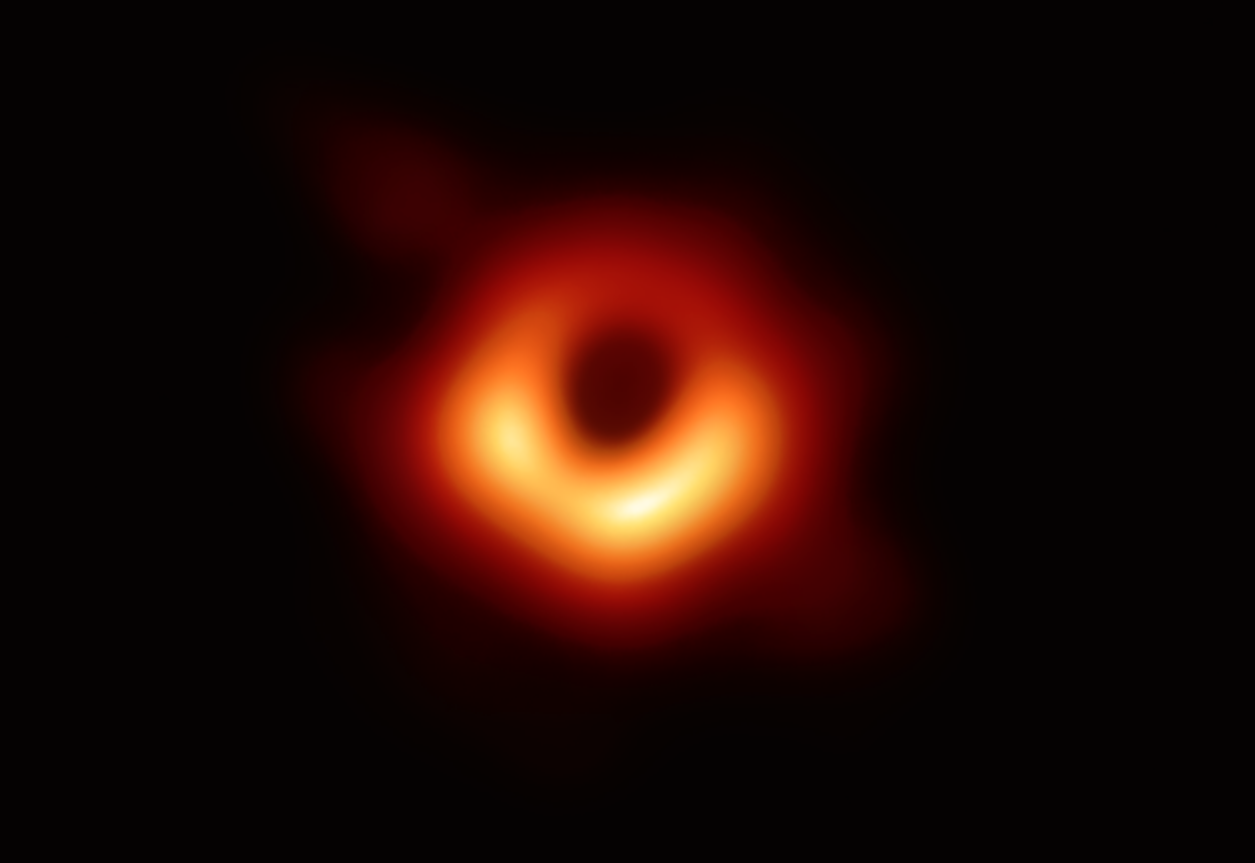
\includegraphics[max width=0.95\textwidth,max height=0.7\textheight]{{Images/blackhole}.png}
\end{center}
\end{column}
\end{columns}
\end{frame}
\begin{frame}[t]{Round 4 --- Outer Space --- \mbox{Answer 6}}
\vspace{-0.5em}
\begin{block}{Question}
The precession, or rotation of orbit, of which planet lent some of the earliest support to Einstein's theory of general relativity?
\end{block}

\visible<2->{
    \begin{columns}[T,totalwidth=\linewidth]
    \begin{column}{0.32\linewidth}
    \begin{block}{Answer}
    Mercury
    \end{block}
    \end{column}
    \begin{column}{0.65\linewidth}
    \begin{center}
    \includegraphics[max width=0.95\textwidth,
        max height=0.50000\textheight]{{Images/precession}.png}
    \end{center}
    \end{column}
    \end{columns}
}
\end{frame}
\begin{frame}[t]{Round 4 --- Outer Space --- \mbox{Answer 7}}
\vspace{-0.5em}
\begin{block}{Question}
Which man-made object is currently farthest from Earth?
\end{block}

\visible<2->{
    \begin{columns}[T,totalwidth=\linewidth]
    \begin{column}{0.32\linewidth}
    \begin{block}{Answer}
    Voyager 1
    \end{block}
    \end{column}
    \begin{column}{0.65\linewidth}
    \begin{center}
    \includegraphics[max width=0.95\textwidth,
        max height=0.54000\textheight]{{Images/voyager1}.jpeg}
    \end{center}
    \end{column}
    \end{columns}
}
\end{frame}
\begin{frame}[t]{Round 4 --- Outer Space --- \mbox{Answer 8}}
\vspace{-0.5em}
\begin{block}{Question}
First observed in 1610, the moons of which planet were the first extraterrestrial objects discovered that were not principally orbiting the Earth or the Sun?
\end{block}

\visible<2->{
    \begin{columns}[T,totalwidth=\linewidth]
    \begin{column}{0.32\linewidth}
    \begin{block}{Answer}
    Jupiter
    \end{block}
    \end{column}
    \begin{column}{0.65\linewidth}
    \begin{center}
    \includegraphics[max width=0.95\textwidth,
        max height=0.46000\textheight]{{Images/jupitermoons}.jpg}
    \end{center}
    \end{column}
    \end{columns}
}
\end{frame}
\begin{frame}[t]{Round 4 --- Outer Space --- \mbox{Answer 9}}
\vspace{-0.5em}
\begin{block}{Question}
Which star outside our solar system is the closest star to our solar system?
\end{block}

\visible<2->{
    \begin{columns}[T,totalwidth=\linewidth]
    \begin{column}{0.32\linewidth}
    \begin{block}{Answer}
    Proxima Centauri
    \end{block}
    \end{column}
    \begin{column}{0.65\linewidth}
    \begin{center}
    \includegraphics[max width=0.95\textwidth,
        max height=0.54000\textheight]{{Images/centauri}.jpg}
    \end{center}
    \end{column}
    \end{columns}
}
\end{frame}
\begin{frame}[t]{Round 4 --- Outer Space --- \mbox{Answer 10}}
\vspace{-0.5em}
\begin{block}{Question}
Who currently holds the record for the most cumulative time spent in outer space?
\end{block}

\visible<2->{
    \begin{columns}[T,totalwidth=\linewidth]
    \begin{column}{0.32\linewidth}
    \begin{block}{Answer}
    Gennady Padalka
    \end{block}
    \end{column}
    \begin{column}{0.65\linewidth}
    \begin{center}
    \includegraphics[max width=0.95\textwidth,
        max height=0.54000\textheight]{{Images/padalka}.jpg}
    \end{center}
    \end{column}
    \end{columns}
}
\end{frame}
\def\thisSectionName{Saturday Night Live}
\section{Round 5}
\subsection*{Q1}
\begin{frame}[t]{Round 5 --- Saturday Night Live --- \mbox{Question 1}}
\vspace{-0.5em}
\begin{block}{Question}
What name did the SNL ensemble originally go by?
\end{block}
\end{frame}
\subsection*{Q2}
\begin{frame}[t]{Round 5 --- Saturday Night Live --- \mbox{Question 2}}
\vspace{-0.5em}
\begin{block}{Question}
Who hosted the very first episode of SNL\@?
\end{block}
\end{frame}
\subsection*{Q3}
\begin{frame}[t]{Round 5 --- Saturday Night Live --- \mbox{Question 3}}
\vspace{-0.5em}
\begin{block}{Question}
Who was the original host of Weekend Update?
\end{block}
\end{frame}
\subsection*{Q4}
\begin{frame}[t]{Round 5 --- Saturday Night Live --- \mbox{Question 4}}
\vspace{-0.5em}
\begin{block}{Question}
Who has hosted SNL the greatest number of times?
\end{block}
\end{frame}
\subsection*{Q5}
\begin{frame}[t]{Round 5 --- Saturday Night Live --- \mbox{Question 5}}
\vspace{-0.5em}
\begin{block}{Question}
Which former child star was the first SNL cast member to be born after the show's premier in 1975?
\end{block}
\end{frame}
\subsection*{Q6}
\begin{frame}[t]{Round 5 --- Saturday Night Live --- \mbox{Question 6}}
\vspace{-0.5em}
\begin{block}{Question}
Christopher Walken's SNL character ``\emph{The} Bruce Dickinson'' had a fever, and the only prescription was what?
\end{block}
\end{frame}
\subsection*{Q7}
\begin{frame}[t]{Round 5 --- Saturday Night Live --- \mbox{Question 7}}
\vspace{-0.5em}
\begin{block}{Question}
What is the name of the motivational speaker character who lives ``in a van down by the river''?
\end{block}
\end{frame}
\subsection*{Q8}
\begin{frame}[t]{Round 5 --- Saturday Night Live --- \mbox{Question 8}}
\vspace{-0.5em}
\begin{block}{Question}
Which studio in 30 Rockefeller Plaza is SNL filmed in?
\end{block}
\end{frame}
\subsection*{Q9}
\begin{frame}[t]{Round 5 --- Saturday Night Live --- \mbox{Question 9}}
\vspace{-0.5em}
\begin{block}{Question}
In 1982, which comedian was voted off of SNL by viewers via a call-in poll?
\end{block}
\end{frame}
\subsection*{Q10}
\begin{frame}[t]{Round 5 --- Saturday Night Live --- \mbox{Question 10}}
\vspace{-0.5em}
\begin{block}{Question}
Which well-known musician is the only member (former or present) of the SNL house band who has hosted the show?
\end{block}
\end{frame}
\subsection{Answers}
\begin{frame}[t]{Round 5 --- Saturday Night Live --- \mbox{Answer 1}}
\vspace{-0.5em}
\begin{block}{Question}
What name did the SNL ensemble originally go by?
\end{block}

\visible<2->{
    \begin{columns}[T,totalwidth=\linewidth]
    \begin{column}{0.32\linewidth}
    \begin{block}{Answer}
    The ``Not Ready for Prime Time Players''
    \end{block}
    \end{column}
    \begin{column}{0.65\linewidth}
    \begin{center}
    \includegraphics[max width=0.95\textwidth,
        max height=0.58000\textheight]{{Images/primetime}.jpg}
    \end{center}
    \end{column}
    \end{columns}
}
\end{frame}
\begin{frame}[t]{Round 5 --- Saturday Night Live --- \mbox{Answer 2}}
\vspace{-0.5em}
\begin{block}{Question}
Who hosted the very first episode of SNL\@?
\end{block}

\visible<2->{
    \begin{columns}[T,totalwidth=\linewidth]
    \begin{column}{0.32\linewidth}
    \begin{block}{Answer}
    George Carlin
    \end{block}
    \end{column}
    \begin{column}{0.65\linewidth}
    \begin{center}
    \includegraphics[max width=0.95\textwidth,
        max height=0.58000\textheight]{{Images/carlin}.jpg}
    \end{center}
    \end{column}
    \end{columns}
}
\end{frame}
\begin{frame}[t]{Round 5 --- Saturday Night Live --- \mbox{Answer 3}}
\vspace{-0.5em}
\begin{block}{Question}
Who was the original host of Weekend Update?
\end{block}

\visible<2->{
    \begin{columns}[T,totalwidth=\linewidth]
    \begin{column}{0.32\linewidth}
    \begin{block}{Answer}
    Chevy Chase
    \end{block}
    \end{column}
    \begin{column}{0.65\linewidth}
    \begin{center}
    \includegraphics[max width=0.95\textwidth,
        max height=0.58000\textheight]{{Images/checvychase}.jpg}
    \end{center}
    \end{column}
    \end{columns}
}
\end{frame}
\begin{frame}[t]{Round 5 --- Saturday Night Live --- \mbox{Answer 4}}
\vspace{-0.5em}
\begin{block}{Question}
Who has hosted SNL the greatest number of times?
\end{block}

\visible<2->{
    \begin{columns}[T,totalwidth=\linewidth]
    \begin{column}{0.32\linewidth}
    \begin{block}{Answer}
    Alec Baldwin (17)
    \end{block}
    \end{column}
    \begin{column}{0.65\linewidth}
    \begin{center}
    \includegraphics[max width=0.95\textwidth,
        max height=0.58000\textheight]{{Images/baldwin}.jpg}
    \end{center}
    \end{column}
    \end{columns}
}
\end{frame}
\begin{frame}[t]{Round 5 --- Saturday Night Live --- \mbox{Answer 5}}
\vspace{-0.5em}
\begin{block}{Question}
Which former child star was the first SNL cast member to be born after the show's premier in 1975?
\end{block}

\visible<2->{
    \begin{columns}[T,totalwidth=\linewidth]
    \begin{column}{0.32\linewidth}
    \begin{block}{Answer}
    Kenan Thompson
    \end{block}
    \end{column}
    \begin{column}{0.65\linewidth}
    \begin{center}
    \includegraphics[max width=0.95\textwidth,
        max height=0.54000\textheight]{{Images/kenan}.png}
    \end{center}
    \end{column}
    \end{columns}
}
\end{frame}
\begin{frame}[t]{Round 5 --- Saturday Night Live --- \mbox{Answer 6}}
\vspace{-0.5em}
\begin{block}{Question}
Christopher Walken's SNL character ``\emph{The} Bruce Dickinson'' had a fever, and the only prescription was what?
\end{block}

\visible<2->{
    \begin{columns}[T,totalwidth=\linewidth]
    \begin{column}{0.32\linewidth}
    \begin{block}{Answer}
    More cowbell
    \end{block}
    \end{column}
    \begin{column}{0.65\linewidth}
    \begin{center}
    \includegraphics[max width=0.95\textwidth,
        max height=0.50000\textheight]{{Images/cowbell}.jpg}
    \end{center}
    \end{column}
    \end{columns}
}
\end{frame}
\begin{frame}[t]{Round 5 --- Saturday Night Live --- \mbox{Answer 7}}
\vspace{-0.5em}
\begin{block}{Question}
What is the name of the motivational speaker character who lives ``in a van down by the river''?
\end{block}

\visible<2->{
    \begin{columns}[T,totalwidth=\linewidth]
    \begin{column}{0.32\linewidth}
    \begin{block}{Answer}
    Matt Foley (played by Chris Farley)
    \end{block}
    \end{column}
    \begin{column}{0.65\linewidth}
    \begin{center}
    \includegraphics[max width=0.95\textwidth,
        max height=0.54000\textheight]{{Images/farley}.jpg}
    \end{center}
    \end{column}
    \end{columns}
}
\end{frame}
\begin{frame}[t]{Round 5 --- Saturday Night Live --- \mbox{Answer 8}}
\vspace{-0.5em}
\begin{block}{Question}
Which studio in 30 Rockefeller Plaza is SNL filmed in?
\end{block}

\visible<2->{
    \begin{columns}[T,totalwidth=\linewidth]
    \begin{column}{0.32\linewidth}
    \begin{block}{Answer}
    8H
    \end{block}
    \end{column}
    \begin{column}{0.65\linewidth}
    \begin{center}
    \includegraphics[max width=0.95\textwidth,
        max height=0.54000\textheight]{{Images/studio8h}.jpg}
    \end{center}
    \end{column}
    \end{columns}
}
\end{frame}
\begin{frame}[t]{Round 5 --- Saturday Night Live --- \mbox{Answer 9}}
\vspace{-0.5em}
\begin{block}{Question}
In 1982, which comedian was voted off of SNL by viewers via a call-in poll?
\end{block}

\visible<2->{
    \begin{columns}[T,totalwidth=\linewidth]
    \begin{column}{0.32\linewidth}
    \begin{block}{Answer}
    Andy Kaufman
    \end{block}
    \end{column}
    \begin{column}{0.65\linewidth}
    \begin{center}
    \includegraphics[max width=0.95\textwidth,
        max height=0.54000\textheight]{{Images/kaufman}.jpg}
    \end{center}
    \end{column}
    \end{columns}
}
\end{frame}
\begin{frame}[t]{Round 5 --- Saturday Night Live --- \mbox{Answer 10}}
\vspace{-0.5em}
\begin{block}{Question}
Which well-known musician is the only member (former or present) of the SNL house band who has hosted the show?
\end{block}

\visible<2->{
    \begin{columns}[T,totalwidth=\linewidth]
    \begin{column}{0.32\linewidth}
    \begin{block}{Answer}
    Paul Shaffer
    \end{block}
    \end{column}
    \begin{column}{0.65\linewidth}
    \begin{center}
    \includegraphics[max width=0.95\textwidth,
        max height=0.50000\textheight]{{Images/paulshaffer}.png}
    \end{center}
    \end{column}
    \end{columns}
}
\end{frame}
\def\thisSectionName{Special Words from Various Fields}
\section{Round 6}
\subsection*{Q1}
\begin{frame}[t]{Round 6 --- Special Words from Various Fields --- \mbox{Question 1}}
\vspace{-0.5em}
\begin{block}{Question}
In sailing, what does the word ``sheet'' refer to?
\end{block}
\end{frame}
\subsection*{Q2}
\begin{frame}[t]{Round 6 --- Special Words from Various Fields --- \mbox{Question 2}}
\vspace{-0.5em}
\begin{columns}[T,totalwidth=\linewidth]
\begin{column}{0.32\linewidth}
\begin{block}{Question}
In aviation, what phrase refers to the angle between a plane's trajectory and the direction its nose is pointed in, as depicted here?
\end{block}
\end{column}
\begin{column}{0.65\linewidth}
\begin{center}
\includegraphics[max width=0.95\textwidth,max height=0.7\textheight]{{Images/angleofattack}.png}
\end{center}
\end{column}
\end{columns}
\end{frame}
\subsection*{Q3}
\begin{frame}[t]{Round 6 --- Special Words from Various Fields --- \mbox{Question 3}}
\vspace{-0.5em}
\begin{columns}[T,totalwidth=\linewidth]
\begin{column}{0.32\linewidth}
\begin{block}{Question}
What is the term for the spiderweb of cracks that can appear in pottery glaze, as shown here?
\end{block}
\end{column}
\begin{column}{0.65\linewidth}
\begin{center}
\includegraphics[max width=0.95\textwidth,max height=0.7\textheight]{{Images/craze}.jpg}
\end{center}
\end{column}
\end{columns}
\end{frame}
\subsection*{Q4}
\begin{frame}[t]{Round 6 --- Special Words from Various Fields --- \mbox{Question 4}}
\vspace{-0.5em}
\begin{block}{Question}
In cooking, what is the word for careful, deliberate stirring intended to mix ingredients without agitating them?
\end{block}
\end{frame}
\subsection*{Q5}
\begin{frame}[t]{Round 6 --- Special Words from Various Fields --- \mbox{Question 5}}
\vspace{-0.5em}
\begin{columns}[T,totalwidth=\linewidth]
\begin{column}{0.32\linewidth}
\begin{block}{Question}
In woodworking, what is the name of the kind of joint shown here?
\end{block}
\end{column}
\begin{column}{0.65\linewidth}
\begin{center}
\includegraphics[max width=0.95\textwidth,max height=0.7\textheight]{{Images/dovetail}.jpg}
\end{center}
\end{column}
\end{columns}
\end{frame}
\subsection*{Q6}
\begin{frame}[t]{Round 6 --- Special Words from Various Fields --- \mbox{Question 6}}
\vspace{-0.5em}
\begin{block}{Question}
Unionized workers belong to a union, but in chemistry, unionized atoms or molecules have what property?
\end{block}
\end{frame}
\subsection*{Q7}
\begin{frame}[t]{Round 6 --- Special Words from Various Fields --- \mbox{Question 7}}
\vspace{-0.5em}
\begin{block}{Question}
In medical terminology, the prefix ``gnath-'' refers to which part of the body?
\end{block}
\end{frame}
\subsection*{Q8}
\begin{frame}[t]{Round 6 --- Special Words from Various Fields --- \mbox{Question 8}}
\vspace{-0.5em}
\begin{block}{Question}
In literature, what is the term that refers to repetition of the same word or phrase at the beginning of successive phrases?
\end{block}
\end{frame}
\subsection*{Q9}
\begin{frame}[t]{Round 6 --- Special Words from Various Fields --- \mbox{Question 9}}
\vspace{-0.5em}
\begin{block}{Question}
What is the legal term for a disinterested party who assists a court by offering expertise or insight regarding a case?
\end{block}
\end{frame}
\subsection*{Q10}
\begin{frame}[t]{Round 6 --- Special Words from Various Fields --- \mbox{Question 10}}
\vspace{-0.5em}
\begin{block}{Question}
In computer programming, what is the term for an anomalous and usually unexpected condition that must be handled specially?
\end{block}
\end{frame}
\subsection{Answers}
\begin{frame}[t]{Round 6 --- Special Words from Various Fields --- \mbox{Answer 1}}
\vspace{-0.5em}
\begin{block}{Question}
In sailing, what does the word ``sheet'' refer to?
\end{block}

\visible<2->{
    \begin{columns}[T,totalwidth=\linewidth]
    \begin{column}{0.32\linewidth}
    \begin{block}{Answer}
    Ropes / lines
    \end{block}
    \end{column}
    \begin{column}{0.65\linewidth}
    \begin{center}
    \includegraphics[max width=0.95\textwidth,
        max height=0.58000\textheight]{{Images/sheet}.png}
    \end{center}
    \end{column}
    \end{columns}
}
\end{frame}
\begin{frame}[t]{Round 6 --- Special Words from Various Fields --- \mbox{Answer 2}}
\vspace{-0.5em}
\begin{columns}[T,totalwidth=\linewidth]
\begin{column}{0.32\linewidth}
\begin{block}{Question}
In aviation, what phrase refers to the angle between a plane's trajectory and the direction its nose is pointed in, as depicted here?
\end{block}
\visible<2->{
    \begin{block}{Answer}
    Angle of attack
    \end{block}
}
\end{column}
\begin{column}{0.65\linewidth}
\begin{center}
\includegraphics[max width=0.95\textwidth,max height=0.7\textheight]{{Images/angleofattack}.png}
\end{center}
\end{column}
\end{columns}
\end{frame}
\begin{frame}[t]{Round 6 --- Special Words from Various Fields --- \mbox{Answer 3}}
\vspace{-0.5em}
\begin{columns}[T,totalwidth=\linewidth]
\begin{column}{0.32\linewidth}
\begin{block}{Question}
What is the term for the spiderweb of cracks that can appear in pottery glaze, as shown here?
\end{block}
\visible<2->{
    \begin{block}{Answer}
    Crazing / crackling (unintentional / intentional cracking, respectively)
    \end{block}
}
\end{column}
\begin{column}{0.65\linewidth}
\begin{center}
\includegraphics[max width=0.95\textwidth,max height=0.7\textheight]{{Images/craze}.jpg}
\end{center}
\end{column}
\end{columns}
\end{frame}
\begin{frame}[t]{Round 6 --- Special Words from Various Fields --- \mbox{Answer 4}}
\vspace{-0.5em}
\begin{block}{Question}
In cooking, what is the word for careful, deliberate stirring intended to mix ingredients without agitating them?
\end{block}

\visible<2->{
    \begin{columns}[T,totalwidth=\linewidth]
    \begin{column}{0.32\linewidth}
    \begin{block}{Answer}
    Folding
    \end{block}
    \end{column}
    \begin{column}{0.65\linewidth}
    \begin{center}
    \includegraphics[max width=0.95\textwidth,
        max height=0.50000\textheight]{{Images/folding}.jpg}
    \end{center}
    \end{column}
    \end{columns}
}
\end{frame}
\begin{frame}[t]{Round 6 --- Special Words from Various Fields --- \mbox{Answer 5}}
\vspace{-0.5em}
\begin{columns}[T,totalwidth=\linewidth]
\begin{column}{0.32\linewidth}
\begin{block}{Question}
In woodworking, what is the name of the kind of joint shown here?
\end{block}
\visible<2->{
    \begin{block}{Answer}
    A dovetail joint
    \end{block}
}
\end{column}
\begin{column}{0.65\linewidth}
\begin{center}
\includegraphics[max width=0.95\textwidth,max height=0.7\textheight]{{Images/dovetail}.jpg}
\end{center}
\end{column}
\end{columns}
\end{frame}
\begin{frame}[t]{Round 6 --- Special Words from Various Fields --- \mbox{Answer 6}}
\vspace{-0.5em}
\begin{block}{Question}
Unionized workers belong to a union, but in chemistry, unionized atoms or molecules have what property?
\end{block}

\visible<2->{
    \begin{columns}[T,totalwidth=\linewidth]
    \begin{column}{0.32\linewidth}
    \begin{block}{Answer}
    Zero net charge (un-ionized, i.e., not ionized)
    \end{block}
    \end{column}
    \begin{column}{0.65\linewidth}
    \begin{center}
    \includegraphics[max width=0.95\textwidth,
        max height=0.50000\textheight]{{Images/ion}.jpg}
    \end{center}
    \end{column}
    \end{columns}
}
\end{frame}
\begin{frame}[t]{Round 6 --- Special Words from Various Fields --- \mbox{Answer 7}}
\vspace{-0.5em}
\begin{block}{Question}
In medical terminology, the prefix ``gnath-'' refers to which part of the body?
\end{block}

\visible<2->{
    \begin{columns}[T,totalwidth=\linewidth]
    \begin{column}{0.32\linewidth}
    \begin{block}{Answer}
    The jaw
    \end{block}
    \end{column}
    \begin{column}{0.65\linewidth}
    \begin{center}
    \includegraphics[max width=0.95\textwidth,
        max height=0.54000\textheight]{{Images/gnath}.jpg}
    \end{center}
    \end{column}
    \end{columns}
}
\end{frame}
\begin{frame}[t]{Round 6 --- Special Words from Various Fields --- \mbox{Answer 8}}
\vspace{-0.5em}
\begin{block}{Question}
In literature, what is the term that refers to repetition of the same word or phrase at the beginning of successive phrases?
\end{block}

\visible<2->{
    \begin{columns}[T,totalwidth=\linewidth]
    \begin{column}{0.32\linewidth}
    \begin{block}{Answer}
    Anaphora
    \end{block}
    \end{column}
    \begin{column}{0.65\linewidth}
    \begin{center}
    \includegraphics[max width=0.95\textwidth,
        max height=0.50000\textheight]{{Images/anaphora}.jpg}
    \end{center}
    \end{column}
    \end{columns}
}
\end{frame}
\begin{frame}[t]{Round 6 --- Special Words from Various Fields --- \mbox{Answer 9}}
\vspace{-0.5em}
\begin{block}{Question}
What is the legal term for a disinterested party who assists a court by offering expertise or insight regarding a case?
\end{block}

\visible<2->{
    \begin{columns}[T,totalwidth=\linewidth]
    \begin{column}{0.32\linewidth}
    \begin{block}{Answer}
    \emph{Amicus curiae}
    \end{block}
    \end{column}
    \begin{column}{0.65\linewidth}
    \begin{center}
    \includegraphics[max width=0.95\textwidth,
        max height=0.50000\textheight]{{Images/amicus}.jpg}
    \end{center}
    \end{column}
    \end{columns}
}
\end{frame}
\begin{frame}[t]{Round 6 --- Special Words from Various Fields --- \mbox{Answer 10}}
\vspace{-0.5em}
\begin{block}{Question}
In computer programming, what is the term for an anomalous and usually unexpected condition that must be handled specially?
\end{block}

\visible<2->{
    \begin{columns}[T,totalwidth=\linewidth]
    \begin{column}{0.32\linewidth}
    \begin{block}{Answer}
    An exception / an edge case
    \end{block}
    \end{column}
    \begin{column}{0.65\linewidth}
    \begin{center}
    \includegraphics[max width=0.95\textwidth,
        max height=0.50000\textheight]{{Images/bsod}.jpg}
    \end{center}
    \end{column}
    \end{columns}
}
\end{frame}
\def\thisSectionName{Streets, Highways and Boulevards}
\section{Round 7}
\subsection*{Q1}
\begin{frame}[t]{Round 7 --- Streets, Highways and Boulevards --- \mbox{Question 1}}
\vspace{-0.5em}
\begin{block}{Question}
Because of a very crooked portion, this street in a western U.\@S.\@ city is billed as ``the crookedest street in the world.'' What is its name?
\end{block}
\end{frame}
\subsection*{Q2}
\begin{frame}[t]{Round 7 --- Streets, Highways and Boulevards --- \mbox{Question 2}}
\vspace{-0.5em}
\begin{block}{Question}
What is the name of the major boulevard in Paris that has the same name (in French) as the final resting place of heroes in Greek mythology?
\end{block}
\end{frame}
\subsection*{Q3}
\begin{frame}[t]{Round 7 --- Streets, Highways and Boulevards --- \mbox{Question 3}}
\vspace{-0.5em}
\begin{block}{Question}
What is the name of the  famous route that starts in Chicago and ends on the Santa Monica Pier?
\end{block}
\end{frame}
\subsection*{Q4}
\begin{frame}[t]{Round 7 --- Streets, Highways and Boulevards --- \mbox{Question 4}}
\vspace{-0.5em}
\begin{block}{Question}
This is definitely the ``big street'' in Madrid, Spain, as you can tell from its name (in Spanish). What street is it?
\end{block}
\end{frame}
\subsection*{Q5}
\begin{frame}[t]{Round 7 --- Streets, Highways and Boulevards --- \mbox{Question 5}}
\vspace{-0.5em}
\begin{block}{Question}
What is the name of the fictional thoroughfare that is the title of an AC/DC song?
\end{block}
\end{frame}
\subsection*{Q6}
\begin{frame}[t]{Round 7 --- Streets, Highways and Boulevards --- \mbox{Question 6}}
\vspace{-0.5em}
\begin{block}{Question}
What is the name of the main drag in St.\ Petersburg, Russia?
\end{block}
\end{frame}
\subsection*{Q7}
\begin{frame}[t]{Round 7 --- Streets, Highways and Boulevards --- \mbox{Question 7}}
\vspace{-0.5em}
\begin{block}{Question}
The ``Little Old Lady from Pasadena'' of the Beach Boys's song was the ``terror'' of a particular thoroughfare.  What thoroughfare was it?
\end{block}
\end{frame}
\subsection*{Q8}
\begin{frame}[t]{Round 7 --- Streets, Highways and Boulevards --- \mbox{Question 8}}
\vspace{-0.5em}
\begin{block}{Question}
What is the name of the street in Memphis, Tennessee, known for its association with blues and jazz?
\end{block}
\end{frame}
\subsection*{Q9}
\begin{frame}[t]{Round 7 --- Streets, Highways and Boulevards --- \mbox{Question 9}}
\vspace{-0.5em}
\begin{block}{Question}
What is the name of Rome's most famous shopping street?
\end{block}
\end{frame}
\subsection*{Q10}
\begin{frame}[t]{Round 7 --- Streets, Highways and Boulevards --- \mbox{Question 10}}
\vspace{-0.5em}
\begin{block}{Question}
What is the name of the major north-south road in Toronto that is itself named after a type of road?
\end{block}
\end{frame}
\subsection{Answers}
\begin{frame}[t]{Round 7 --- Streets, Highways and Boulevards --- \mbox{Answer 1}}
\vspace{-0.5em}
\begin{block}{Question}
Because of a very crooked portion, this street in a western U.\@S.\@ city is billed as ``the crookedest street in the world.'' What is its name?
\end{block}

\visible<2->{
    \begin{columns}[T,totalwidth=\linewidth]
    \begin{column}{0.32\linewidth}
    \begin{block}{Answer}
    Lombard Street in San Francisco
    \end{block}
    \end{column}
    \begin{column}{0.65\linewidth}
    \begin{center}
    \includegraphics[max width=0.95\textwidth,
        max height=0.50000\textheight]{{Images/lombardst}.jpg}
    \end{center}
    \end{column}
    \end{columns}
}
\end{frame}
\begin{frame}[t]{Round 7 --- Streets, Highways and Boulevards --- \mbox{Answer 2}}
\vspace{-0.5em}
\begin{block}{Question}
What is the name of the major boulevard in Paris that has the same name (in French) as the final resting place of heroes in Greek mythology?
\end{block}

\visible<2->{
    \begin{columns}[T,totalwidth=\linewidth]
    \begin{column}{0.32\linewidth}
    \begin{block}{Answer}
    Les Champs-Élysées / Avenue des Champs-Élysées (Elysian Fields)
    \end{block}
    \end{column}
    \begin{column}{0.65\linewidth}
    \begin{center}
    \includegraphics[max width=0.95\textwidth,
        max height=0.50000\textheight]{{Images/champs}.jpg}
    \end{center}
    \end{column}
    \end{columns}
}
\end{frame}
\begin{frame}[t]{Round 7 --- Streets, Highways and Boulevards --- \mbox{Answer 3}}
\vspace{-0.5em}
\begin{block}{Question}
What is the name of the  famous route that starts in Chicago and ends on the Santa Monica Pier?
\end{block}

\visible<2->{
    \begin{columns}[T,totalwidth=\linewidth]
    \begin{column}{0.32\linewidth}
    \begin{block}{Answer}
    Route 66
    \end{block}
    \end{column}
    \begin{column}{0.65\linewidth}
    \begin{center}
    \includegraphics[max width=0.95\textwidth,
        max height=0.54000\textheight]{{Images/route66}.jpg}
    \end{center}
    \end{column}
    \end{columns}
}
\end{frame}
\begin{frame}[t]{Round 7 --- Streets, Highways and Boulevards --- \mbox{Answer 4}}
\vspace{-0.5em}
\begin{block}{Question}
This is definitely the ``big street'' in Madrid, Spain, as you can tell from its name (in Spanish). What street is it?
\end{block}

\visible<2->{
    \begin{columns}[T,totalwidth=\linewidth]
    \begin{column}{0.32\linewidth}
    \begin{block}{Answer}
    The Gran Vía
    \end{block}
    \end{column}
    \begin{column}{0.65\linewidth}
    \begin{center}
    \includegraphics[max width=0.95\textwidth,
        max height=0.50000\textheight]{{Images/granvia}.jpg}
    \end{center}
    \end{column}
    \end{columns}
}
\end{frame}
\begin{frame}[t]{Round 7 --- Streets, Highways and Boulevards --- \mbox{Answer 5}}
\vspace{-0.5em}
\begin{block}{Question}
What is the name of the fictional thoroughfare that is the title of an AC/DC song?
\end{block}

\visible<2->{
    \begin{columns}[T,totalwidth=\linewidth]
    \begin{column}{0.32\linewidth}
    \begin{block}{Answer}
    Highway to Hell
    \end{block}
    \end{column}
    \begin{column}{0.65\linewidth}
    \begin{center}
    \includegraphics[max width=0.95\textwidth,
        max height=0.54000\textheight]{{Images/highway}.jpg}
    \end{center}
    \end{column}
    \end{columns}
}
\end{frame}
\begin{frame}[t]{Round 7 --- Streets, Highways and Boulevards --- \mbox{Answer 6}}
\vspace{-0.5em}
\begin{block}{Question}
What is the name of the main drag in St.\ Petersburg, Russia?
\end{block}

\visible<2->{
    \begin{columns}[T,totalwidth=\linewidth]
    \begin{column}{0.32\linewidth}
    \begin{block}{Answer}
    Nevsky Prospect
    \end{block}
    \end{column}
    \begin{column}{0.65\linewidth}
    \begin{center}
    \includegraphics[max width=0.95\textwidth,
        max height=0.54000\textheight]{{Images/nevsky}.jpg}
    \end{center}
    \end{column}
    \end{columns}
}
\end{frame}
\begin{frame}[t]{Round 7 --- Streets, Highways and Boulevards --- \mbox{Answer 7}}
\vspace{-0.5em}
\begin{block}{Question}
The ``Little Old Lady from Pasadena'' of the Beach Boys's song was the ``terror'' of a particular thoroughfare.  What thoroughfare was it?
\end{block}

\visible<2->{
    \begin{columns}[T,totalwidth=\linewidth]
    \begin{column}{0.32\linewidth}
    \begin{block}{Answer}
    Colorado Boulevard
    \end{block}
    \end{column}
    \begin{column}{0.65\linewidth}
    \begin{center}
    \includegraphics[max width=0.95\textwidth,
        max height=0.50000\textheight]{{Images/colboul}.jpg}
    \end{center}
    \end{column}
    \end{columns}
}
\end{frame}
\begin{frame}[t]{Round 7 --- Streets, Highways and Boulevards --- \mbox{Answer 8}}
\vspace{-0.5em}
\begin{block}{Question}
What is the name of the street in Memphis, Tennessee, known for its association with blues and jazz?
\end{block}

\visible<2->{
    \begin{columns}[T,totalwidth=\linewidth]
    \begin{column}{0.32\linewidth}
    \begin{block}{Answer}
    Beale Street
    \end{block}
    \end{column}
    \begin{column}{0.65\linewidth}
    \begin{center}
    \includegraphics[max width=0.95\textwidth,
        max height=0.54000\textheight]{{Images/beale}.jpg}
    \end{center}
    \end{column}
    \end{columns}
}
\end{frame}
\begin{frame}[t]{Round 7 --- Streets, Highways and Boulevards --- \mbox{Answer 9}}
\vspace{-0.5em}
\begin{block}{Question}
What is the name of Rome's most famous shopping street?
\end{block}

\visible<2->{
    \begin{columns}[T,totalwidth=\linewidth]
    \begin{column}{0.32\linewidth}
    \begin{block}{Answer}
    Via del Corso
    \end{block}
    \end{column}
    \begin{column}{0.65\linewidth}
    \begin{center}
    \includegraphics[max width=0.95\textwidth,
        max height=0.54000\textheight]{{Images/corso}.jpg}
    \end{center}
    \end{column}
    \end{columns}
}
\end{frame}
\begin{frame}[t]{Round 7 --- Streets, Highways and Boulevards --- \mbox{Answer 10}}
\vspace{-0.5em}
\begin{block}{Question}
What is the name of the major north-south road in Toronto that is itself named after a type of road?
\end{block}

\visible<2->{
    \begin{columns}[T,totalwidth=\linewidth]
    \begin{column}{0.32\linewidth}
    \begin{block}{Answer}
    Avenue Road
    \end{block}
    \end{column}
    \begin{column}{0.65\linewidth}
    \begin{center}
    \includegraphics[max width=0.95\textwidth,
        max height=0.54000\textheight]{{Images/avenueroad}.jpg}
    \end{center}
    \end{column}
    \end{columns}
}
\end{frame}
\def\thisSectionName{The Biggest and the Most}
\section{Round 8}
\subsection*{Q1}
\begin{frame}[t]{Round 8 --- The Biggest and the Most --- \mbox{Question 1}}
\vspace{-0.5em}
\begin{block}{Question}
Which country has the largest land area?
\end{block}
\end{frame}
\subsection*{Q2}
\begin{frame}[t]{Round 8 --- The Biggest and the Most --- \mbox{Question 2}}
\vspace{-0.5em}
\begin{block}{Question}
Which country drinks the most beer per capita?
\end{block}
\end{frame}
\subsection*{Q3}
\begin{frame}[t]{Round 8 --- The Biggest and the Most --- \mbox{Question 3}}
\vspace{-0.5em}
\begin{block}{Question}
Which country's citizens have the tallest average height?
\end{block}
\end{frame}
\subsection*{Q4}
\begin{frame}[t]{Round 8 --- The Biggest and the Most --- \mbox{Question 4}}
\vspace{-0.5em}
\begin{block}{Question}
Which country drinks the most wine per capita?
\end{block}
\end{frame}
\subsection*{Q5}
\begin{frame}[t]{Round 8 --- The Biggest and the Most --- \mbox{Question 5}}
\vspace{-0.5em}
\begin{block}{Question}
Within three U.\@S.\@ shoe sizes either way, what is the shoe size of the man with the world's biggest feet, according to the Guinness Book of Records?
\end{block}
\end{frame}
\subsection*{Q6}
\begin{frame}[t]{Round 8 --- The Biggest and the Most --- \mbox{Question 6}}
\vspace{-0.5em}
\begin{block}{Question}
What is the largest denomination bill that the U.\@S.\@ ever had in public circulation?
\end{block}
\end{frame}
\subsection*{Q7}
\begin{frame}[t]{Round 8 --- The Biggest and the Most --- \mbox{Question 7}}
\vspace{-0.5em}
\begin{block}{Question}
Which ocean has the largest area?
\end{block}
\end{frame}
\subsection*{Q8}
\begin{frame}[t]{Round 8 --- The Biggest and the Most --- \mbox{Question 8}}
\vspace{-0.5em}
\begin{block}{Question}
What is the largest ship currently in the Cunard Line fleet, both in length and gross tonnage?
\end{block}
\end{frame}
\subsection*{Q9}
\begin{frame}[t]{Round 8 --- The Biggest and the Most --- \mbox{Question 9}}
\vspace{-0.5em}
\begin{block}{Question}
What building has the largest volume of any building in the world?
\end{block}
\end{frame}
\subsection*{Q10}
\begin{frame}[t]{Round 8 --- The Biggest and the Most --- \mbox{Question 10}}
\vspace{-0.5em}
\begin{block}{Question}
Which country has the highest per capita movie  theater attendance?
\end{block}
\end{frame}
\subsection{Answers}
\begin{frame}[t]{Round 8 --- The Biggest and the Most --- \mbox{Answer 1}}
\vspace{-0.5em}
\begin{block}{Question}
Which country has the largest land area?
\end{block}

\visible<2->{
    \begin{columns}[T,totalwidth=\linewidth]
    \begin{column}{0.32\linewidth}
    \begin{block}{Answer}
    Russia
    \end{block}
    \end{column}
    \begin{column}{0.65\linewidth}
    \begin{center}
    \includegraphics[max width=0.95\textwidth,
        max height=0.58000\textheight]{{Images/russia}.jpg}
    \end{center}
    \end{column}
    \end{columns}
}
\end{frame}
\begin{frame}[t]{Round 8 --- The Biggest and the Most --- \mbox{Answer 2}}
\vspace{-0.5em}
\begin{block}{Question}
Which country drinks the most beer per capita?
\end{block}

\visible<2->{
    \begin{columns}[T,totalwidth=\linewidth]
    \begin{column}{0.32\linewidth}
    \begin{block}{Answer}
    The Czech Republic
    \end{block}
    \end{column}
    \begin{column}{0.65\linewidth}
    \begin{center}
    \includegraphics[max width=0.95\textwidth,
        max height=0.58000\textheight]{{Images/czechbeer}.jpg}
    \end{center}
    \end{column}
    \end{columns}
}
\end{frame}
\begin{frame}[t]{Round 8 --- The Biggest and the Most --- \mbox{Answer 3}}
\vspace{-0.5em}
\begin{block}{Question}
Which country's citizens have the tallest average height?
\end{block}

\visible<2->{
    \begin{columns}[T,totalwidth=\linewidth]
    \begin{column}{0.32\linewidth}
    \begin{block}{Answer}
    The Netherlands
    \end{block}
    \end{column}
    \begin{column}{0.65\linewidth}
    \begin{center}
    \includegraphics[max width=0.95\textwidth,
        max height=0.54000\textheight]{{Images/netherlandas}.jpg}
    \end{center}
    \end{column}
    \end{columns}
}
\end{frame}
\begin{frame}[t]{Round 8 --- The Biggest and the Most --- \mbox{Answer 4}}
\vspace{-0.5em}
\begin{block}{Question}
Which country drinks the most wine per capita?
\end{block}

\visible<2->{
    \begin{columns}[T,totalwidth=\linewidth]
    \begin{column}{0.32\linewidth}
    \begin{block}{Answer}
    Portugal
    \end{block}
    \end{column}
    \begin{column}{0.65\linewidth}
    \begin{center}
    \includegraphics[max width=0.95\textwidth,
        max height=0.58000\textheight]{{Images/portugal}.jpg}
    \end{center}
    \end{column}
    \end{columns}
}
\end{frame}
\begin{frame}[t]{Round 8 --- The Biggest and the Most --- \mbox{Answer 5}}
\vspace{-0.5em}
\begin{block}{Question}
Within three U.\@S.\@ shoe sizes either way, what is the shoe size of the man with the world's biggest feet, according to the Guinness Book of Records?
\end{block}

\visible<2->{
    \begin{columns}[T,totalwidth=\linewidth]
    \begin{column}{0.32\linewidth}
    \begin{block}{Answer}
    26 (23 to 29 will be accepted). The feet belong to Jeison Orlando Rodríguez Hernandez of Venezuela.
    \end{block}
    \end{column}
    \begin{column}{0.65\linewidth}
    \begin{center}
    \includegraphics[max width=0.95\textwidth,
        max height=0.46000\textheight]{{Images/shoes}.jpg}
    \end{center}
    \end{column}
    \end{columns}
}
\end{frame}
\begin{frame}[t]{Round 8 --- The Biggest and the Most --- \mbox{Answer 6}}
\vspace{-0.5em}
\begin{block}{Question}
What is the largest denomination bill that the U.\@S.\@ ever had in public circulation?
\end{block}

\visible<2->{
    \begin{columns}[T,totalwidth=\linewidth]
    \begin{column}{0.32\linewidth}
    \begin{block}{Answer}
    \$10,000
    \end{block}
    \end{column}
    \begin{column}{0.65\linewidth}
    \begin{center}
    \includegraphics[max width=0.95\textwidth,
        max height=0.54000\textheight]{{Images/bill10k}.jpg}
    \end{center}
    \end{column}
    \end{columns}
}
\end{frame}
\begin{frame}[t]{Round 8 --- The Biggest and the Most --- \mbox{Answer 7}}
\vspace{-0.5em}
\begin{block}{Question}
Which ocean has the largest area?
\end{block}

\visible<2->{
    \begin{columns}[T,totalwidth=\linewidth]
    \begin{column}{0.32\linewidth}
    \begin{block}{Answer}
    The Pacific
    \end{block}
    \end{column}
    \begin{column}{0.65\linewidth}
    \begin{center}
    \includegraphics[max width=0.95\textwidth,
        max height=0.58000\textheight]{{Images/pacific}.jpg}
    \end{center}
    \end{column}
    \end{columns}
}
\end{frame}
\begin{frame}[t]{Round 8 --- The Biggest and the Most --- \mbox{Answer 8}}
\vspace{-0.5em}
\begin{block}{Question}
What is the largest ship currently in the Cunard Line fleet, both in length and gross tonnage?
\end{block}

\visible<2->{
    \begin{columns}[T,totalwidth=\linewidth]
    \begin{column}{0.32\linewidth}
    \begin{block}{Answer}
    The RMS Queen Mary 2
    \end{block}
    \end{column}
    \begin{column}{0.65\linewidth}
    \begin{center}
    \includegraphics[max width=0.95\textwidth,
        max height=0.54000\textheight]{{Images/queenmary}.jpg}
    \end{center}
    \end{column}
    \end{columns}
}
\end{frame}
\begin{frame}[t]{Round 8 --- The Biggest and the Most --- \mbox{Answer 9}}
\vspace{-0.5em}
\begin{block}{Question}
What building has the largest volume of any building in the world?
\end{block}

\visible<2->{
    \begin{columns}[T,totalwidth=\linewidth]
    \begin{column}{0.32\linewidth}
    \begin{block}{Answer}
    The Boeing factory in Everett, Washington (472 million cubic feet)
    \end{block}
    \end{column}
    \begin{column}{0.65\linewidth}
    \begin{center}
    \includegraphics[max width=0.95\textwidth,
        max height=0.54000\textheight]{{Images/boeing}.jpg}
    \end{center}
    \end{column}
    \end{columns}
}
\end{frame}
\begin{frame}[t]{Round 8 --- The Biggest and the Most --- \mbox{Answer 10}}
\vspace{-0.5em}
\begin{block}{Question}
Which country has the highest per capita movie  theater attendance?
\end{block}

\visible<2->{
    \begin{columns}[T,totalwidth=\linewidth]
    \begin{column}{0.32\linewidth}
    \begin{block}{Answer}
    Iceland
    \end{block}
    \end{column}
    \begin{column}{0.65\linewidth}
    \begin{center}
    \includegraphics[max width=0.95\textwidth,
        max height=0.54000\textheight]{{Images/iceland}.jpg}
    \end{center}
    \end{column}
    \end{columns}
}
\end{frame}
\def\thisSectionName{The Wild West}
\section{Round 9}
\subsection*{Q1}
\begin{frame}[t]{Round 9 --- The Wild West --- \mbox{Question 1}}
\vspace{-0.5em}
\begin{block}{Question}
What is the name of the dentist who fought alongside the Earp brothers at the famous gunfight at the OK corral?
\end{block}
\end{frame}
\subsection*{Q2}
\begin{frame}[t]{Round 9 --- The Wild West --- \mbox{Question 2}}
\vspace{-0.5em}
\begin{block}{Question}
What was the famous Long Branch Saloon in Dodge City, Kansas, named after?
\end{block}
\end{frame}
\subsection*{Q3}
\begin{frame}[t]{Round 9 --- The Wild West --- \mbox{Question 3}}
\vspace{-0.5em}
\begin{block}{Question}
How did Wild Bill Hickock die? (We need the manner and the circumstances.) 
\end{block}
\end{frame}
\subsection*{Q4}
\begin{frame}[t]{Round 9 --- The Wild West --- \mbox{Question 4}}
\vspace{-0.5em}
\begin{block}{Question}
What is the name of the merged outlaw gang that was almost  wiped out by the angry townspeople of Northfield, Minnesota, when it tried to rob their town's bank?
\end{block}
\end{frame}
\subsection*{Q5}
\begin{frame}[t]{Round 9 --- The Wild West --- \mbox{Question 5}}
\vspace{-0.5em}
\begin{block}{Question}
What famous gunfighter and outlaw, born Henry McCarthy in New York City and raised in its Irish slums, was hunted and ultimately killed by Sheriff Pat Garrett at the age of 21?
\end{block}
\end{frame}
\subsection*{Q6}
\begin{frame}[t]{Round 9 --- The Wild West --- \mbox{Question 6}}
\vspace{-0.5em}
\begin{block}{Question}
The story of which female sharpshooter of the Old West served as the inspiration for an Irving Berlin musical?
\end{block}
\end{frame}
\subsection*{Q7}
\begin{frame}[t]{Round 9 --- The Wild West --- \mbox{Question 7}}
\vspace{-0.5em}
\begin{block}{Question}
Which legendary figure of the Old West ultimately became a sports writer for the New York Morning Telegraph?
\end{block}
\end{frame}
\subsection*{Q8}
\begin{frame}[t]{Round 9 --- The Wild West --- \mbox{Question 8}}
\vspace{-0.5em}
\begin{block}{Question}
Which Old West outlaw wore socks over his boots during his robberies so that he couldn't be tracked?
\end{block}
\end{frame}
\subsection*{Q9}
\begin{frame}[t]{Round 9 --- The Wild West --- \mbox{Question 9}}
\vspace{-0.5em}
\begin{block}{Question}
What famous detective aimed his skills at thwarting many Old West outlaw gangs? 
\end{block}
\end{frame}
\subsection*{Q10}
\begin{frame}[t]{Round 9 --- The Wild West --- \mbox{Question 10}}
\vspace{-0.5em}
\begin{block}{Question}
Which Old West gang had four brothers as members?
\end{block}
\end{frame}
\subsection{Answers}
\begin{frame}[t]{Round 9 --- The Wild West --- \mbox{Answer 1}}
\vspace{-0.5em}
\begin{block}{Question}
What is the name of the dentist who fought alongside the Earp brothers at the famous gunfight at the OK corral?
\end{block}

\visible<2->{
    \begin{columns}[T,totalwidth=\linewidth]
    \begin{column}{0.32\linewidth}
    \begin{block}{Answer}
    John Henry ``Doc'' Holliday
    \end{block}
    \end{column}
    \begin{column}{0.65\linewidth}
    \begin{center}
    \includegraphics[max width=0.95\textwidth,
        max height=0.50000\textheight]{{Images/holiday}.jpg}
    \end{center}
    \end{column}
    \end{columns}
}
\end{frame}
\begin{frame}[t]{Round 9 --- The Wild West --- \mbox{Answer 2}}
\vspace{-0.5em}
\begin{block}{Question}
What was the famous Long Branch Saloon in Dodge City, Kansas, named after?
\end{block}

\visible<2->{
    \begin{columns}[T,totalwidth=\linewidth]
    \begin{column}{0.32\linewidth}
    \begin{block}{Answer}
    Long Branch, New Jersey, from which its owner hailed
    \end{block}
    \end{column}
    \begin{column}{0.65\linewidth}
    \begin{center}
    \includegraphics[max width=0.95\textwidth,
        max height=0.54000\textheight]{{Images/longbranch}.jpg}
    \end{center}
    \end{column}
    \end{columns}
}
\end{frame}
\begin{frame}[t]{Round 9 --- The Wild West --- \mbox{Answer 3}}
\vspace{-0.5em}
\begin{block}{Question}
How did Wild Bill Hickock die? (We need the manner and the circumstances.) 
\end{block}

\visible<2->{
    \begin{columns}[T,totalwidth=\linewidth]
    \begin{column}{0.32\linewidth}
    \begin{block}{Answer}
    He was shot while playing poker in a saloon in Deadwood, South Dakota.
    \end{block}
    \end{column}
    \begin{column}{0.65\linewidth}
    \begin{center}
    \includegraphics[max width=0.95\textwidth,
        max height=0.54000\textheight]{{Images/hickock}.jpg}
    \end{center}
    \end{column}
    \end{columns}
}
\end{frame}
\begin{frame}[t]{Round 9 --- The Wild West --- \mbox{Answer 4}}
\vspace{-0.5em}
\begin{block}{Question}
What is the name of the merged outlaw gang that was almost  wiped out by the angry townspeople of Northfield, Minnesota, when it tried to rob their town's bank?
\end{block}

\visible<2->{
    \begin{columns}[T,totalwidth=\linewidth]
    \begin{column}{0.32\linewidth}
    \begin{block}{Answer}
    The James-Younger Gang
    \end{block}
    \end{column}
    \begin{column}{0.65\linewidth}
    \begin{center}
    \includegraphics[max width=0.95\textwidth,
        max height=0.46000\textheight]{{Images/jamesyounger}.jpg}
    \end{center}
    \end{column}
    \end{columns}
}
\end{frame}
\begin{frame}[t]{Round 9 --- The Wild West --- \mbox{Answer 5}}
\vspace{-0.5em}
\begin{block}{Question}
What famous gunfighter and outlaw, born Henry McCarthy in New York City and raised in its Irish slums, was hunted and ultimately killed by Sheriff Pat Garrett at the age of 21?
\end{block}

\visible<2->{
    \begin{columns}[T,totalwidth=\linewidth]
    \begin{column}{0.32\linewidth}
    \begin{block}{Answer}
    Billy the Kid
    \end{block}
    \end{column}
    \begin{column}{0.65\linewidth}
    \begin{center}
    \includegraphics[max width=0.95\textwidth,
        max height=0.46000\textheight]{{Images/billy}.jpg}
    \end{center}
    \end{column}
    \end{columns}
}
\end{frame}
\begin{frame}[t]{Round 9 --- The Wild West --- \mbox{Answer 6}}
\vspace{-0.5em}
\begin{block}{Question}
The story of which female sharpshooter of the Old West served as the inspiration for an Irving Berlin musical?
\end{block}

\visible<2->{
    \begin{columns}[T,totalwidth=\linewidth]
    \begin{column}{0.32\linewidth}
    \begin{block}{Answer}
    Annie Oakley (\emph{Annie Get your Gun})
    \end{block}
    \end{column}
    \begin{column}{0.65\linewidth}
    \begin{center}
    \includegraphics[max width=0.95\textwidth,
        max height=0.50000\textheight]{{Images/annieoakley}.jpg}
    \end{center}
    \end{column}
    \end{columns}
}
\end{frame}
\begin{frame}[t]{Round 9 --- The Wild West --- \mbox{Answer 7}}
\vspace{-0.5em}
\begin{block}{Question}
Which legendary figure of the Old West ultimately became a sports writer for the New York Morning Telegraph?
\end{block}

\visible<2->{
    \begin{columns}[T,totalwidth=\linewidth]
    \begin{column}{0.32\linewidth}
    \begin{block}{Answer}
    Bat Masterson
    \end{block}
    \end{column}
    \begin{column}{0.65\linewidth}
    \begin{center}
    \includegraphics[max width=0.95\textwidth,
        max height=0.50000\textheight]{{Images/masterson}.jpg}
    \end{center}
    \end{column}
    \end{columns}
}
\end{frame}
\begin{frame}[t]{Round 9 --- The Wild West --- \mbox{Answer 8}}
\vspace{-0.5em}
\begin{block}{Question}
Which Old West outlaw wore socks over his boots during his robberies so that he couldn't be tracked?
\end{block}

\visible<2->{
    \begin{columns}[T,totalwidth=\linewidth]
    \begin{column}{0.32\linewidth}
    \begin{block}{Answer}
    Black Bart
    \end{block}
    \end{column}
    \begin{column}{0.65\linewidth}
    \begin{center}
    \includegraphics[max width=0.95\textwidth,
        max height=0.54000\textheight]{{Images/blackbart}.jpeg}
    \end{center}
    \end{column}
    \end{columns}
}
\end{frame}
\begin{frame}[t]{Round 9 --- The Wild West --- \mbox{Answer 9}}
\vspace{-0.5em}
\begin{block}{Question}
What famous detective aimed his skills at thwarting many Old West outlaw gangs? 
\end{block}

\visible<2->{
    \begin{columns}[T,totalwidth=\linewidth]
    \begin{column}{0.32\linewidth}
    \begin{block}{Answer}
    Allan Pinkerton
    \end{block}
    \end{column}
    \begin{column}{0.65\linewidth}
    \begin{center}
    \includegraphics[max width=0.95\textwidth,
        max height=0.54000\textheight]{{Images/pinkerton}.jpg}
    \end{center}
    \end{column}
    \end{columns}
}
\end{frame}
\begin{frame}[t]{Round 9 --- The Wild West --- \mbox{Answer 10}}
\vspace{-0.5em}
\begin{block}{Question}
Which Old West gang had four brothers as members?
\end{block}

\visible<2->{
    \begin{columns}[T,totalwidth=\linewidth]
    \begin{column}{0.32\linewidth}
    \begin{block}{Answer}
    The Dalton Gang (Bob, Grat, Emmett and Bill)
    \end{block}
    \end{column}
    \begin{column}{0.65\linewidth}
    \begin{center}
    \includegraphics[max width=0.95\textwidth,
        max height=0.58000\textheight]{{Images/daltongang}.jpg}
    \end{center}
    \end{column}
    \end{columns}
}
\end{frame}
\def\thisSectionName{Who Originated the Role?}
\section{Round 10}
\subsection*{Q1}
\begin{frame}[t]{Round 10 --- Who Originated the Role? --- \mbox{Question 1}}
\vspace{-0.5em}
\begin{block}{Question}
Who originated the role of Aaron Burr in \emph{Hamilton} on Broadway?
\end{block}
\end{frame}
\subsection*{Q2}
\begin{frame}[t]{Round 10 --- Who Originated the Role? --- \mbox{Question 2}}
\vspace{-0.5em}
\begin{block}{Question}
Who was the first person to portray Perry Mason in a visual medium (as opposed to on radio)?
\end{block}
\end{frame}
\subsection*{Q3}
\begin{frame}[t]{Round 10 --- Who Originated the Role? --- \mbox{Question 3}}
\vspace{-0.5em}
\begin{block}{Question}
Who originated the role of Danny Zuko in \emph{Grease} on Broadway?
\end{block}
\end{frame}
\subsection*{Q4}
\begin{frame}[t]{Round 10 --- Who Originated the Role? --- \mbox{Question 4}}
\vspace{-0.5em}
\begin{block}{Question}
Who originated the role of the Leading Player in \emph{Pippin} on Broadway?
\end{block}
\end{frame}
\subsection*{Q5}
\begin{frame}[t]{Round 10 --- Who Originated the Role? --- \mbox{Question 5}}
\vspace{-0.5em}
\begin{block}{Question}
Who originated the role of the Phantom of the Opera in London, on Broadway, and in the US tour?
\end{block}
\end{frame}
\subsection*{Q6}
\begin{frame}[t]{Round 10 --- Who Originated the Role? --- \mbox{Question 6}}
\vspace{-0.5em}
\begin{block}{Question}
Who originated the role of the Phantom of the Opera in film?
\end{block}
\end{frame}
\subsection*{Q7}
\begin{frame}[t]{Round 10 --- Who Originated the Role? --- \mbox{Question 7}}
\vspace{-0.5em}
\begin{block}{Question}
Who originated the role of Prof.\ Harold Hill in \emph{The Music Man} on Broadway?
\end{block}
\end{frame}
\subsection*{Q8}
\begin{frame}[t]{Round 10 --- Who Originated the Role? --- \mbox{Question 8}}
\vspace{-0.5em}
\begin{block}{Question}
Who played Will Rogers in the original Broadway production of \emph{The Will Rogers Follies}?
\end{block}
\end{frame}
\subsection*{Q9}
\begin{frame}[t]{Round 10 --- Who Originated the Role? --- \mbox{Question 9}}
\vspace{-0.5em}
\begin{block}{Question}
Who originated the role of Danny Ocean in \emph{Ocean's Eleven}, which was played by George Clooney in the remake?
\end{block}
\end{frame}
\subsection*{Q10}
\begin{frame}[t]{Round 10 --- Who Originated the Role? --- \mbox{Question 10}}
\vspace{-0.5em}
\begin{block}{Question}
Who originated the role of Max Cady in \emph{Cape Fear}, which was played by Robert DeNiro in the remake?
\end{block}
\end{frame}
\subsection{Answers}
\begin{frame}[t]{Round 10 --- Who Originated the Role? --- \mbox{Answer 1}}
\vspace{-0.5em}
\begin{block}{Question}
Who originated the role of Aaron Burr in \emph{Hamilton} on Broadway?
\end{block}

\visible<2->{
    \begin{columns}[T,totalwidth=\linewidth]
    \begin{column}{0.32\linewidth}
    \begin{block}{Answer}
    Leslie Odom, Jr.
    \end{block}
    \end{column}
    \begin{column}{0.65\linewidth}
    \begin{center}
    \includegraphics[max width=0.95\textwidth,
        max height=0.54000\textheight]{{Images/odomjr}.jpg}
    \end{center}
    \end{column}
    \end{columns}
}
\end{frame}
\begin{frame}[t]{Round 10 --- Who Originated the Role? --- \mbox{Answer 2}}
\vspace{-0.5em}
\begin{block}{Question}
Who was the first person to portray Perry Mason in a visual medium (as opposed to on radio)?
\end{block}

\visible<2->{
    \begin{columns}[T,totalwidth=\linewidth]
    \begin{column}{0.32\linewidth}
    \begin{block}{Answer}
    Warren William (in movies)
    \end{block}
    \end{column}
    \begin{column}{0.65\linewidth}
    \begin{center}
    \includegraphics[max width=0.95\textwidth,
        max height=0.54000\textheight]{{Images/mason}.jpg}
    \end{center}
    \end{column}
    \end{columns}
}
\end{frame}
\begin{frame}[t]{Round 10 --- Who Originated the Role? --- \mbox{Answer 3}}
\vspace{-0.5em}
\begin{block}{Question}
Who originated the role of Danny Zuko in \emph{Grease} on Broadway?
\end{block}

\visible<2->{
    \begin{columns}[T,totalwidth=\linewidth]
    \begin{column}{0.32\linewidth}
    \begin{block}{Answer}
    Barry Bostwick
    \end{block}
    \end{column}
    \begin{column}{0.65\linewidth}
    \begin{center}
    \includegraphics[max width=0.95\textwidth,
        max height=0.54000\textheight]{{Images/bostwick}.jpg}
    \end{center}
    \end{column}
    \end{columns}
}
\end{frame}
\begin{frame}[t]{Round 10 --- Who Originated the Role? --- \mbox{Answer 4}}
\vspace{-0.5em}
\begin{block}{Question}
Who originated the role of the Leading Player in \emph{Pippin} on Broadway?
\end{block}

\visible<2->{
    \begin{columns}[T,totalwidth=\linewidth]
    \begin{column}{0.32\linewidth}
    \begin{block}{Answer}
    Ben Vereen
    \end{block}
    \end{column}
    \begin{column}{0.65\linewidth}
    \begin{center}
    \includegraphics[max width=0.95\textwidth,
        max height=0.54000\textheight]{{Images/pippin}.jpg}
    \end{center}
    \end{column}
    \end{columns}
}
\end{frame}
\begin{frame}[t]{Round 10 --- Who Originated the Role? --- \mbox{Answer 5}}
\vspace{-0.5em}
\begin{block}{Question}
Who originated the role of the Phantom of the Opera in London, on Broadway, and in the US tour?
\end{block}

\visible<2->{
    \begin{columns}[T,totalwidth=\linewidth]
    \begin{column}{0.32\linewidth}
    \begin{block}{Answer}
    Michael Crawford
    \end{block}
    \end{column}
    \begin{column}{0.65\linewidth}
    \begin{center}
    \includegraphics[max width=0.95\textwidth,
        max height=0.54000\textheight]{{Images/phantom}.jpg}
    \end{center}
    \end{column}
    \end{columns}
}
\end{frame}
\begin{frame}[t]{Round 10 --- Who Originated the Role? --- \mbox{Answer 6}}
\vspace{-0.5em}
\begin{block}{Question}
Who originated the role of the Phantom of the Opera in film?
\end{block}

\visible<2->{
    \begin{columns}[T,totalwidth=\linewidth]
    \begin{column}{0.32\linewidth}
    \begin{block}{Answer}
    Lon Chaney (1925)
    \end{block}
    \end{column}
    \begin{column}{0.65\linewidth}
    \begin{center}
    \includegraphics[max width=0.95\textwidth,
        max height=0.54000\textheight]{{Images/chaney}.jpg}
    \end{center}
    \end{column}
    \end{columns}
}
\end{frame}
\begin{frame}[t]{Round 10 --- Who Originated the Role? --- \mbox{Answer 7}}
\vspace{-0.5em}
\begin{block}{Question}
Who originated the role of Prof.\ Harold Hill in \emph{The Music Man} on Broadway?
\end{block}

\visible<2->{
    \begin{columns}[T,totalwidth=\linewidth]
    \begin{column}{0.32\linewidth}
    \begin{block}{Answer}
    Robert Preston
    \end{block}
    \end{column}
    \begin{column}{0.65\linewidth}
    \begin{center}
    \includegraphics[max width=0.95\textwidth,
        max height=0.54000\textheight]{{Images/musicman}.jpg}
    \end{center}
    \end{column}
    \end{columns}
}
\end{frame}
\begin{frame}[t]{Round 10 --- Who Originated the Role? --- \mbox{Answer 8}}
\vspace{-0.5em}
\begin{block}{Question}
Who played Will Rogers in the original Broadway production of \emph{The Will Rogers Follies}?
\end{block}

\visible<2->{
    \begin{columns}[T,totalwidth=\linewidth]
    \begin{column}{0.32\linewidth}
    \begin{block}{Answer}
    Keith Carradine
    \end{block}
    \end{column}
    \begin{column}{0.65\linewidth}
    \begin{center}
    \includegraphics[max width=0.95\textwidth,
        max height=0.54000\textheight]{{Images/rogers}.jpeg}
    \end{center}
    \end{column}
    \end{columns}
}
\end{frame}
\begin{frame}[t]{Round 10 --- Who Originated the Role? --- \mbox{Answer 9}}
\vspace{-0.5em}
\begin{block}{Question}
Who originated the role of Danny Ocean in \emph{Ocean's Eleven}, which was played by George Clooney in the remake?
\end{block}

\visible<2->{
    \begin{columns}[T,totalwidth=\linewidth]
    \begin{column}{0.32\linewidth}
    \begin{block}{Answer}
    Frank Sinatra
    \end{block}
    \end{column}
    \begin{column}{0.65\linewidth}
    \begin{center}
    \includegraphics[max width=0.95\textwidth,
        max height=0.50000\textheight]{{Images/sinatra}.jpg}
    \end{center}
    \end{column}
    \end{columns}
}
\end{frame}
\begin{frame}[t]{Round 10 --- Who Originated the Role? --- \mbox{Answer 10}}
\vspace{-0.5em}
\begin{block}{Question}
Who originated the role of Max Cady in \emph{Cape Fear}, which was played by Robert DeNiro in the remake?
\end{block}

\visible<2->{
    \begin{columns}[T,totalwidth=\linewidth]
    \begin{column}{0.32\linewidth}
    \begin{block}{Answer}
    Robert Mitchumn
    \end{block}
    \end{column}
    \begin{column}{0.65\linewidth}
    \begin{center}
    \includegraphics[max width=0.95\textwidth,
        max height=0.50000\textheight]{{Images/robertmitchum}.jpg}
    \end{center}
    \end{column}
    \end{columns}
}
\end{frame}
\def\thisSectionName{Bonus}
\section{Bonus Round}
\subsection*{Q1}
\begin{frame}[t]{Bonus Round --- Quotations}
\vspace{-0.5em}
\begin{block}{Question}
``We think too much and feel too little. More than machinery, we need humanity; more than cleverness, we need kindness and gentleness. Without these qualities, life will be violent and all will be lost.'' (We'll take the film character or the actor.)
\end{block}
\end{frame}
\subsection*{Q2}
\begin{frame}[t]{Bonus Round --- East Asia}
\vspace{-0.5em}
\begin{block}{Question}
China has designated nine ``National Central Cities'' as economic, political, and cultural leaders of China. Name four of them. (They are all large Chinese cities.)
\end{block}
\end{frame}
\subsection*{Q3}
\begin{frame}[t]{Bonus Round --- Musical Instruments}
\vspace{-0.5em}
\begin{block}{Question}
On which musical instrument would you find a \emph{chanter}?
\end{block}
\end{frame}
\subsection*{Q4}
\begin{frame}[t]{Bonus Round --- Outer Space}
\vspace{-0.5em}
\begin{block}{Question}
Which planet spends the largest proportion of time as the closest planet to Earth?
\end{block}
\end{frame}
\subsection*{Q5}
\begin{frame}[t]{Bonus Round --- Saturday Night Live}
\vspace{-0.5em}
\begin{block}{Question}
Who was the first person to have ever, at some point, done all three of these things: be a cast member on SNL, be the SNL musical guest, and host SNL\@?
\end{block}
\end{frame}
\subsection*{Q6}
\begin{frame}[t]{Bonus Round --- Special Words from Various Fields}
\vspace{-0.5em}
\begin{block}{Question}
In the NATO phonetic alphabet --- in which A is ``alpha'' --- how do you say the letters X, Y, and Z\@? (We need the names for all three.)
\end{block}
\end{frame}
\subsection*{Q7}
\begin{frame}[t]{Bonus Round --- Streets, Highways and Boulevards}
\vspace{-0.5em}
\begin{block}{Question}
This street is described in a song as ``naughty, bawdy, gaudy, sporty.'' What street is it?
\end{block}
\end{frame}
\subsection*{Q8}
\begin{frame}[t]{Bonus Round --- The Biggest and the Most}
\vspace{-0.5em}
\begin{block}{Question}
Which U.\@S.\@ state capital has the largest population?
\end{block}
\end{frame}
\subsection*{Q9}
\begin{frame}[t]{Bonus Round --- The Wild West}
\vspace{-0.5em}
\begin{block}{Question}
What is the name of the man who killed Jesse James by shooting him in the back and who for the rest of his life was branded a coward for having done so?
\end{block}
\end{frame}
\subsection*{Q10}
\begin{frame}[t]{Bonus Round --- Who Originated the Role?}
\vspace{-0.5em}
\begin{block}{Question}
Who originated the roles of Maria and Captain Von Trapp in \emph{The Sound of Music} on Broadway? (We need both.)
\end{block}
\end{frame}
\subsection{Answers}
\begin{frame}[t]{Bonus Round --- Quotations}
\vspace{-0.5em}
\begin{block}{Question}
``We think too much and feel too little. More than machinery, we need humanity; more than cleverness, we need kindness and gentleness. Without these qualities, life will be violent and all will be lost.'' (We'll take the film character or the actor.)
\end{block}

\visible<2->{
    \begin{columns}[T,totalwidth=\linewidth]
    \begin{column}{0.32\linewidth}
    \begin{block}{Answer}
    Adenoid Hynkel / Charlie Chaplin  (\emph{The Great Dictator})
    \end{block}
    \end{column}
    \begin{column}{0.65\linewidth}
    \begin{center}
    \includegraphics[max width=0.95\textwidth,
        max height=0.42000\textheight]{{Images/hynkel}.jpg}
    \end{center}
    \end{column}
    \end{columns}
}
\end{frame}
\begin{frame}[t]{Bonus Round --- East Asia}
\vspace{-0.5em}
\begin{block}{Question}
China has designated nine ``National Central Cities'' as economic, political, and cultural leaders of China. Name four of them. (They are all large Chinese cities.)
\end{block}

\visible<2->{
    \begin{columns}[T,totalwidth=\linewidth]
    \begin{column}{0.32\linewidth}
    \begin{block}{Answer}
    Any four of these: Beijing, Tianjin, Shanghai, Guangzhou, Chongqing, Chengdu, Wuhan, Zhengzhou, Xi'an
    \end{block}
    \end{column}
    \begin{column}{0.65\linewidth}
    \begin{center}
    \includegraphics[max width=0.95\textwidth,
        max height=0.46000\textheight]{{Images/chongqing}.jpg}
    \end{center}
    \end{column}
    \end{columns}
}
\end{frame}
\begin{frame}[t]{Bonus Round --- Musical Instruments}
\vspace{-0.5em}
\begin{block}{Question}
On which musical instrument would you find a \emph{chanter}?
\end{block}

\visible<2->{
    \begin{columns}[T,totalwidth=\linewidth]
    \begin{column}{0.32\linewidth}
    \begin{block}{Answer}
    A bagpipe (it's the part that resembles a recorder)
    \end{block}
    \end{column}
    \begin{column}{0.65\linewidth}
    \begin{center}
    \includegraphics[max width=0.95\textwidth,
        max height=0.54000\textheight]{{Images/chanter}.jpg}
    \end{center}
    \end{column}
    \end{columns}
}
\end{frame}
\begin{frame}[t]{Bonus Round --- Outer Space}
\vspace{-0.5em}
\begin{block}{Question}
Which planet spends the largest proportion of time as the closest planet to Earth?
\end{block}

\visible<2->{
    \begin{columns}[T,totalwidth=\linewidth]
    \begin{column}{0.32\linewidth}
    \begin{block}{Answer}
    Mercury (by virtue of being closest to the Sun, on average it is the closest planet to every other planet)
    \end{block}
    \end{column}
    \begin{column}{0.65\linewidth}
    \begin{center}
    \includegraphics[max width=0.95\textwidth,
        max height=0.54000\textheight]{{Images/mercury}.png}
    \end{center}
    \end{column}
    \end{columns}
}
\end{frame}
\begin{frame}[t]{Bonus Round --- Saturday Night Live}
\vspace{-0.5em}
\begin{block}{Question}
Who was the first person to have ever, at some point, done all three of these things: be a cast member on SNL, be the SNL musical guest, and host SNL\@?
\end{block}

\visible<2->{
    \begin{columns}[T,totalwidth=\linewidth]
    \begin{column}{0.32\linewidth}
    \begin{block}{Answer}
    Michael McKean (he was the musical guest as a member of Spinal Tap)
    \end{block}
    \end{column}
    \begin{column}{0.65\linewidth}
    \begin{center}
    \includegraphics[max width=0.95\textwidth,
        max height=0.46000\textheight]{{Images/mckean}.jpg}
    \end{center}
    \end{column}
    \end{columns}
}
\end{frame}
\begin{frame}[t]{Bonus Round --- Special Words from Various Fields}
\vspace{-0.5em}
\begin{block}{Question}
In the NATO phonetic alphabet --- in which A is ``alpha'' --- how do you say the letters X, Y, and Z\@? (We need the names for all three.)
\end{block}

\visible<2->{
    \begin{columns}[T,totalwidth=\linewidth]
    \begin{column}{0.32\linewidth}
    \begin{block}{Answer}
    X-ray, Yankee, and Zulu
    \end{block}
    \end{column}
    \begin{column}{0.65\linewidth}
    \begin{center}
    \includegraphics[max width=0.95\textwidth,
        max height=0.50000\textheight]{{Images/nato}.jpg}
    \end{center}
    \end{column}
    \end{columns}
}
\end{frame}
\begin{frame}[t]{Bonus Round --- Streets, Highways and Boulevards}
\vspace{-0.5em}
\begin{block}{Question}
This street is described in a song as ``naughty, bawdy, gaudy, sporty.'' What street is it?
\end{block}

\visible<2->{
    \begin{columns}[T,totalwidth=\linewidth]
    \begin{column}{0.32\linewidth}
    \begin{block}{Answer}
    42\textsuperscript{nd} Street
    \end{block}
    \end{column}
    \begin{column}{0.65\linewidth}
    \begin{center}
    \includegraphics[max width=0.95\textwidth,
        max height=0.54000\textheight]{{Images/street42}.jpeg}
    \end{center}
    \end{column}
    \end{columns}
}
\end{frame}
\begin{frame}[t]{Bonus Round --- The Biggest and the Most}
\vspace{-0.5em}
\begin{block}{Question}
Which U.\@S.\@ state capital has the largest population?
\end{block}

\visible<2->{
    \begin{columns}[T,totalwidth=\linewidth]
    \begin{column}{0.32\linewidth}
    \begin{block}{Answer}
    Phoenix, Arizona
    \end{block}
    \end{column}
    \begin{column}{0.65\linewidth}
    \begin{center}
    \includegraphics[max width=0.95\textwidth,
        max height=0.54000\textheight]{{Images/phoenix}.jpg}
    \end{center}
    \end{column}
    \end{columns}
}
\end{frame}
\begin{frame}[t]{Bonus Round --- The Wild West}
\vspace{-0.5em}
\begin{block}{Question}
What is the name of the man who killed Jesse James by shooting him in the back and who for the rest of his life was branded a coward for having done so?
\end{block}

\visible<2->{
    \begin{columns}[T,totalwidth=\linewidth]
    \begin{column}{0.32\linewidth}
    \begin{block}{Answer}
    Bob Ford / Robert Ford
    \end{block}
    \end{column}
    \begin{column}{0.65\linewidth}
    \begin{center}
    \includegraphics[max width=0.95\textwidth,
        max height=0.46000\textheight]{{Images/ford}.jpg}
    \end{center}
    \end{column}
    \end{columns}
}
\end{frame}
\begin{frame}[t]{Bonus Round --- Who Originated the Role?}
\vspace{-0.5em}
\begin{block}{Question}
Who originated the roles of Maria and Captain Von Trapp in \emph{The Sound of Music} on Broadway? (We need both.)
\end{block}

\visible<2->{
    \begin{columns}[T,totalwidth=\linewidth]
    \begin{column}{0.32\linewidth}
    \begin{block}{Answer}
    Mary Martin and Theodore Bikel
    \end{block}
    \end{column}
    \begin{column}{0.65\linewidth}
    \begin{center}
    \includegraphics[max width=0.95\textwidth,
        max height=0.50000\textheight]{{Images/soundofmusic}.jpg}
    \end{center}
    \end{column}
    \end{columns}
}
\end{frame}
\section*{\ }
\subsection*{\ }
\begingroup{}
\setbeamertemplate{headline}{}
\begin{frame}
\vfill{}
\centering{}
\begin{beamercolorbox}[sep=8pt,center,shadow=true,rounded=true]{title}
\usebeamerfont{title}Thanks for playing!\par%
\end{beamercolorbox}
\vfill{}
\end{frame}
\endgroup{}
% \begingroup{}
% \setbeamertemplate{headline}{}
% \section*{Thanks for playing!}
% \subsection*{\ }
% \endgroup{}

\end{document}